%%%%%%%%%%%%%%%%%%%%%%%%%%%%%%%%%%%%%%
%%  NewMathSample.tex
%%  Sample file for New Math Style
%%  MIT Press
%%  May 21,2016
%%  Written by Amy Hendrickson
%%  amykaren@mit.edu
%%%%%%%%%%%%%%%%%%%%%%%%%%%%%%%%%%%%%%

\documentclass[6x9, dvipdfmx]{newmath}
\usepackage[utf8]{inputenc}
\usepackage{braket}
\usepackage{amssymb}
\usepackage{graphicx}
\usepackage{pdfpages}
\usepackage{hyperref}


\title{量子通信の概要\\
Overview of Quantum Communications}
\subtitle{Lecture Notes for Q-Leap Online Course}
\edition{First Edition, 2021 (draft)\\
\today}
\author{ミカル・ハィドゥシェク ロドニー・バンミーター\\
Michal Hajdu\v{s}ek and Rodney Van Meter
}

\begin{document}
\halftitlepage

%\begin{seriespage}
%\seriestitle{Industrial Economics}
%\serieseditor{Miriam Smith and Simon Rattle, editors}
%\title{Engineering and Economics}
%\author{Samuel Endgrove}
%\title{Structural Economics: From Beginning to End}
%\author{Guang Xi}
%\end{seriespage}

\titlepage

\begin{copyrightpage}
This work is licensed under the Creative Commons Attribution-ShareAlike 4.0 International License. To view a copy of this license, visit \url{http://creativecommons.org/licenses/by-sa/4.0/} or send a letter to Creative Commons, PO Box 1866, Mountain View, CA 94042, USA.

ISBN etc.
\end{copyrightpage}

\dedication{To our families and our students, past, present and future\\ ---rdv and mh} 

%\begin{epigraphpage}
%\epigraph{Begin at the beginning,'' the King said, gravely, ``Then
%go till you come to the end; then stop.''}{Lewis Carroll, {\it Alice
%in Wonderland}}

%\epigraph{You can never get a cup of tea large enough or a book long %enough to
%suit me''}{C. S. Lewis}
%\end{epigraphpage}

\tableofcontents
\listoffigures
%\listoftables

\begin{contributors}[twocolumn]

\contrib 
Michal Hajdu\v{s}ek\\
Graduate School of Media and Governance, Keio University\\
Fujisawa, Japan

\contrib 
Rodney Van Meter\\
Faculty of Environment and Information Studies, Keio University\\
Fujisawa, Japan

\contrib
Yuka ``shori'' Kataoka\\
Graduate School of Media and Governance, Keio University\\
Fujisawa, Japan

\contrib
Achmad Husni Thamrin\\
Graduate School of Media and Governance, Keio University\\
Fujisawa, Japan

\contrib
Leo Watson\\
Q-Leap summer intern, 2021

\contrib 
A long list of students!\\
AQUA (Advancing Quantum Architecture) Kenkyuukai/Research Group\\
Keio University
\end{contributors}

\begin{preface}
%Here is a sample preface\note{This is the first test of the
%note command.} that we will usually see before the beginning
% of the book.

\author{Michal Hajdu\v{s}ek and Rodney Van Meter}
\date{\today}
\end{preface}

\part{量子通信における量子力学概念}

%\begin{partintro}
%\partintrotitle{This is an introduction to the part}
%Getting oriented...\ldots

%\end{partintro}

\chapter[導入]
{導入}


\chaptermark{Introduction}

%\chapterauthor{Hein Mannaerts}



\begin{abstract}
Lesson abstract goes here
\end{abstract}

Lesson contents go here

\section{通信の歴史}

\subsection{紹介}

量子通信の基礎へようこそ。量子技術高等教育拠点の一つ目のモジュールなんですけれども、量子通信・量子インターネットの最初の段階です。
これは連続で何年間のカリキュラムにあって、これを勉強したら量子通信の専門家になる可能性があります。宜しくお願いします。
今日のレッスンとしては、まずは通信の歴史なんですけれども、これは第1本です。

このモジュールにはいくつかの段階があるんですが、まずは量子力学を
レビューします。それが前提ではないんですが、必要な知識だけは伝えておきます。
そして、エンタングル(量子もつれ)状態のことについて勉強します。
その後は、量子通信の基礎のことを勉強をして、最終的には、量子中継機については、いくつかのレッスンがあって、今回の全てのモジュールです。

コミュニケーションの場合には、もちろん人間の社会は連続で何万年間話をしたり、コミュニケーションしたりしているんですけれども、それが社会が発展するためには必要な技術です。昔は、皆さんは火の周りに集まって、議論したり、話ししたり、音楽やったりとかをしてたんですが、それが個人個人には対面でやってた話とかはありました。現在の状態としては全世界の人々はいろんな人々と繋がって、それが会話できるようになりました。情報を伝えるようになりました。

\begin{figure}[H]
    \centering
    \includegraphics[width=0.9\textwidth]{lesson1/communication.eps}
    \label{図: 1}
    \caption{通信の進化}
\end{figure}

どうやって、\emph{Local Communication} から \emph{Global Communication} までには技術が進化されているでしょうか。それが今日のテーマです。
もちろん、一番簡単な手法としては直接情報を伝える事です。
\subsection{直接通信}
例えば、数千年前にはギリシアで有名なことなんですけれども、マラソン(Marathon)の戦場で、メッセージを伝えました。現説としては、マラトンという町からアテネ(Athens)までの距離で、誰か走ってメッセージを持っていったんです。実はアテネからスパルタ(Sparta)までの225kmの距離を1日で走って行ったんです。当時では素晴らしいスピードと思われていました。

しかし、通信が数百キロに1日かかることは現代だとしたら遅いです。

もう一つの例としては、鳩の足にメッセージを薄い軽い紙に書いて、それを鳩の足につけて、その鳩は、現地から自宅まで帰させます。

自分が旅をする場合には、ハト何羽か持っててケージに入れて、現地から自宅にメッセージを送りたい場合には、送ることができます。
鳩は1600km離れた自宅まで飛べ等れます。速度は平均時速95キロぐらいで最も優秀な鳩は時速160キロまでいけます。

最後に、米国の有名な通信の手法について述べたいと思います。「ポニーエクスプレス」は1年間ぐらいしか営業してなかったんですが、手紙を運びながら10日で4000km(東海岸から西海岸まで)まで走れました。メッセージを軽い紙に書き、封筒に入れ、ポニーエクスプレス社に渡し、ライダーがそれを持って馬に乗り、
馬が疲れるまで走る通信方法でした。
% insert photo here
\begin{figure}[H]
    \centering
    
\includegraphics[width=0.6\textwidth]{lesson1/ponyexpress.eps}
    \label{図: 1}
    %\justification=<centering>
    \caption{ポニーエクスプレスの紋章}
\end{figure}

中継場のところでは止まって、新しい馬に乗り換えたりして、そのまま疲れるまで走ります。そうすると、10日間ぐらいには、その4000km でもメッセージを伝えることができました。
しかし、言った通りこの制度はおよそ1年間しかやってなかったんです。この次の技術の方が進化してたので、メッセージを伝えることがより早くできるようになりました。この「次の技術」は、電気を使ったメッセージの通信の手法をです。

直接メッセージを伝えることはやはり二つの非常な弱点があります。
\begin{enumerate}
    \item 「遅い」:現代は地球のある所から地球の反対側まで数百ミリかからのが常識と思われてます。鳩や馬は敵えません。
    \item 「信頼性」:メッセージを落としたり、メッセンジャーが暗殺されたり病気になったり、やむをえず色々な危険があります。
\end{enumerate}

\subsection{光学通信}

次のステップは、光を使ってメッセージを伝えることです。メッセージシステムを使う前には、その信号の意味などを決めなきゃいけないんですが、それがSender (送信者)とRecipient (受信者)の間にはメッセージの意味を伝えることにはしなければならない。
例えば、中国の万里の長城。この数千キロの鉄壁は北側からの攻撃から守るためにいろんなメッセージを伝える必要があったのです。どうやってメッセージを送るといえば、壁上の各塔から攻撃してくる人が見えたら、その塔の上に火をつけてました。
% insert photo here
\begin{figure}[H]
    \centering
    
\includegraphics[width=0.9\textwidth]{lesson1/万里の長城.eps}
    \label{fig: 1}
    \caption{万里の長城}
\end{figure}

その火をつけて、隣の塔で火を付けることが見えたら、自分の塔に火をつけて、連続するとメッセージを広く送れます。その火の意味は「攻撃されてます」「手伝っていただけますか」の状態です。物理的には人がポイントAからポイントBまで行く必要がなく、火を見るだけで通信が可能だったので、結構長い距離の通信ができるようになりました。

しかし火をやっているかやってないか、それでそれがメッセージになっているだけです。基本的に伝えると、イエスとノーしかないです。

もうちょっと、洗練されたやり方としては、ナポレオンの時代、19世紀なんですがフランスでは、ナポレオンの「セマフォ」。
% Insert photo here
\begin{figure}[H]
    \centering
    \includegraphics[width=0.9\textwidth]{lesson1/napoleon.eps}
    \label{fig: 1}
    \caption{ナポレオンのセマフォ}
\end{figure}

日本語では「腕木通信機」と言いますけれども、見える通りにこれが小さい家の上に、木材で作られている装置を作ってやるんですが、これが棒があって、腕があって
腕の位置については、これが「A」でこれが「B」とか、いろんなやり方があったんです。一つのメッセージだけを伝えるんじゃなくて、汎用的なメッセージを伝えるのに使えるんですよね。これがフランス全国だけじゃなくて、ヨーロッパ大陸の中で使ってたんです。しかし、腕木を動かして、メッセージ送るためには、紐も引っ張ったりしていたので、家の中に人が必要です。そうすると、中継所と中継所の間には10キロぐらいメッセージを通信できるようにして、連続でそれが複数のところに繰り返して繰り返して、繰り返すことにしました。良いポイントはいくつかあるんです。
\begin{enumerate}
    \item 「早い」:先に出た中国の万里の長城の火と比較すると、スピードはかなり早いでしょう。パリからベネチアまでには数時間やパリからフランスの東側にあるストラスブールまで1時間で通信できるようにはなりました。
    \item 「信頼性」:メッセージを落としたり、メッセンジャーが暗殺されたり病気になったり、やむをえず色々な危険があります。
\end{enumerate}
まずは
しかし、弱点もありました。
\begin{enumerate}
    \item 「天候」:天気が悪い日には使えないし夜にも使えないものなんです。
    \item 「人手」:紐とレバーとかひっぱたりとかしなければならないから、結構力は必要です。さらに、人間はよく間違えたり、壊したります。
\end{enumerate}
弱点もありました。
これが天気が悪い日には使えないし

\subsection{電気通信}
さて、次のステップは
こういう視覚的システムじゃなくて、電子信号を使うことになりました。
一番有名な手法としてはとしては、モールス信号ですね。
% insert photo here. TODO: How to make these side-by-side?
\begin{figure}[H]
    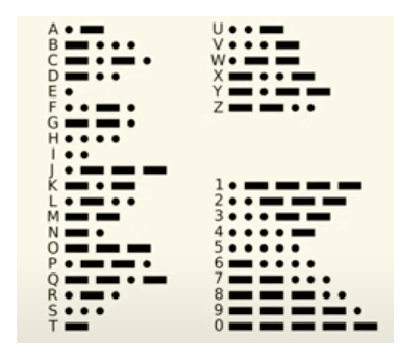
\includegraphics[width=0.3\textwidth]{lesson1/morse.eps}
    \label{fig: 1}
    \caption{モールス信号}
\end{figure}
\begin{figure}[H]
    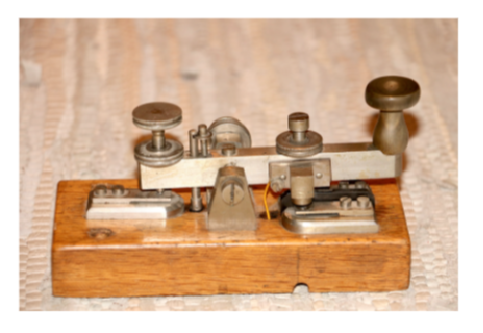
\includegraphics[width=0.3\textwidth]{lesson1/morsekey.eps}
    \label{fig: 1}
    \caption{モールスキー}
\end{figure}
\iffalse
\begin{figure}
    \centering
    \begin{minipage}{0.45\textwidth}
        \centering
        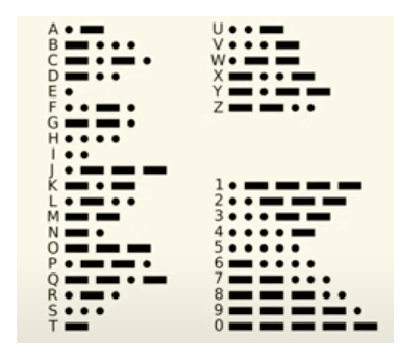
\includegraphics[width=0.9\textwidth]{lesson1/morse.eps} % first figure itself
        \caption{first figure}
    \end{minipage}\hfill
    \begin{minipage}{0.45\textwidth}
        \centering
        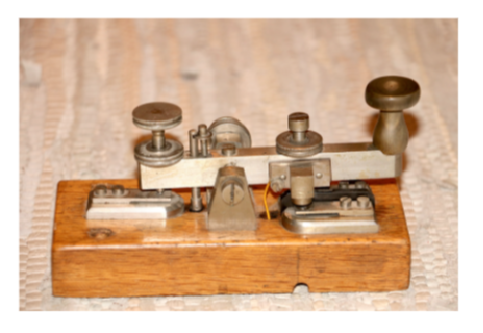
\includegraphics[width=0.9\textwidth]{lesson1/morsekey.eps} % second figure itself
        \caption{second figure}
    \end{minipage}
\end{figure}
\fi


モールス信号が電子信号を使うことにして、
こういう機械を使ってたんですね。パタパタと打ち込むと、それが
電子の回路が繋がったり離れたり外したりするとこれが信号のオンとオフをになることなんですが、そうすると短点と長点(短いものと長いもの)で2つの信号の種類があるんですが、英語では、「ダッシュ、ドット、ダッシュ、ドット」と読み方をするんですが、日本語では「ツー、ドン」だと思います。
「ツー、ドン、ツー、ツー、ドンドン」
すると、メッセージが伝えるようになります。そういうふうに読み、アルファベット順にできます。長いメッセージと短いメッセージがあって、一番良く使われているものは
アルファベットのレターとして「E」なので、それ一番短いメッセージです。あまり使われてないアルファベットの記号はそれ長いメッセージになっているんですが、それが「X」 とか「G」 とか、そういうふうなんです。この技術を利用し、数分でアメリカの東海岸から西海岸までメッセージを通信できるようになりました。さっきのシステムと同様に、中継所を使わなければならなかったんですが、一つの信号は数千キロぐらいまで通信できるようになってなかったので、途中で誰かが聞いて、書き出し、同じメッセージをもう1回次の中継所まで送る制度になってました。この新技術はさっき話したポニーエクスプレスやナポレオンの腕木通信機が使われなくなった原因です。もちろん、モールス信号にも短所があります:
\begin{enumerate}
    \item 「難易度高い」:違う通信手法と比べると、訓練も必要なんです。訓練されていない人ははあまりメッセージがを読んだりとか聞いたりとかできないものなんですよね。
\end{enumerate}

そうすると、続きの技術としてには 電話になっていたんですが、その電話が
\textbf{初めて長い距離でボイス}の通信ができるようになりました。自分の声で通信でできるようになりました。これは一番最初の方は、ポイントツーポイントなんですが、 Aさんの家からBさんの家にメッセージを伝えるようにしたいなら、その間には直接電線を引っ張らなきゃいけなかったです。もちろんこの方法には限界があるんです。
% Insert point-to-point pic here
\begin{figure}[H]
    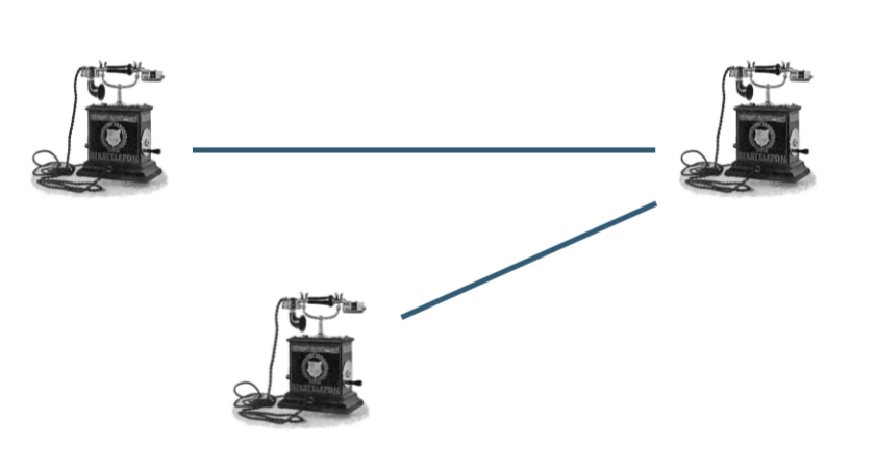
\includegraphics[width=0.8\textwidth]{lesson1/pointpoint.eps}
    \label{fig: 1}
    \caption{ポイントツーポイント手法}
\end{figure}


その後の進化としては、ネットワークの真ん中にはスイッチボードという概念のを作って、それを入れたんですが、そうすると自分の家かからそのスイッチボードのところに繋がって、最初にはスイッチボードのところに誰かが電話が出て、「じゃあ、Aさんお願いします」と言って、そのスイッチボードのオペレータが自分の家とAさんの家と繋げることで直接つながることになったんです。
% Insert switchboard pic here.
\begin{figure}[H]
    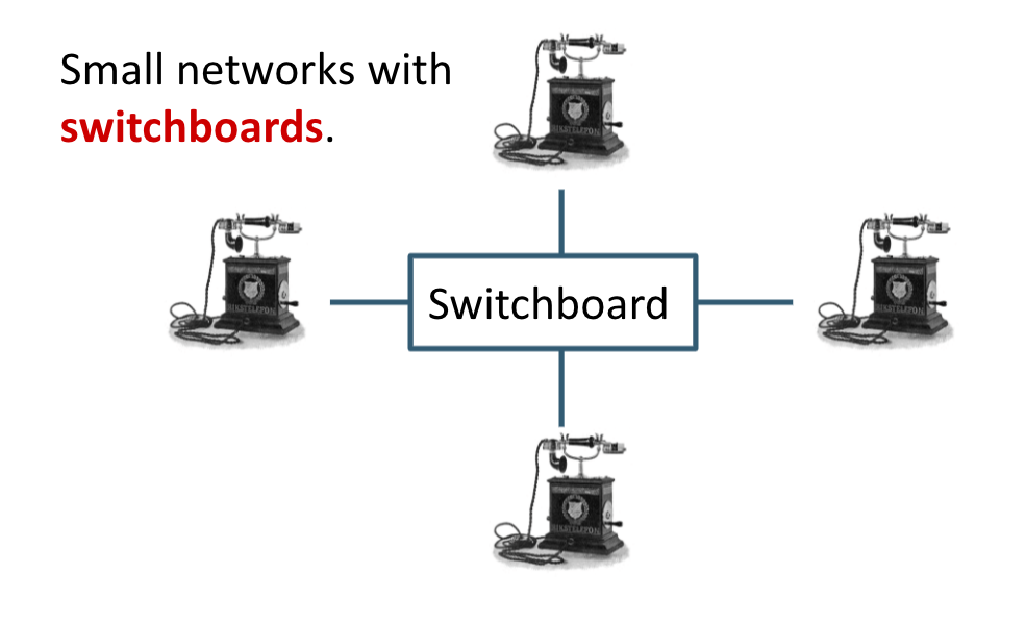
\includegraphics[width=0.8\textwidth]{lesson1/switchboard.eps}
    \label{fig: 1}
    \caption{スイッチボード手法}
\end{figure}
そうするとだんだん広がって、あっという間に世界的規模ぐらいになったんですよね。
その後は、人間のスイッチボードオペレーターが機械に変更しました。
\subsection{インターネット}
次のステップが今の使っているインターネット。インターネットというものが、全世界規模と地球規模の「ネットワーク of ネットワークス」なんですよね。
% insert internet pic here
\begin{figure}[H]
    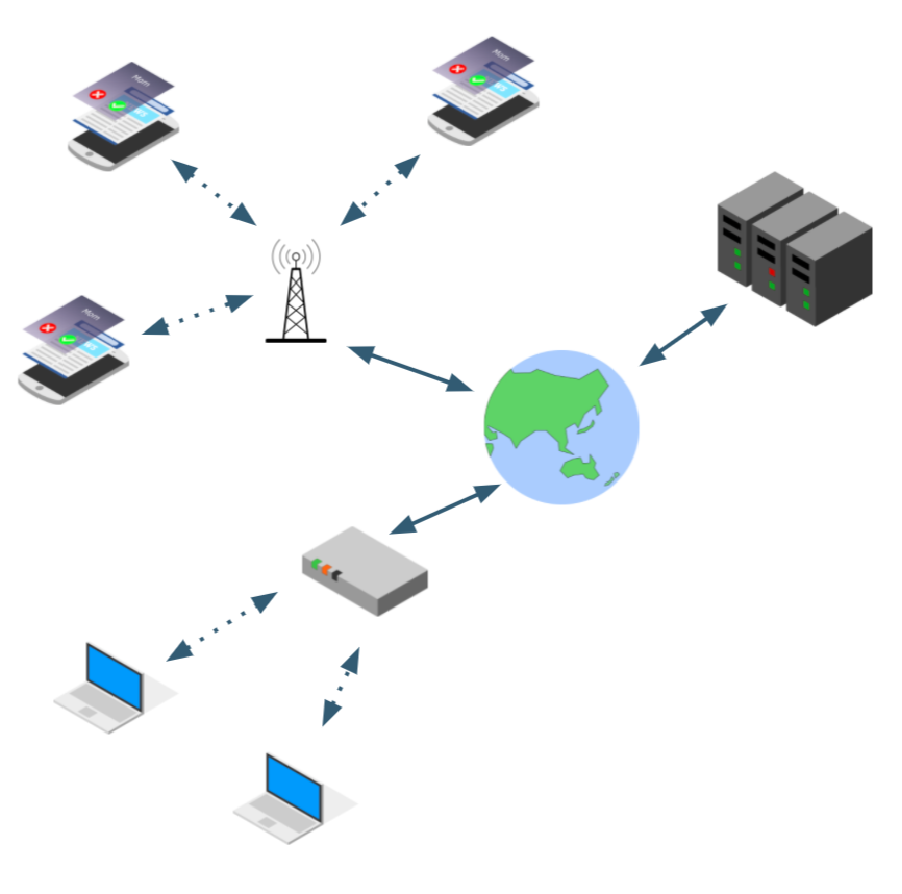
\includegraphics[width=0.8\textwidth]{lesson1/internet.eps}
    \label{fig: 1}
    \caption{インターネット}
\end{figure}
各ところにはネットワークがあって、そのネットワークとネットワークの間の通信があって、それがインターネットワークと呼んで、それを短く呼ぶと「インターネット」になって全世界の一つの通信できるようになりました。
これが例えば、携帯電話のタワーから、自分の持っている携帯からタワーまで通信して、その後はインターネットルーターという機械まで繋がって、その後は向こう側にあるサーバーコンピューターに繋がって、Googleに繋がったりとか、Amazonにつながったりとか
いろんなサービスに繋がることができます。
音声ビデオ、エンターテインメントのいくつかの種類なんですけど、もちろんそれがインフォメーションサービス、これが銀行とか電子メールとか、人と人と、サービスまでの繋がりとかそれが「P2P」、「BtoB」いくつかの略語があって、それがいろんなコミュニケーションのパターンになっているでしょう。このインターネットが良いのは、世界の一番重要な通信基盤になっているんですよね。いくつかのアプリケーションができるようになりました。
% insert picture here
\begin{figure}[H]
    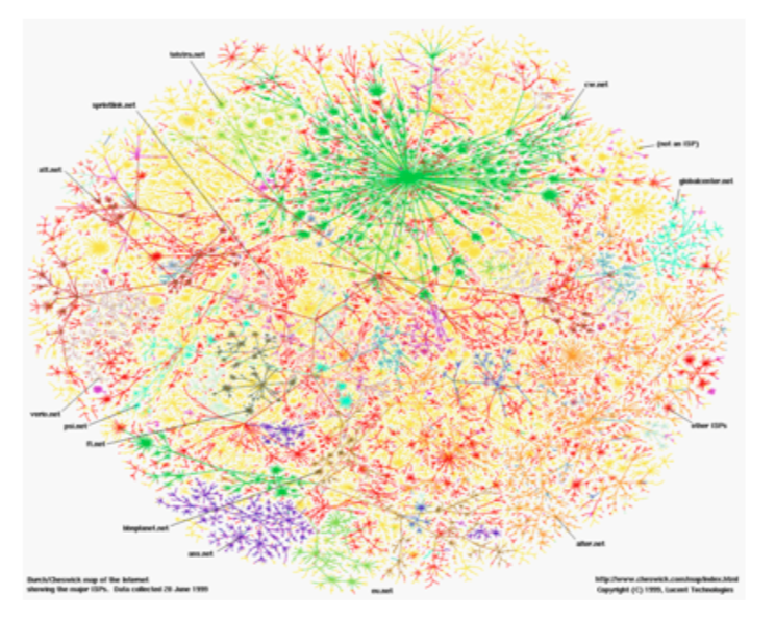
\includegraphics[width=0.8\textwidth]{lesson1/internetmap.eps}
    \label{fig: 1}
    \caption{ネットワーク of ネットワークス}
\end{figure}
先の言ってた通りでインターネットというのは、「ネットワーク of ネットワークス」なんですが、\textbf{Figure 1.10}が1999年の地図なんですが、この地図では線と点のところ、丸のところがあるんですけれど、それが線が物理的な回路じゃなくて、丸がコンピュータとかノードじゃなくて、丸がネットワーク。線がネットワークとネットワークの間の通信する契約がある状態なんですけども、そうするとこの地図が8万個ぐらいのネットワークに繋がっていると思います。これが、今からこれがこのモジュールのやる、量子通信の基礎のことが、この視点から始まります。

\section{アナログからデジタルへ}

\subsection{紹介}
通信したい場合にはどういうふうに抽象化できるのでしょう。
\begin{figure}[H]
    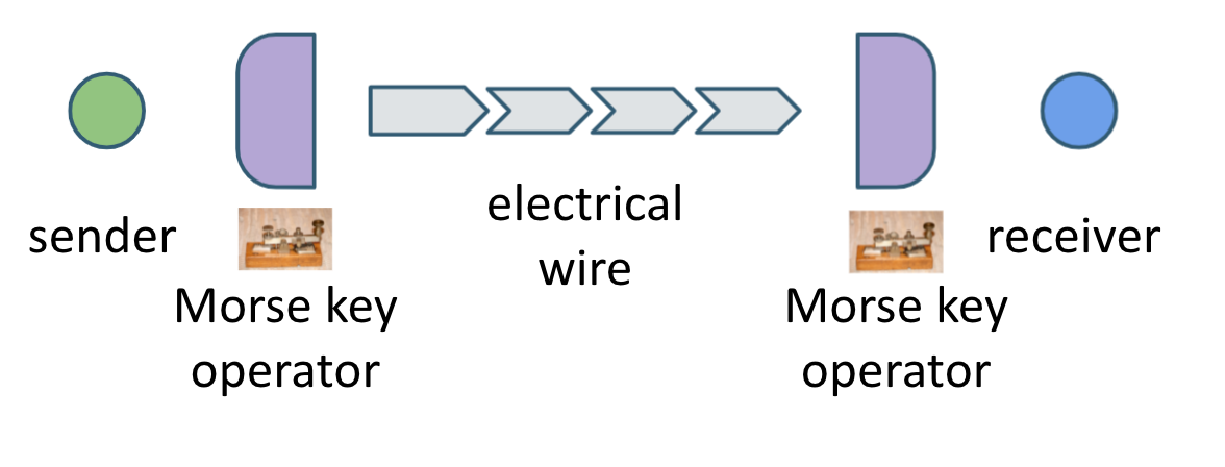
\includegraphics[width=0.8\textwidth]{lesson1/sender_receiver.eps}
    \label{fig: 1}
    \caption{受信者・送信者}
\end{figure}
センダー(送信者)とレシーバー(受信者)といるんですが、そのメッセージを何かでエンコードしなければならない。そうすると、メッセージを伝えて、向こう側にいる相手のいるところにはデコーダーをつけて、メッセージを受信者が読めるようになります。例えば、さっき話をしていたテレグラフ(電信機)としてはモールス信号を使って、それが電子の信号になって、電子の信号が向こう側に届いて向こうにいるモールスキーオペレーターの人が、その電子信号が聞こえて、その後はそれをアルファベットの記号に戻して、メッセージを受信する受信者がそのメッセージを読めるようになります。

さて、こういうふうに考えると、最善の通信手法は何んでしょう?
\subsection{アナログとは?}

我々はアナログの人間なんですが、世界もアナログなんですよね。
「アナログ」と言えば聞く音楽とか、自分の声とかです。あとはタッチ(触る事)です。温度がわかったりとか、材質がきめ細かいだとか、粗いだとかわかったりすることができるのです。あとは、「目」で見えるところ。色もアナログの信号なんですが、それが強いか弱い光か、どんな周波数があるのか、どんな波長があるのか。すると、色も変わるでしょう。
そういう意味で、私たちの世界にはアナログのデータが多いのです。人間はそのアナログのデータの処理は得意なんですね。


さあ、一番最初に考えられる手法としては、メッセージもアナログの手法で通信した方がいいんじゃないですか、とが自然的に思うでしょう。そうすると、これが連続的な信号なのですが、音楽とかあるんですが、そういうアナログ信号が時間が経つと信号の価値が変わるんです。エンコードすると、いくつかのところを使って受信側では、その信号を頂いて、それをデコードすると、そのメッセージが取り戻せるでしょう。

% insert continuous signal picture.
\begin{figure}[H]
    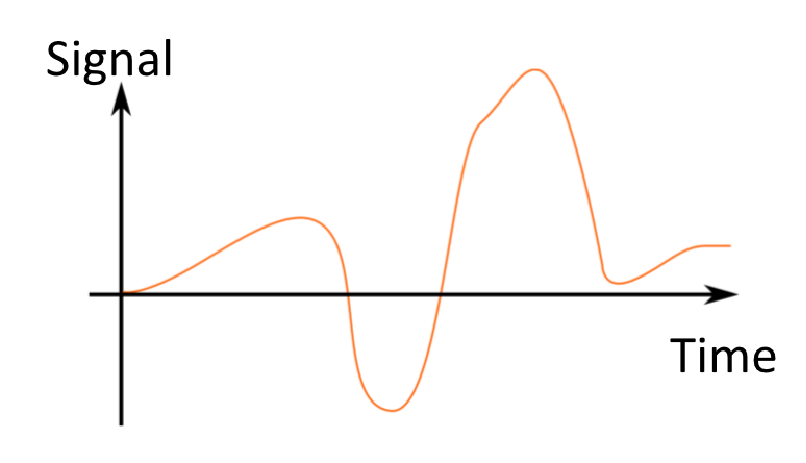
\includegraphics[width=0.8\textwidth]{lesson1/continuoussignal.eps}
    \label{fig: 1}
    \caption{アナログ通信}
\end{figure}

例えば、\textbf{Figure 1.12}のような上がったり下がったりする信号は電話とAMラジオとかでみえる信号の手法です。この場合は、いくつかの問題があるのです:
\begin{enumerate}
    \item 「ノイズ」: ノイズに弱いんです。小さい差があると、それは誤差になる。大きな変化になる場合もありますしそれをコピーすることも難しいんですね
\end{enumerate}

さっきセクション1.1で話してた腕木通信やテレグラフは中継所でメッセージをコピーしてたんですが、それがアルファベットを使ってたから、エラーになる場合は
このアナログの信号より少と思えます。
% insert continuous signal w/ disruptive noise included here. 
\begin{figure}[H]
    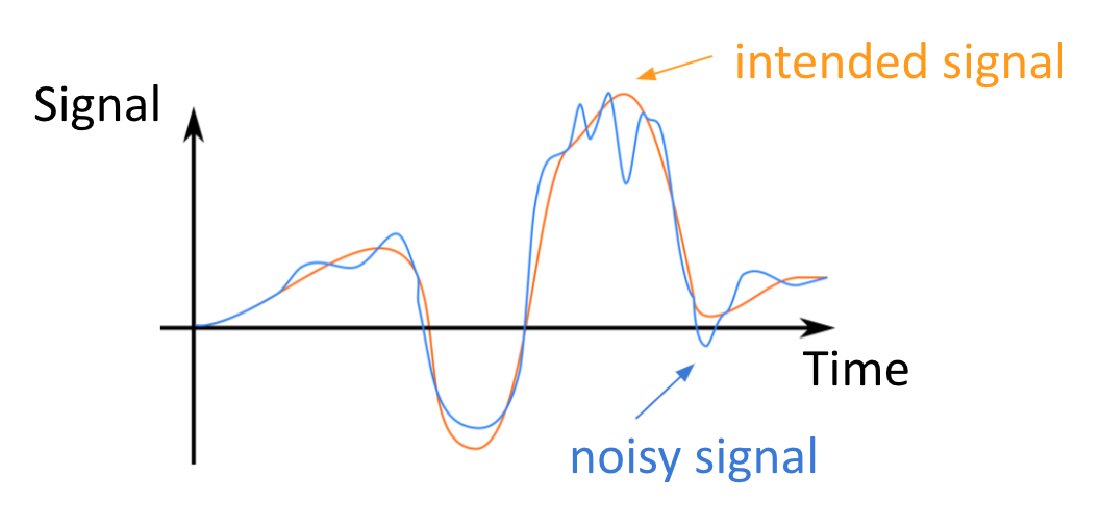
\includegraphics[width=0.8\textwidth]{lesson1/continuous_signal_noise.eps}
    \label{fig: 1}
    \caption{アナログ通信 + ノイズ}
\end{figure}

\textbf{figure 1.13}は\textbf{figure 1.12}のオレンジの信号があったところに、ノイズが入ってきてコピーした場合にこの青い線になる可能性があることを示しています。それは音楽だったら、どのぐらいのノイズが影響するのか。まぁ、機械と信号と人次第なんですが、大きな問題になる場合もありますね。
\subsection{デジタル}
さて、アナログじゃなくてデジタルの信号が使えることは可能なんですが。例としては、腕木通信機とかテレグラフとかを使うと、離散する設定を使うんです。連続信号をデジタルにする場合には、どうすればいいでしょう。
% Insert discrete digital signal pic  w/ t_0, t_1, t_2 here
\begin{figure}[H]
    \centering
    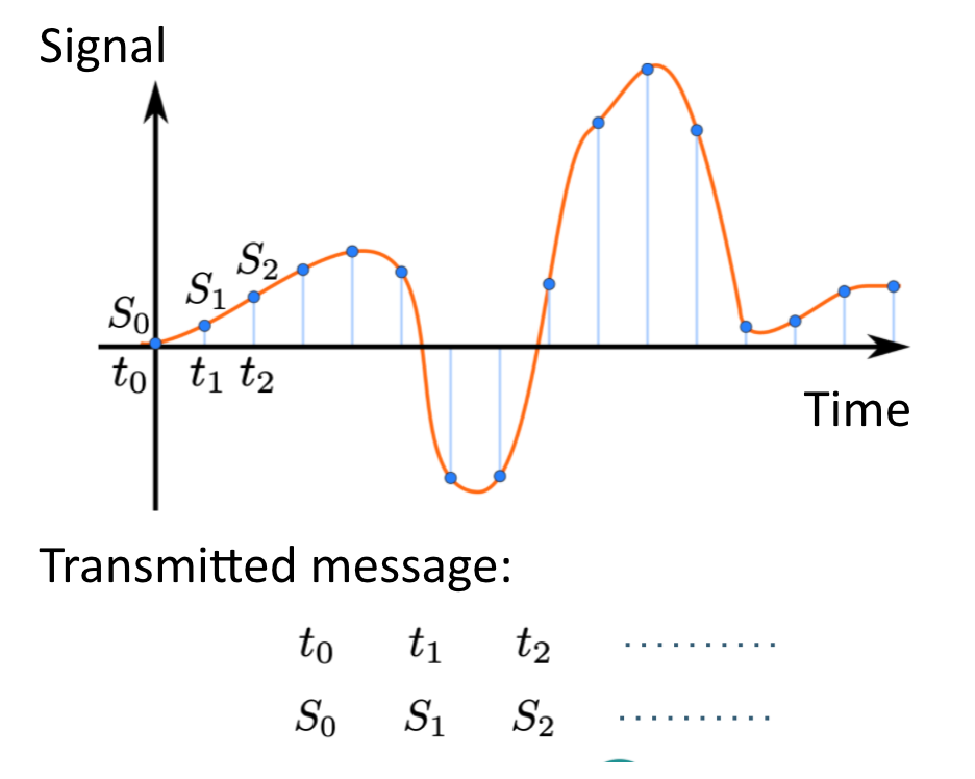
\includegraphics[width=0.8\textwidth]{lesson1/discre_signal.eps}
    \label{fig: 1}
    \begin{center}
        \caption{離散通信}
    \end{center}
\end{figure}
そうすると、\textbf{figure 1.14}で見えるように時間の軸としては信号があるのですが左から右に行くと時間が経つんですよね。すると、その青い所で定時的にその信号を測定しています。その測定されていることが、この青い棒の高さを記録すると信号になるんですね。そうすると、$t_0$、$t_1$、$t_2$には連続でタイムスロットで信号のことに
なるんですが、その場合だったら例えば、$t_0$のところには「$s_0$」になる、$t_1$のところには$s_1$になる、$t_2$のところには$s_2$になるように連続でやります。これの精度が、どのぐらいの頻度でサンプリングすることに依存するんです。低い頻度だと精度が低くなるので、)信号が早く変わってしまう期間には、頻度高くサンプリングすることが必要なんです。
fig[Z]の場合だったら、左側はゆっくり信号が上がってきてるんですが、中部では急に変更しますので、サンプリング率を高める必要があります。中部でサンプリングしなかったら、信号が下がっている箇所の記録にミスする可能性があって、信号の誤差になるんですね。
デジタルの長所:
\begin{enumerate}
    \item 「アンチノイズ」:デジタルの信号はアナログの信号の比較するとより強いんです。さっきのアルファベットの例を考えると、アルファベットは離散的なメッセージになるんです。
    \item  「予算的」:コストは安い。システムの処理も意外と簡単。使う手法によるんですけれども、帯域を使う効率が高いのです。
\end{enumerate}

\section{情報単位としてのビット}
\subsection{デジタル信号の表し方}
さて、こういうデジタルの信号はどうやって表示できるようにはなるでしょう。
先の例に戻って、ナポレオンの腕木通信機なんですが、これがいくつかの形があるんですよね。
% insert war is over
\begin{figure}[H]
    \centering
    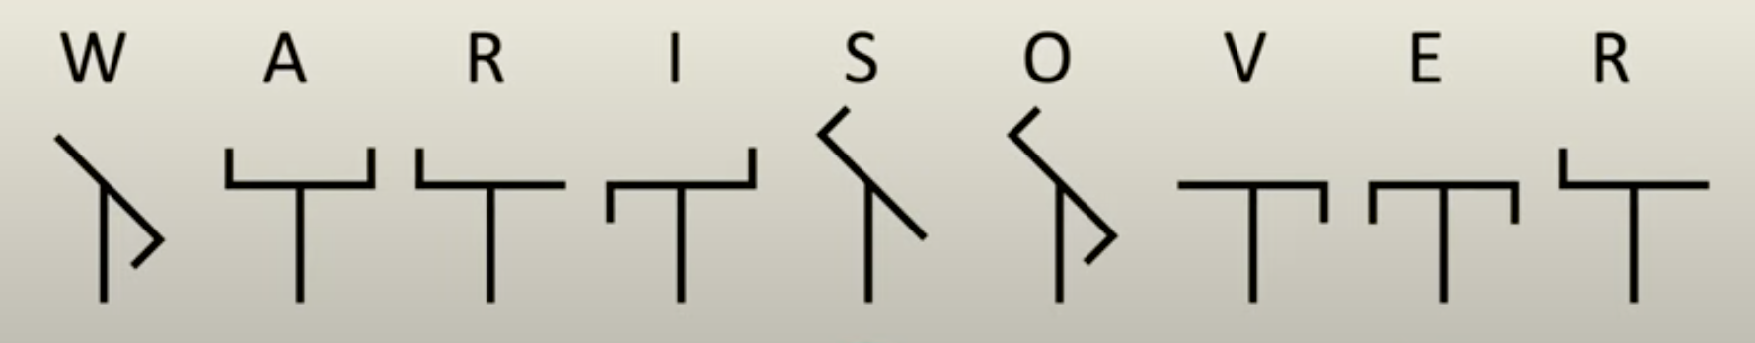
\includegraphics[width=0.5\textwidth]{lesson1/warisover.pdf}
    \label{fig: 1}
    \begin{center}
        \caption{例:腕木通信機}
    \end{center}
    
\end{figure}

例えば、このメッセージを伝えたい場合には、「War is over. (戦争が終わった)」こういうふうに示すんでしょう。こういう形にすることなんですが、どれぐらい大変なのでしょうかね。これは物理的に変更しなければならないんですが、配置によって変換することは
簡単かもしれないんですが結構人力が必要な場合もあります。
% Insert A -> R, W -> 10 
\begin{figure}[H]
    \centering
    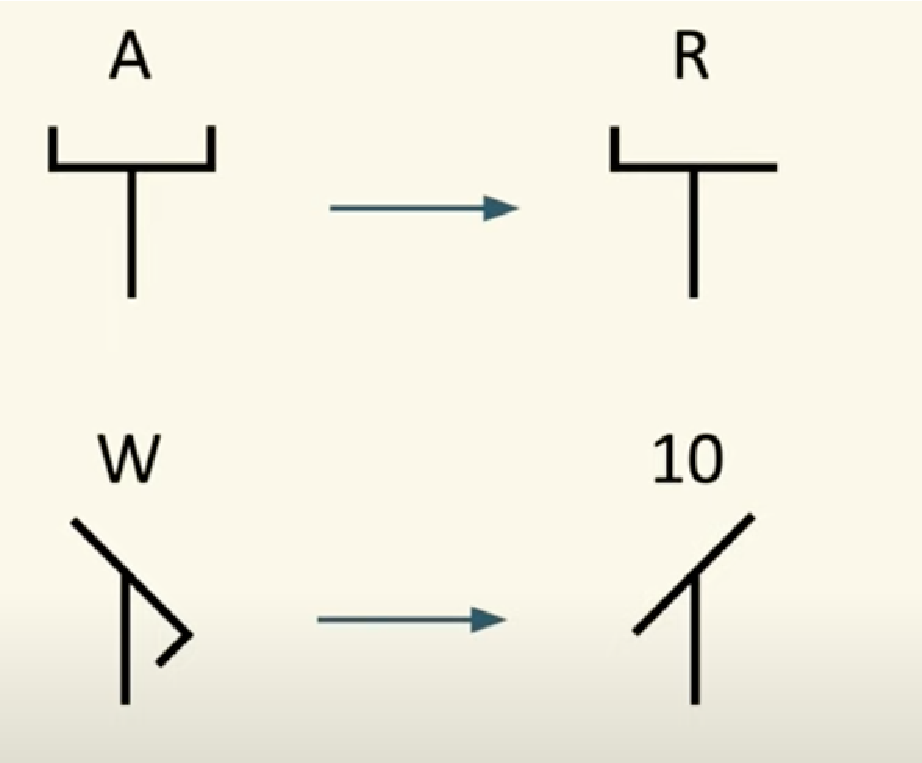
\includegraphics[width=0.8\textwidth]{lesson1/a_to_r.pdf}
    \label{fig: 1}
    \begin{center}
        \caption{例2:腕木通信機}
    \end{center}
\end{figure}
\textbf{Figure 1.16}ご示すのように、「A」から「R」なんですが、
は簡単な変換ですが「W」から「10」までの変換は結構難しい。この処理には、メッセージを伝えるためにはどのぐらいエネルギーを使うのか。どのくらい変換することが難しいのか。もちろん時間もかかるんです。
ナポレオンの手法は、記号が26個のアルファベットと10個の数字なんですが、
そのアルファベットと記号の組み合わせの数全部あわせると30億くらいあるんですけれども、そうすると、それが区別できるようにしなければならないので、それが結構複雑になるんですよね。
さて、モールス信号に戻ると、記号の数はどれぐらいになるでしょう。基本的に、 2つの記号しか使わないんですが、「ツー」と「トン」ですよね。英語では
ダッシュとドット。
% Insert U encoding
\begin{figure}[H]
    \centering
    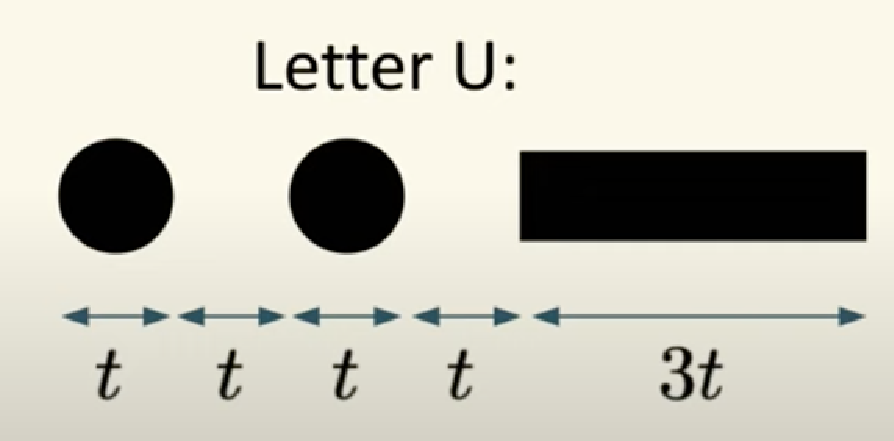
\includegraphics[width=0.8\textwidth]{lesson1/letter_u.pdf}
    \label{fig: 1}
    \begin{center}
        \caption{例:モールス信号}
    \end{center}
\end{figure}
\textbf{Figure 1.17}は\emph{U}のエンコーディングしたもので、「U」の記号としてはこれになるんです。
そうすると、短い時間はtを使って長い時間は3tを使うことにするんです。そうすると、早く変換できるようになるでしょう。
さて、こういう信号を伝えたい場合には、物理的にはどうしますかね?
\subsection{ビット (bit)}
% insert morse graph
\begin{figure}[H]
    \centering
    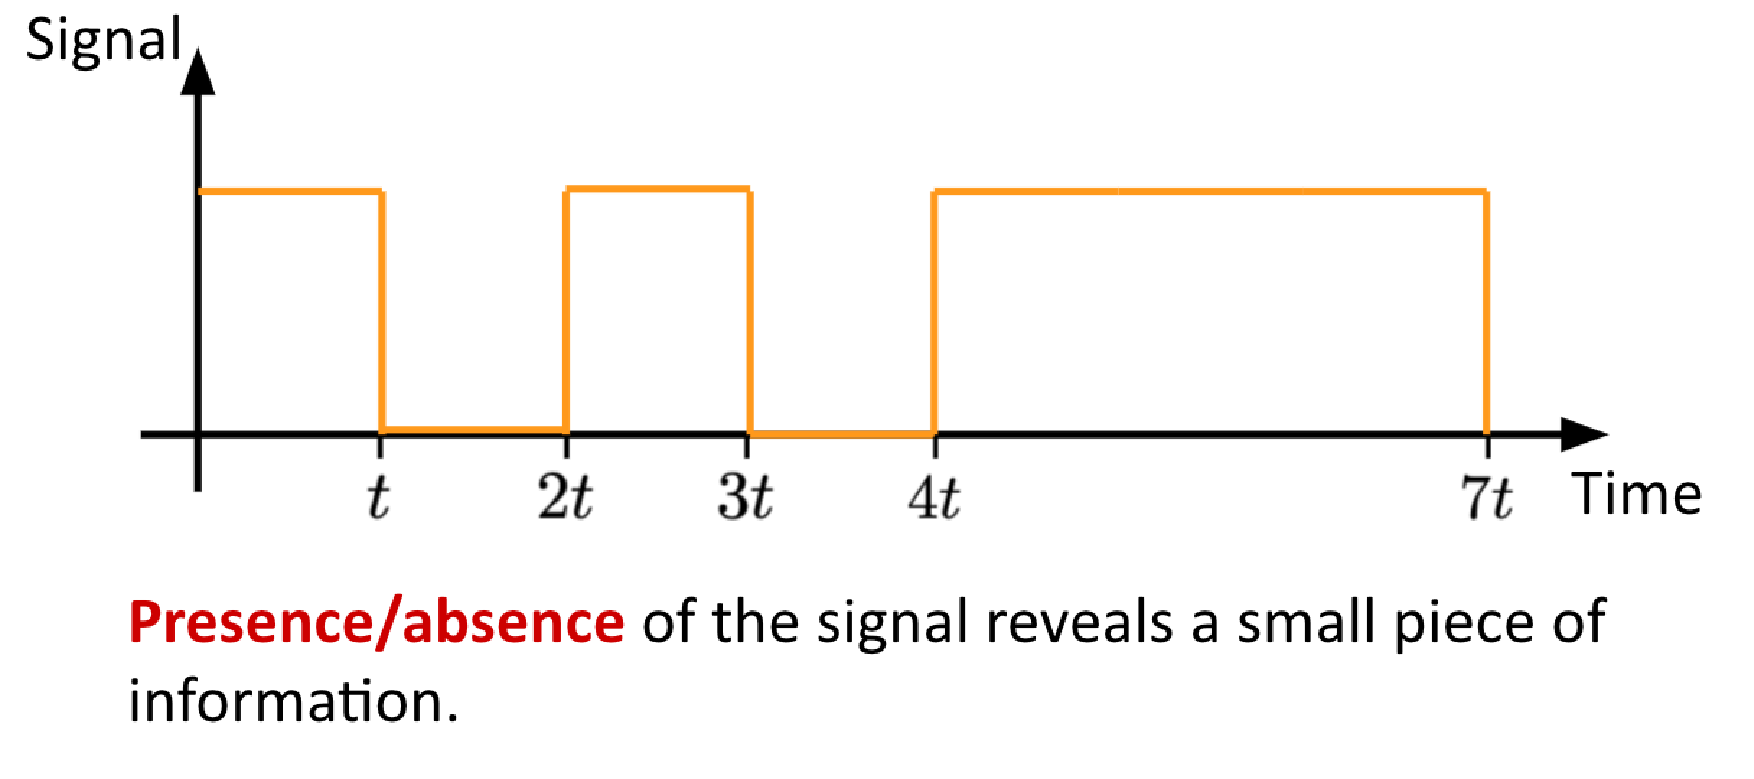
\includegraphics[width=0.8\textwidth]{lesson1/presence_abscence.pdf}
    \label{fig: 1}
    \begin{center}
        \caption{モールス信号のグラフ}
    \end{center}
\end{figure}
信号が\textbf{Figure 1.18}のふうにする場合があるんですが、例えばこれが左から右にいくと、これが時間軸なのですが、この信号は物理的には、例えば電圧なんです。
高い電圧が「1」、低い電圧が「0」の場合とすると0と1じゃなくて、この場合だったら「ドン」+「短いスペース」+「ドン」+「短いスペース」+「ツー」になるんですよね。この信号があるとない場合だけには、情報が伝われます。

一番ちっちゃい情報の単位は「ビット (bit)」になります。バイナリーデジット (binary digit)の略なので、これが「bit」となる。これが、コンピュテーションとコミュニケーション、計算と通信両方によく使う単位です。多分ご存知だと思います。これが「true/false(真偽)」と「yes/no」と「on/off」
のようないくつかのブーリアン(論理型)の型があるんですが、基本的にすべてを考えると、よく使う表現としては「0」と「1」なんですよね。
ビットの長所は「ノイズ(雑音)に強い所です。
\begin{figure}[H]
    \centering
    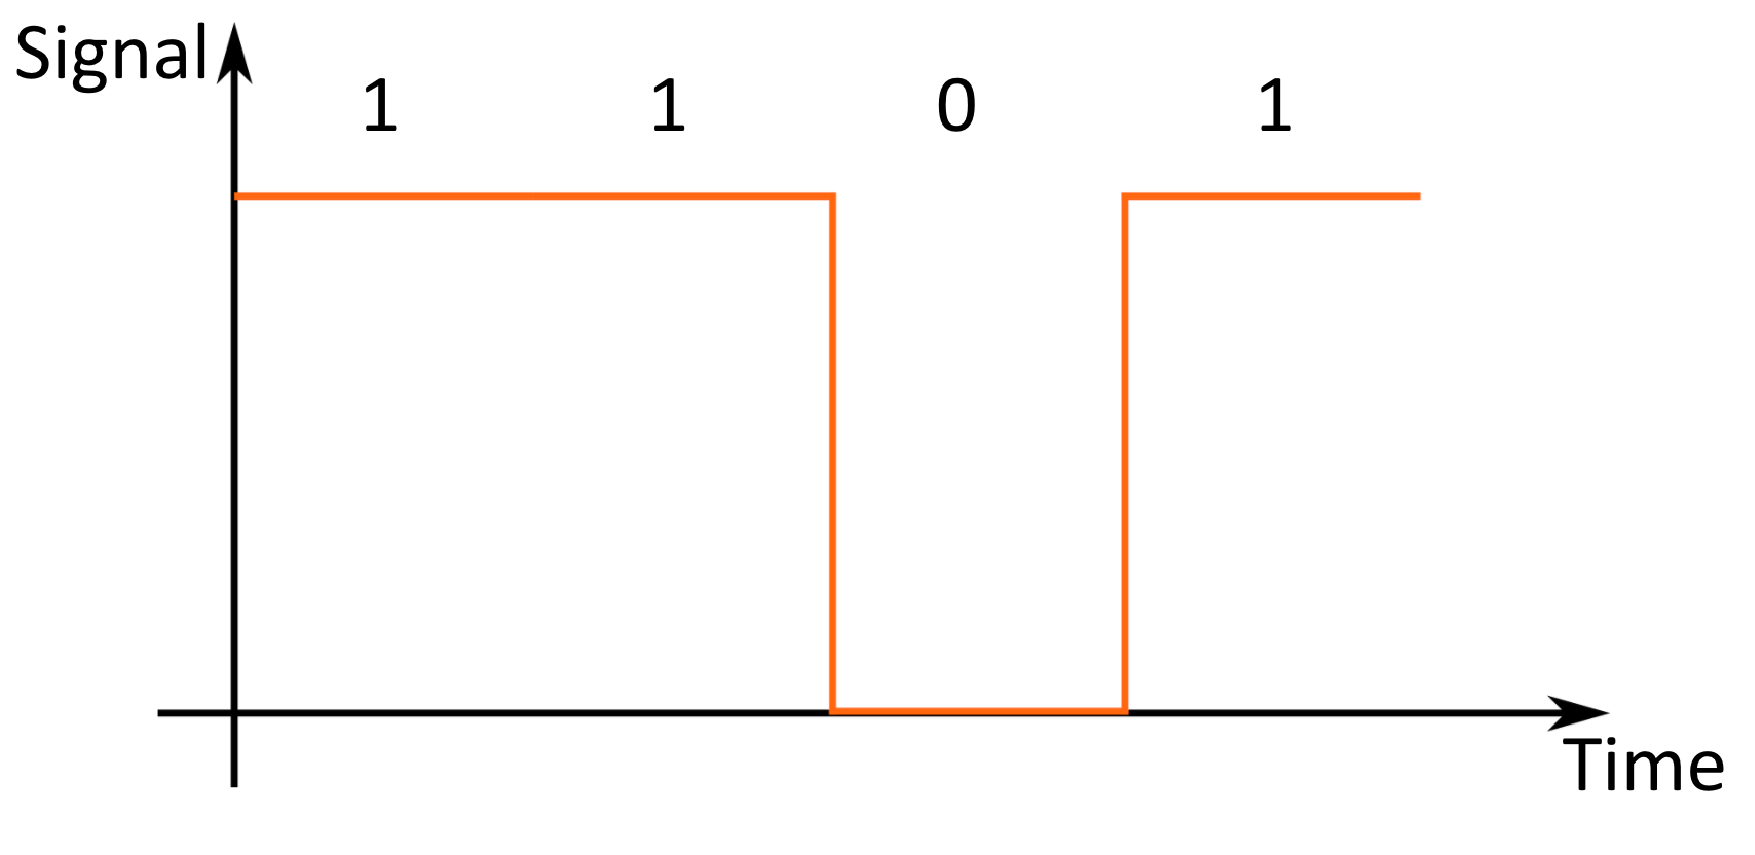
\includegraphics[width=0.8\textwidth]{lesson1/presence_abscence_bit.pdf}
    \label{fig: 1}
    \begin{center}
        \caption{ビットのグラフ}
    \end{center}
\end{figure}
この場合には、見える通りなんですが、この電圧が高いところと、電圧が低いところは結構離れてますよね?これが区別しやすいので、これが、今信号が高いところに「1」「1」で、低いところは「0」、高いところには「1」に戻る。
% insert graph w/ noise
\begin{figure}[H]
    \centering
    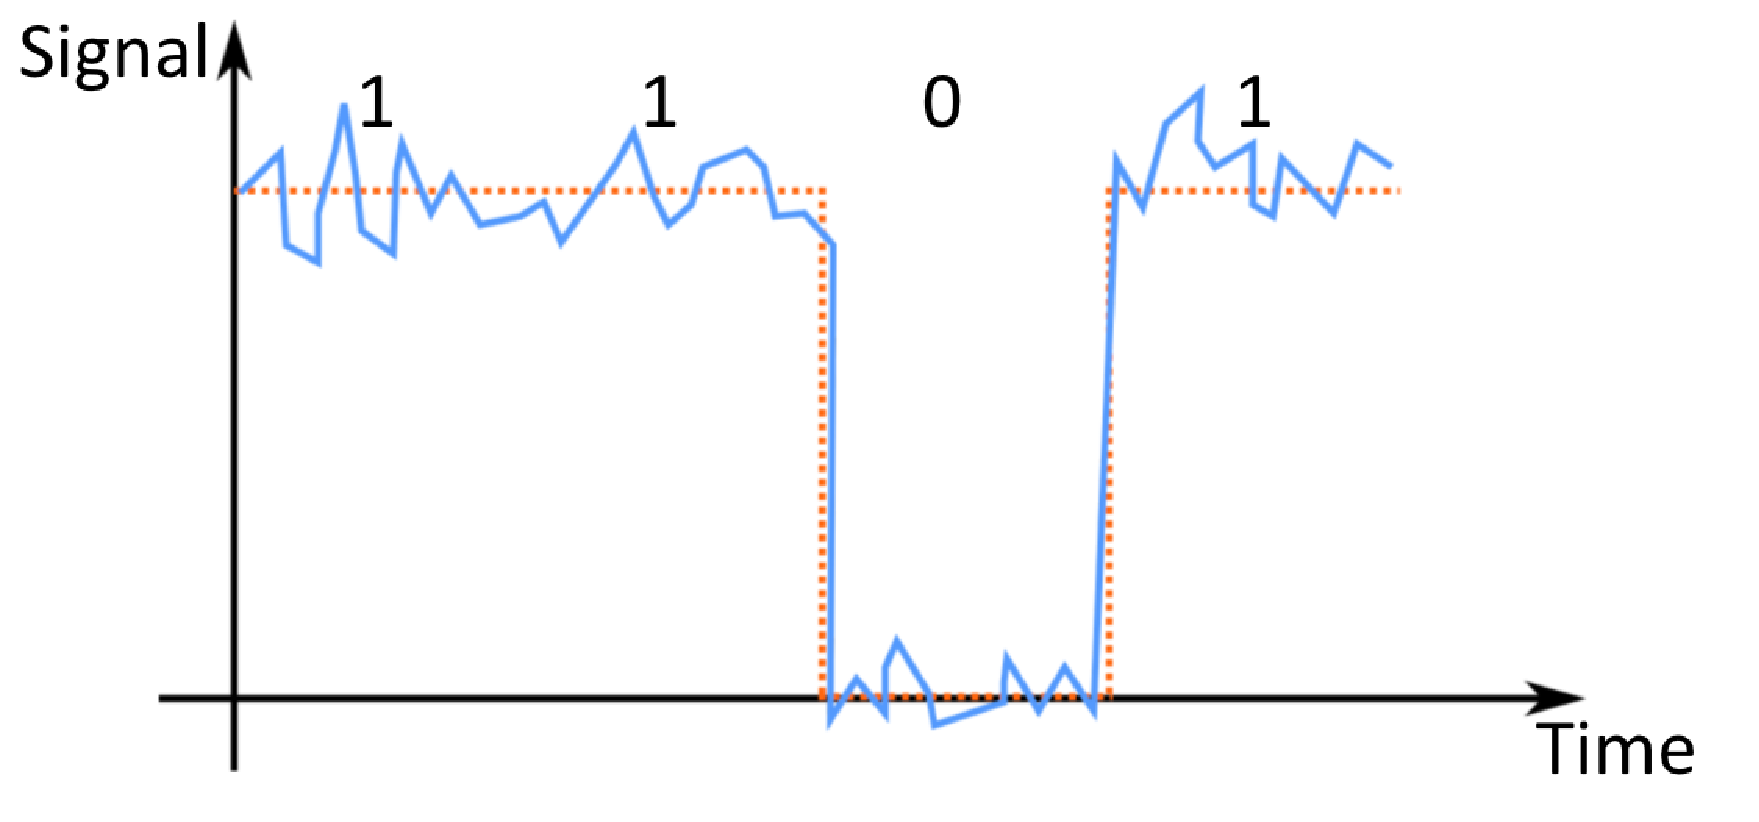
\includegraphics[width=0.8\textwidth]{lesson1/presence_abscence_noise.pdf}
    \label{fig: 1}
    \begin{center}
        \caption{ビットのグラフ}
    \end{center}
\end{figure}
ノイズがかかる場合を想定すると、\textbf{Figure 1.20}のふうになるかもしれないんです。それでも、上の段と下の段は区別はしやすいと考えられると思います。
\subsection{二進法}
さて、これがこういうふうに処理して、もともとあった信号の電圧に戻す場合はありますね。これが簡単にできるようでしょう?すると、さっきの最初の信号「1101」になってたんですがそれは取り出すことは簡単。

さて、このバイナリーノーテーション (binary notation) 。これを二進数の数え方でちょっと見てみましょう。たぶん見たことあると思いますが、念のために。
% insert bit permutations slide
\begin{figure}[H]
    \centering
    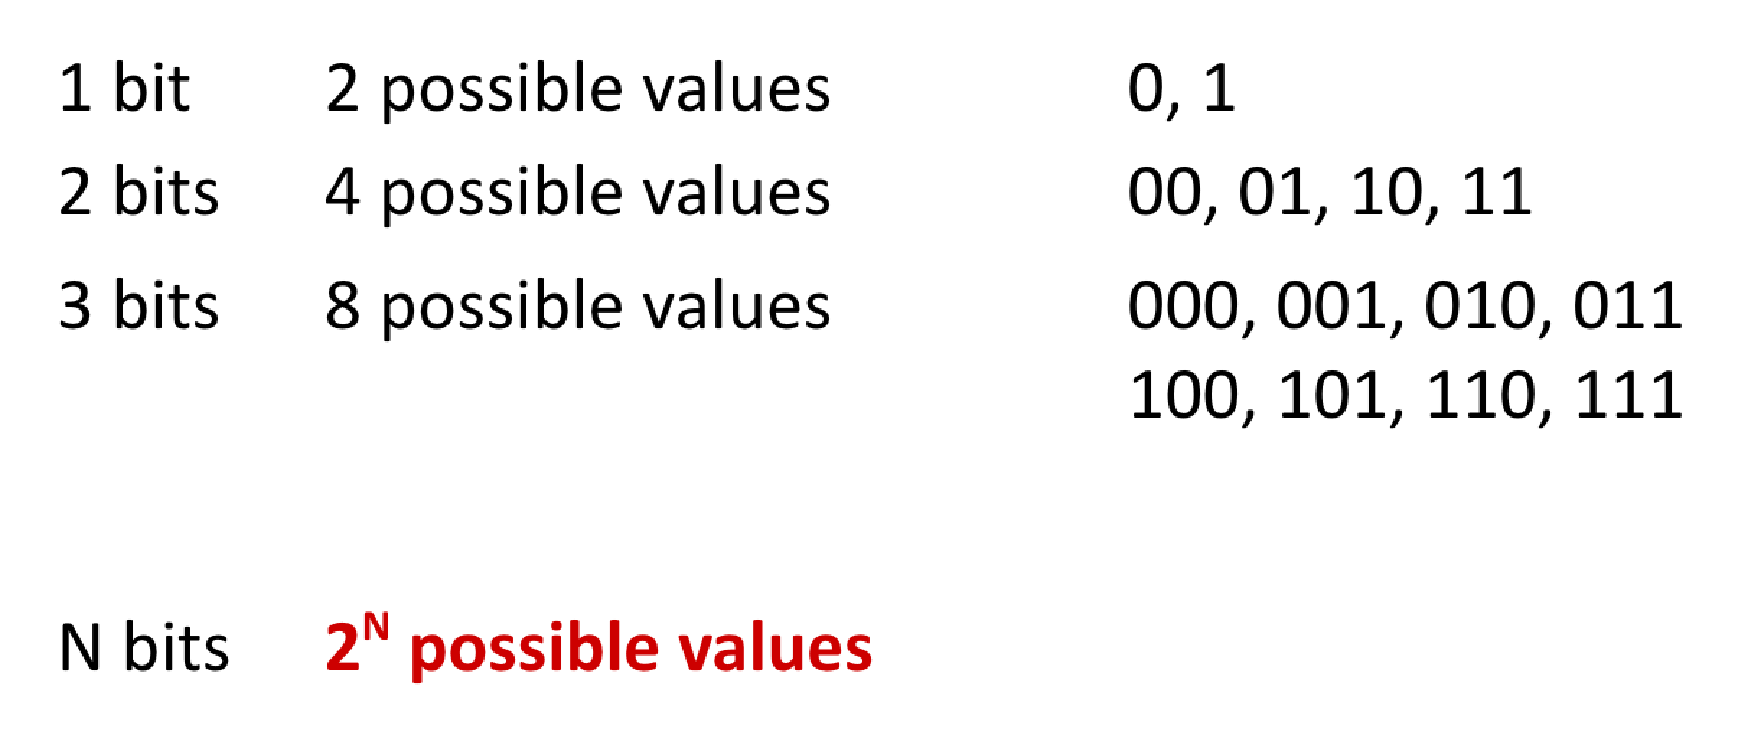
\includegraphics[width=0.8\textwidth]{lesson1/binary_notation.pdf}
    \label{fig: 1}
    \begin{center}
        \caption{ビットのグラフ}
    \end{center}
\end{figure}
一つのビットは2つの状態は可能でしょう。「0」と「1」
2つのビットだったら4つ。  「00」, 「01」, 「10」, 「11」。3つのビットだったら、8個の可能性がありますよね。000から111までで。まあ、これを繰り返すと分かると思います。けれども、
nビットを使うと2のn乗の状態は可能です。これが、2 のn乗のメッセージを伝えることは可能です。どうやって、これが十進。みなさんは小学生の頃から十進の書き方を学んでいるんですが、それがバイナリのことに変換できるんでしょう。
% insert decimal notation
\begin{figure}[H]
    \centering
    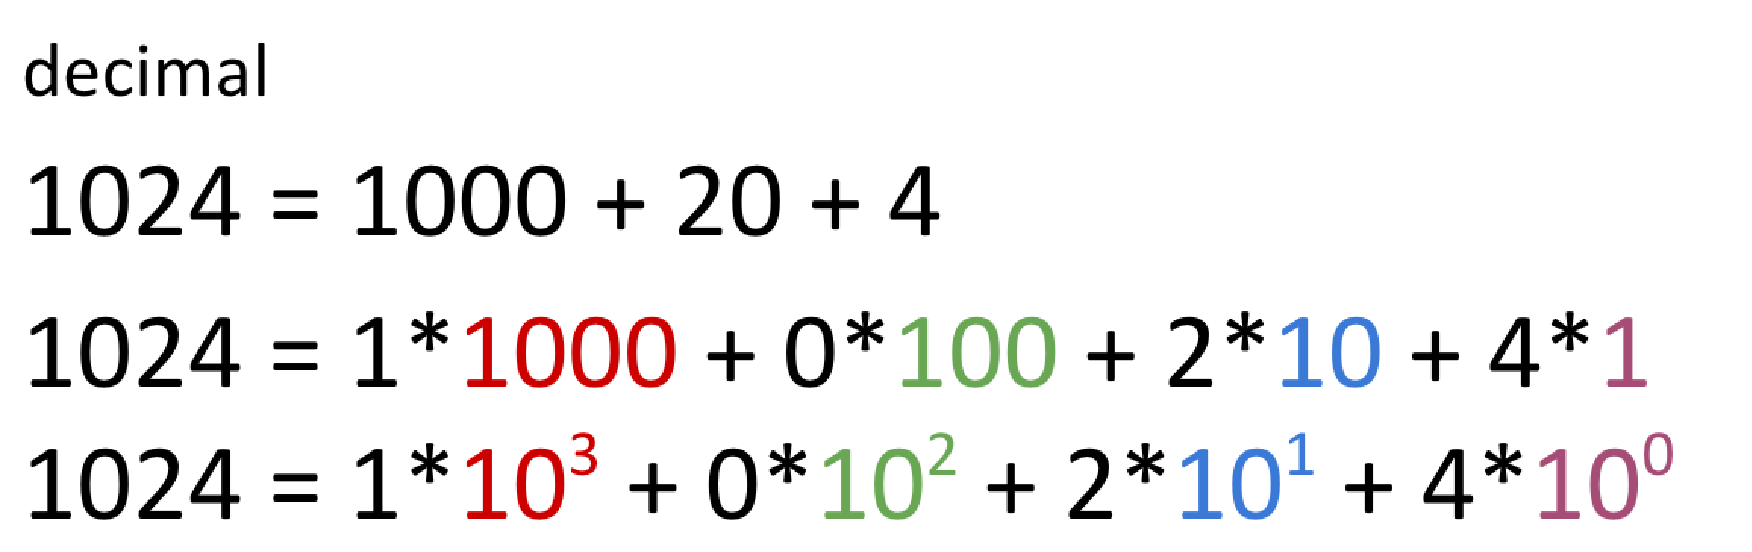
\includegraphics[width=0.8\textwidth]{lesson1/decimal_notation.pdf}
    \label{fig: 1}
    \begin{center}
        \caption{ビットのグラフ}
    \end{center}
\end{figure}
例えば、このデスマル(decimal、十進法)の場合には、
これが受信機なんですが、1024が「1000 + 20 +4」でしょう。そうすると、その最初の1が、「1 x 1000」という意味で、0が100の桁なのですが、その100の桁はないので、それは「0」を書いて続きで、2のところは、これが x 10なので、「2 x 10」最後には、「4 x 1」なんですね。もう一つの書き方にすると、「1 x 10の3乗」+「0 x 10の2乗」+ 「2 x 10の1乗」+ 「4 x 10の0乗」
これがバイナリー場合、二進でやると、これが「ベース 2 (二進数)」になるんですが、
「ベース 10 (十進数)」から「ベース 2 (二進数)」に変換することは可能です。

0:07:47.020,0:07:53.190
二進の例も見てみましょう。
% insert binary notation
\begin{figure}[H]
    \centering
    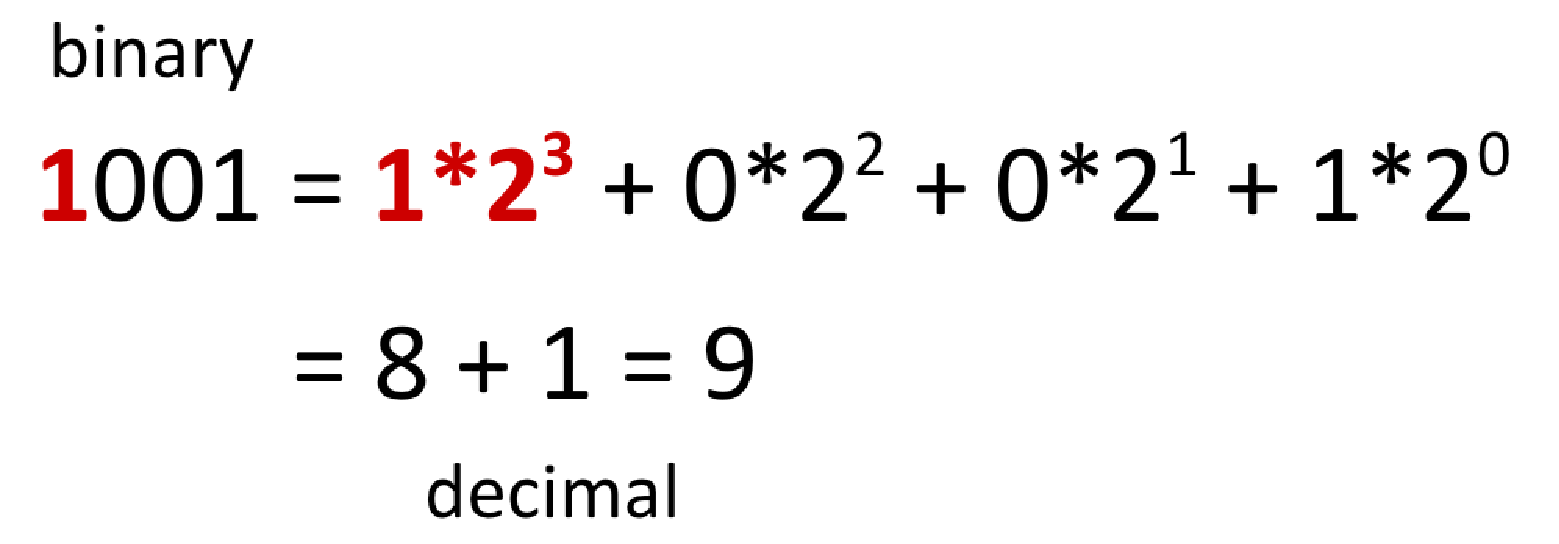
\includegraphics[width=0.8\textwidth]{lesson1/binary_ex.pdf}
    \label{fig: 1}
    \begin{center}
        \caption{ビットのグラフ}
    \end{center}
\end{figure}
これがバイナリーナンバーが「1001」だったら、それは「1 x 2の3乗」+「0 x 2の2乗」+ 「0 x 2の1乗」+ 「1 x 2の0乗」一緒なんですね。すると、その「1 x 2の3乗」が「8」なんで、一番下の桁は「1」になって、それで「8+1」は十進で 9となりますね。さて、ビットを使うことには、何が特徴で、何に役に立つのか?
\subsection{まとめ}
ビットの長所まとめ:
\begin{enumerate}
    \item 「ノイズ(雑音)に強い」
    \item 「エンコードする場合にもデコードする場合にも、結構やりやすい」
    \item 「処理することも結構簡単です」
\end{enumerate}
さて、こういう「ビット」が一番基本の概念でしょうかね?
まあ、「Yes!」なんですけれども。あとは「No!」なんですが。
「Yes!」は、古典(通信)の情報に結構使うんですが、Quantum(量子)の場合
「ビット」は一番基本の情報のUnit (単位)にはならない。そちらについては、今回のモジュールについては連続のステップでこれから説明します。



\section{量子通信}

情報が何かの物理のものに乗らなければでしょう。
それが電子でも光子でも電圧でも。さっきのナポレオンの腕木通信機では
形とか利用しているので、
それは物理的には何か利用しなければならないでしょう、情報を表示するためには。それが物理の手法で決まってるんです。
% Insert classical VS quantum slide
\begin{figure}[H]
    \centering
    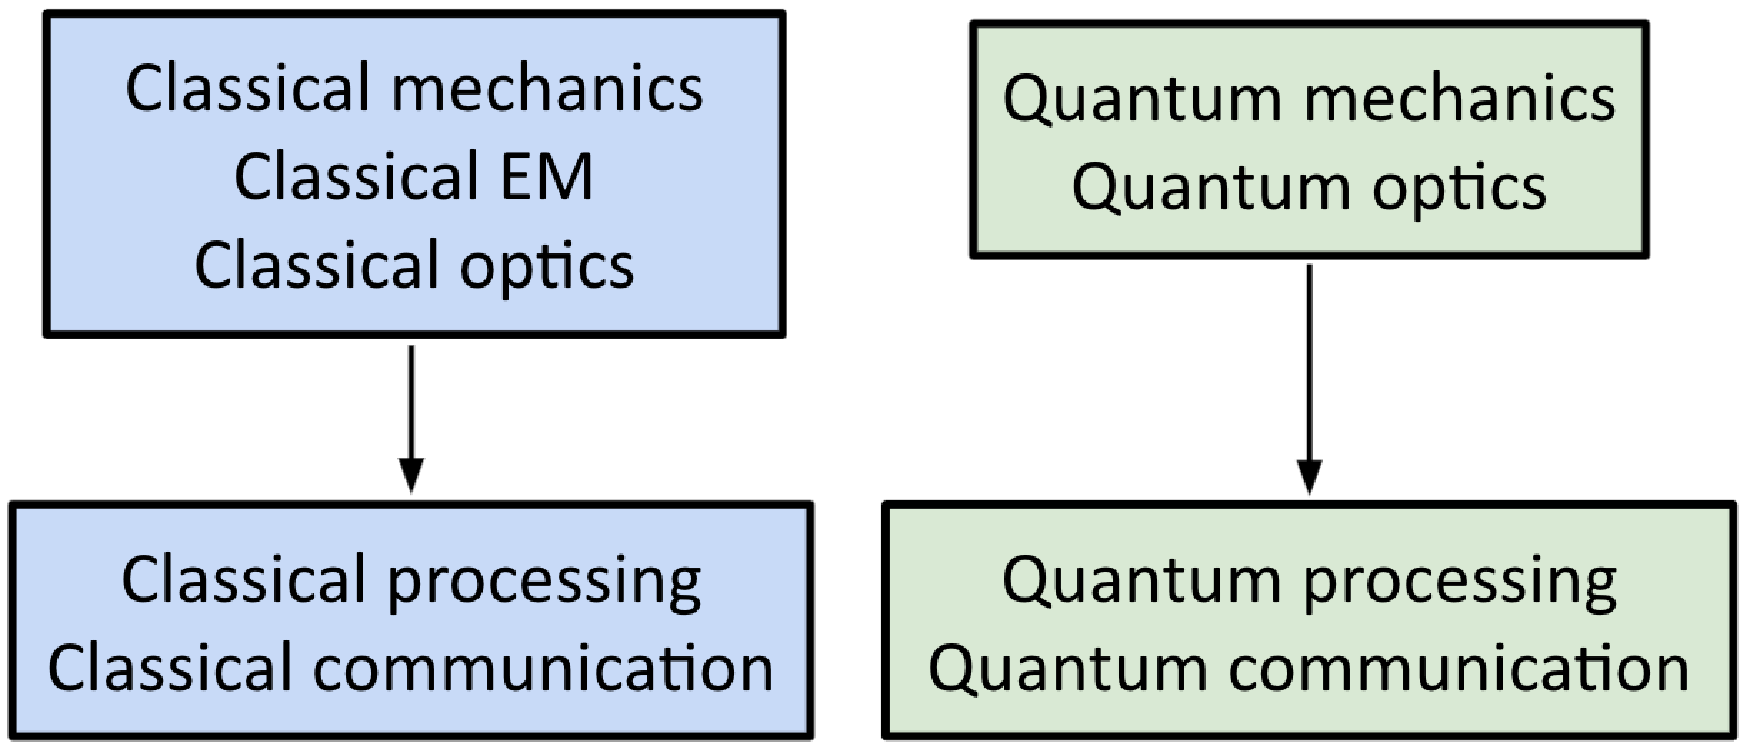
\includegraphics[width=0.8\textwidth]{lesson1/comparsion.pdf}
    \label{fig: 1}
    \begin{center}
        \caption{「古典」と「量子」}
    \end{center}
\end{figure}
決まってるんですよね、何ができるか、何が不可能か。物理的には制限されていますよね。そうすると、まぁ
古典(classical)のデータは、普通の古典力学と古典の光とか古典の光学とか、
古典のデータ処理とかによる古典通信に限られているんです。けれども、Quantum(量子)の場合だったら、量子力学 (Quantum Mechanics)と量子光学 (Quantum Optics)で決まっているんです。
そうすると、量子処理 (Quantum Processing)と量子通信(Quantum Communication)が行われます。

\subsection{古典力学の限界}
さて、量子力学が一番基礎の部分なんですよね。現在のこの宇宙でこれより精度が高い理論がないんですが。詳細なもので表現できるようになるでしょう。直感的ではないことに、結構行う場合があるんですが、まあそれがちょっと使えることが目的なんですね。これが実験ではすごく細かい精度まで調べてるんですが、それは精度はすごく高いんですよね。ですが、新しい手法と観測で見つかることになるかもしれないですが、それぞれの新しいデータの処理の手法が見つかる可能性はあると考えられると思います。実用的な理由で


なぜこれが使いたいのか、何が使えるのか?皆さんの使っている古典コンピュータと皆さんは携帯とかで見ているかもしれないし、ラップトップで見てるかもしれないんですがその中には一番基礎な、一番小さい信号を持つ措置とかとデータの処理する装置とかは、transistor(トランジスタ)と言いますね。そのトランジスタの数で、 一つの機能なんですがそれがコンピュータチップの
トランジスタの数が増えると、できる機能が増える可能性はあるんでしょう。
% Moore's law graph
\begin{figure}[H]
    \centering
    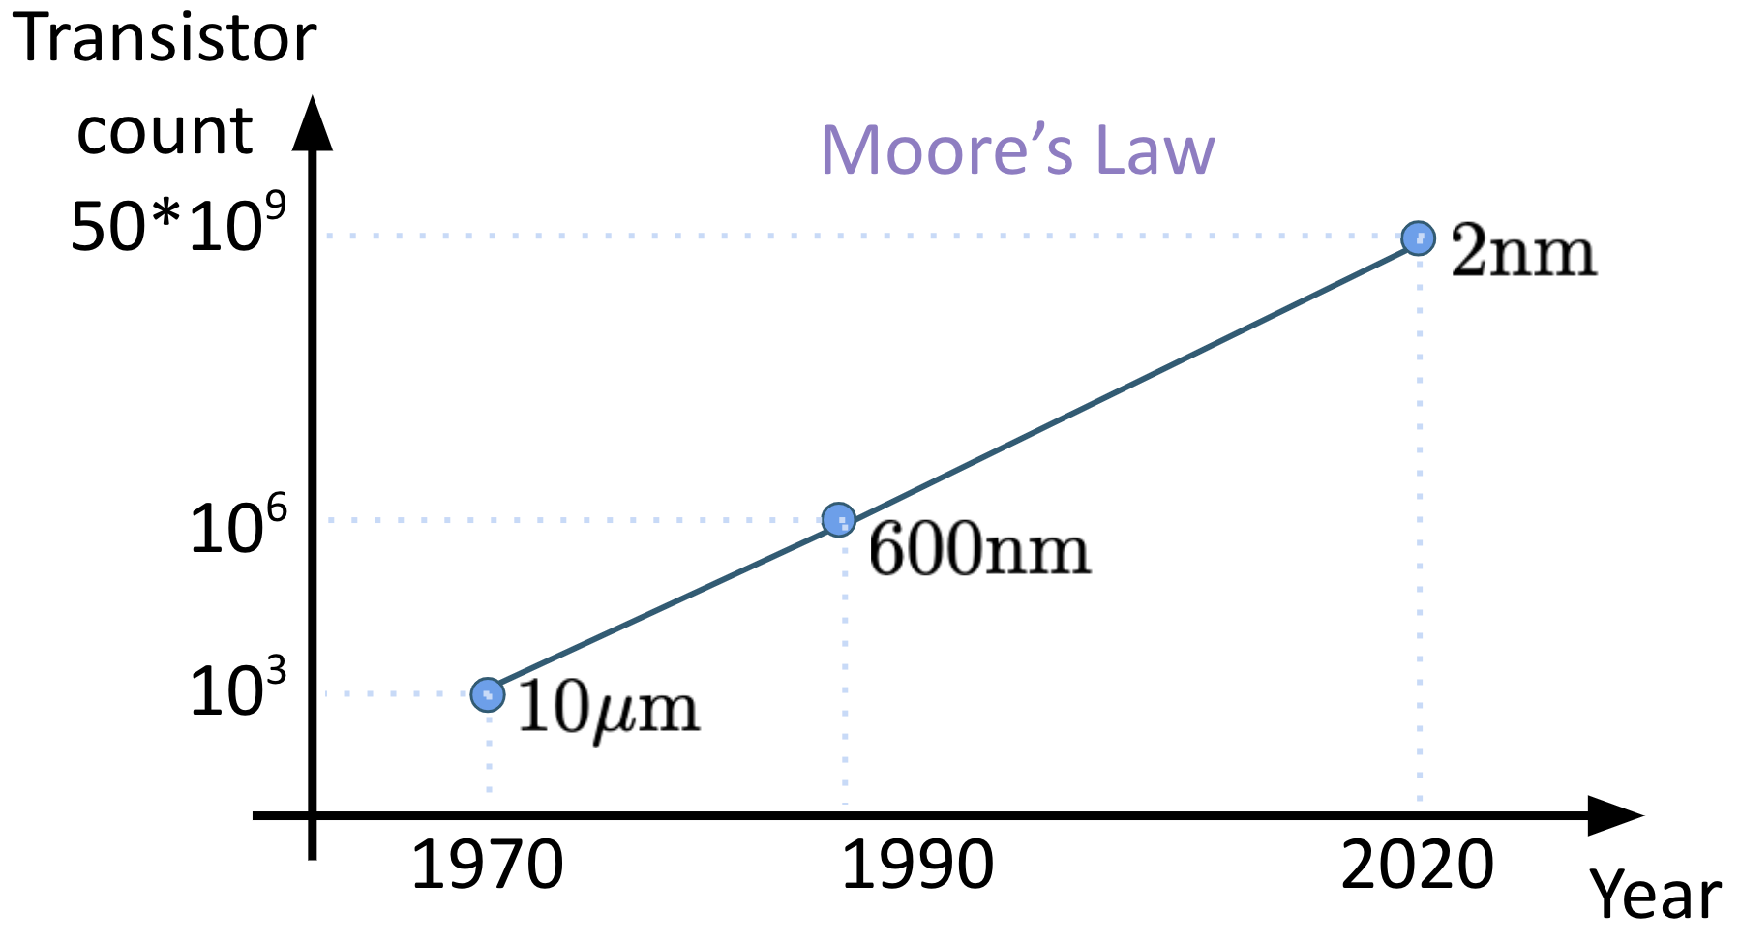
\includegraphics[width=0.8\textwidth]{lesson1/moore_law.pdf}
    \label{fig: 1}
    \begin{center}
        \caption{ムーアの法則}
    \end{center}
\end{figure}
1970年には最初のマイクロプロセッサーができたんですが、
それはインテルの4004のやつなんですが。2300トランジスタが入っていたんですね。すると1990年ぐらいには100個のトランジスタが、一つのチューブに入るようになってたし、2005年ぐらいには、10億トランジスタが入るようになりました。この進化が、\emph{「Moore's Law (ムーアの法則)」}と言いますね。
インテルのファウンダーのゴードン・ムーアさんが、1964年にそれについての論文を提出したんですけれども、「各時期には一つのチップに入るトランジスタの数が倍になるでしょう。」と書いていました。最初の提案は、2年間か3年間なんですが、一番速く進化してた時代には、それが18ヶ月くらいには倍になってたんですね。でもそれが最近は段々その進化が遅れるようになっているんですが。一つの理由としては、そのトランジスタの大きさが変わっているんでしょうね、その技術の進化として。
技術の進化はチップの大きさがあまり変わらないんですね。
時代から時代に進むと。例えば、一つのチップは大体親指の爪ぐらいの面積なんですよね。2cm x 2cmぐらいなんですが、それがさっきの進化の説明した通りで、入るトランジスタの数が増えることなんですが、トランジスタの大きさが段々小さくなるんですよね。その1970年代のトランジスタが、10マイクロメートル(μm)ぐらい。一つのマイクロメートルは1m の100万分の1なんですが。
進化すると、今の時代には、数ナノメートル(nm)。一つのナノメートルが
マイクロメートルの1000分の1ですね。メートル(m)の1000分の1が、ミリメートル(mm) で、ミリメートルの1000分の1がマイクロメートルになって、マイクロメートルの1000分の1がナノメートルになるんですね。

それが続くと、もう一番小さいトランジスタの部分が数ミリしかないんですが、その数ミリの大きさで、\textbf{トランジスタがほぼシリコンの原子の大きさ}ぐらいになっているんですね。シリコンの水晶の中には、原子と原子の距離が0.5ナノメートルぐらいしかなってないなら、2ナノメートルになるなら、それが4個になります。その進化はそろそろ終わってしまうんですよね。それが原子の一個下のトランジスタを作る手法がわからないので。
\subsection{唯一の救世主:量子力学}
すると、量子力学によってどのような新しい展開が生まれるでしょうか?
新しい概念、新しくできることはどのくらい変わるでしょう?
\textbf{重ね合わせ (superposition)}を使うんですが、それが波を使って、その波の特徴を使って重ね合わせの状態のようになることなんです。それは次のレッスンで説明します。True and False (真偽)、On and Off (オンとオフ)
Yes and No(イエスとノー)をそれが表示できるようになるんです。

次の概念が\textbf{エンタングルメント (entanglement)}なんですが、そのエンタングルメントは\textbf{「量子もつれ」}と言いますが、それは古典の場合にはないんで、それが重ね合わせを使って、複数の量子とビットとか使って、離れている距離で重ね合わせを作ると、
それがエンタングルメントになる場合があるんですが、この次のステップで説明します。これが\textbf{Correlation(相関関係)}になるんですけれども、
その相関関係が古典より強くなります。そうすると、新しい通信の手法が生まれます。そうすると、これが量子ネットワークの基底になるんです。それが使えるようになる量子通信を目指しています。
\subsection{まとめ}
さて、この量子通信は難しいんでしょうかね?まあ、すごく壊れやすい状態なんですけれども、それが\textbf{「decoherence(デコーヒレンス)」}と言います。デコーヒレンスは古典のノイズと同じ概念なんですが、それがさっきの話をしてた重ね合わせと量子もつれが破壊される場合があります。そうすると、新しいプロトコルを開発しなければなりません。それが、このモジュールの一つの目的としては、それがどうやって開発されているのかを説明することです。

これが\emph{challenge(挑戦)}かもしれないんですけれども、これが\emph{oppotunity(機会)}にもなりますよね。これが良い機会になるので、量子の特徴を使って新しいシステムを作る事は可能です。これが\emph{interdisciplinary(学際的な、分野を横断した)}ことなんですけれども物理学者も必要だし、数学も必要だし、Electronic Engineers(電気・電子技術者)も必要だし、Computer Scientists(計算機学者)も必要だし、Computer Engineers(計算機技術者)も必要なんですね。



\section{量子時代のセキュリティ}
\subsection{紹介}
量子技術がいろいろな分野に影響するんです。
例えば、
\begin{enumerate}
    \item 材料の科学
    \item 測定の手法
    \item 医療系
    \item 人工知能
    \item
\end{enumerate}
このステップは量子通信についてのテーマですから、セキュリティの方を説明したいと思います。

\subsection{古典通信VS量子通信}
% insert unencrytped msg pic (milk please)
\begin{figure}[H]
    \centering
    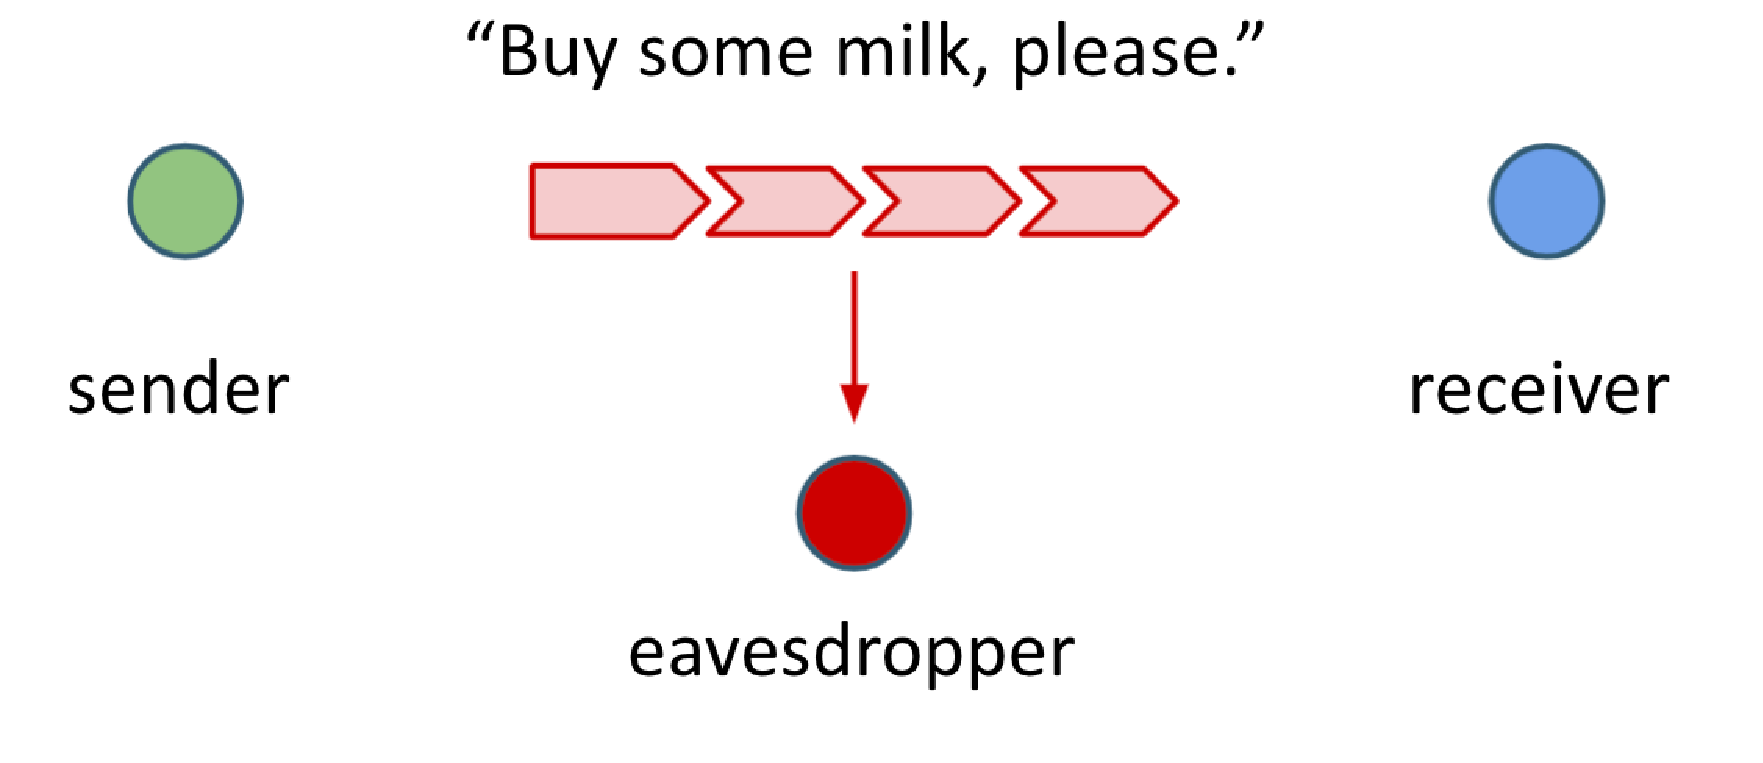
\includegraphics[width=0.8\textwidth]{lesson1/milkplease.pdf}
    \label{fig: 1}
    \begin{center}
        \caption{暗号無しの通信:つまらない内容}
    \end{center}
\end{figure}
まずはメッセージを送りたい状況なんですが、それが暗号されてない場合だったら送信者と受信者がいるんですが、
こういう赤いところは、これは\textbf{チャンネル(通信路)}なんですが、
そのチャンネルにメッセージを通して、盗聴者がいたら、その盗聴者がメッセージをコピーして内容が完全に読めることはできるでしょう。あとは、内容の変更も可能なんですが、この場合のプライバシーについて議論したいと思います。
例えば、メッセージの内容が「牛乳を買ってきてください」とかいうと、
その内容はもしかして誰かがその内容をわかって入れば問題ないかもしれないんですが、他の例にすると、例えば
% insert credit card info 
\begin{figure}[H]
    \centering
    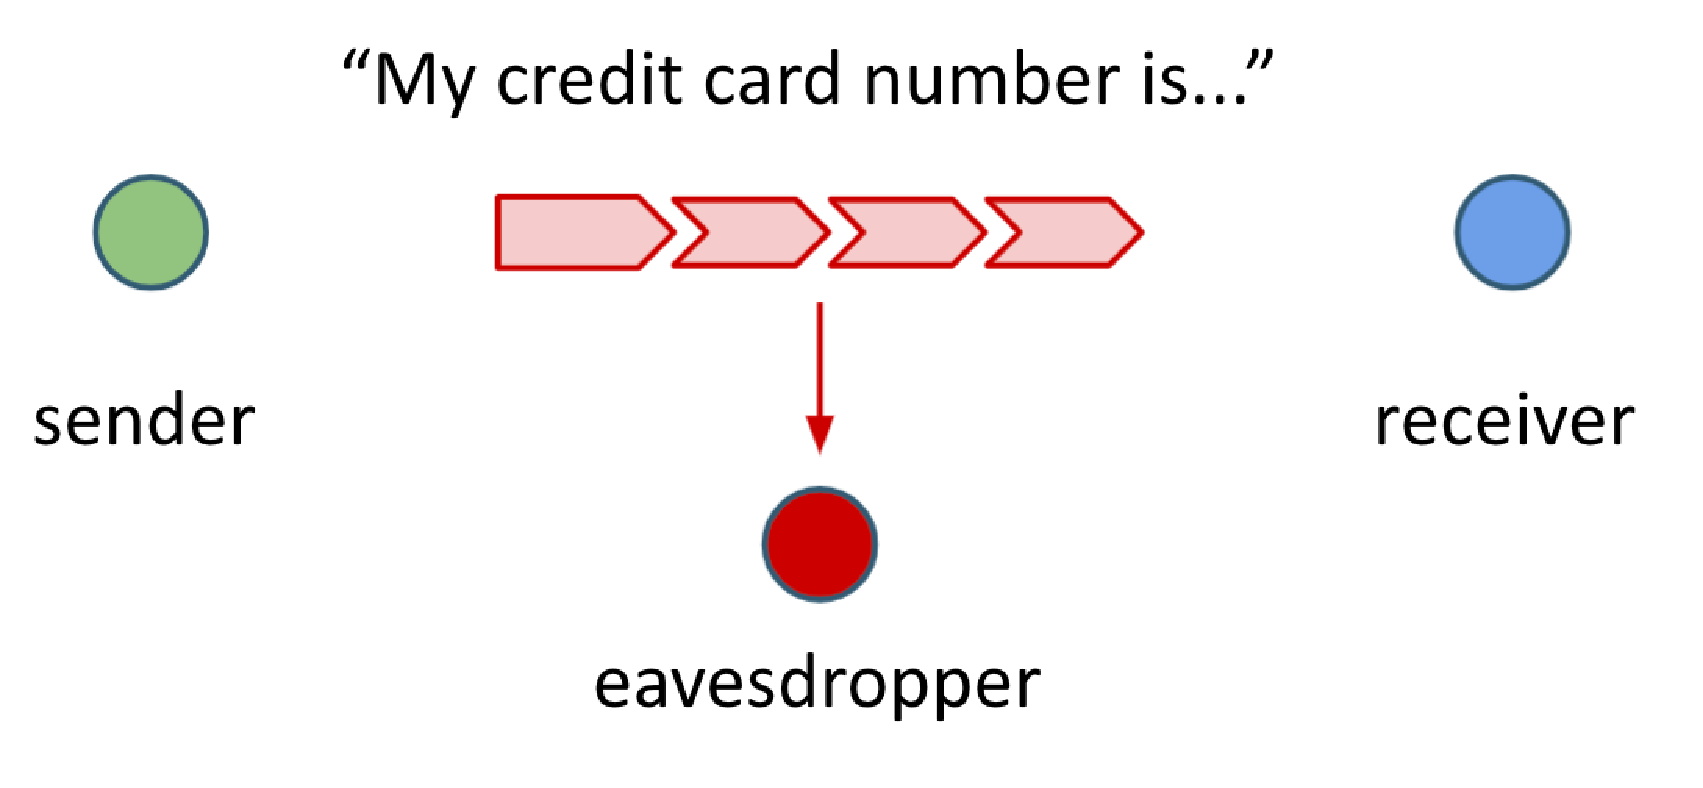
\includegraphics[width=0.8\textwidth]{lesson1/creditcardinfo.pdf}
    \label{fig: 1}
    \begin{center}
        \caption{暗号無しの通信:大事な内容}
    \end{center}
\end{figure}
「僕のクレジットカード番号はこれです」とメッセージを送ってたら、
盗聴者はそれが盗聴したら、そのクレジットカードを使えるようになるかもしれないので、困る場合はありますよね。

さて、これが大きな問題になるかもしれない。
なので暗号が開発されたんですが、その暗号は何千年間の歴史があるんですが、すごく軽く説明をしましょう。
% encrypted msg pic.
\begin{figure}[H]
    \centering
    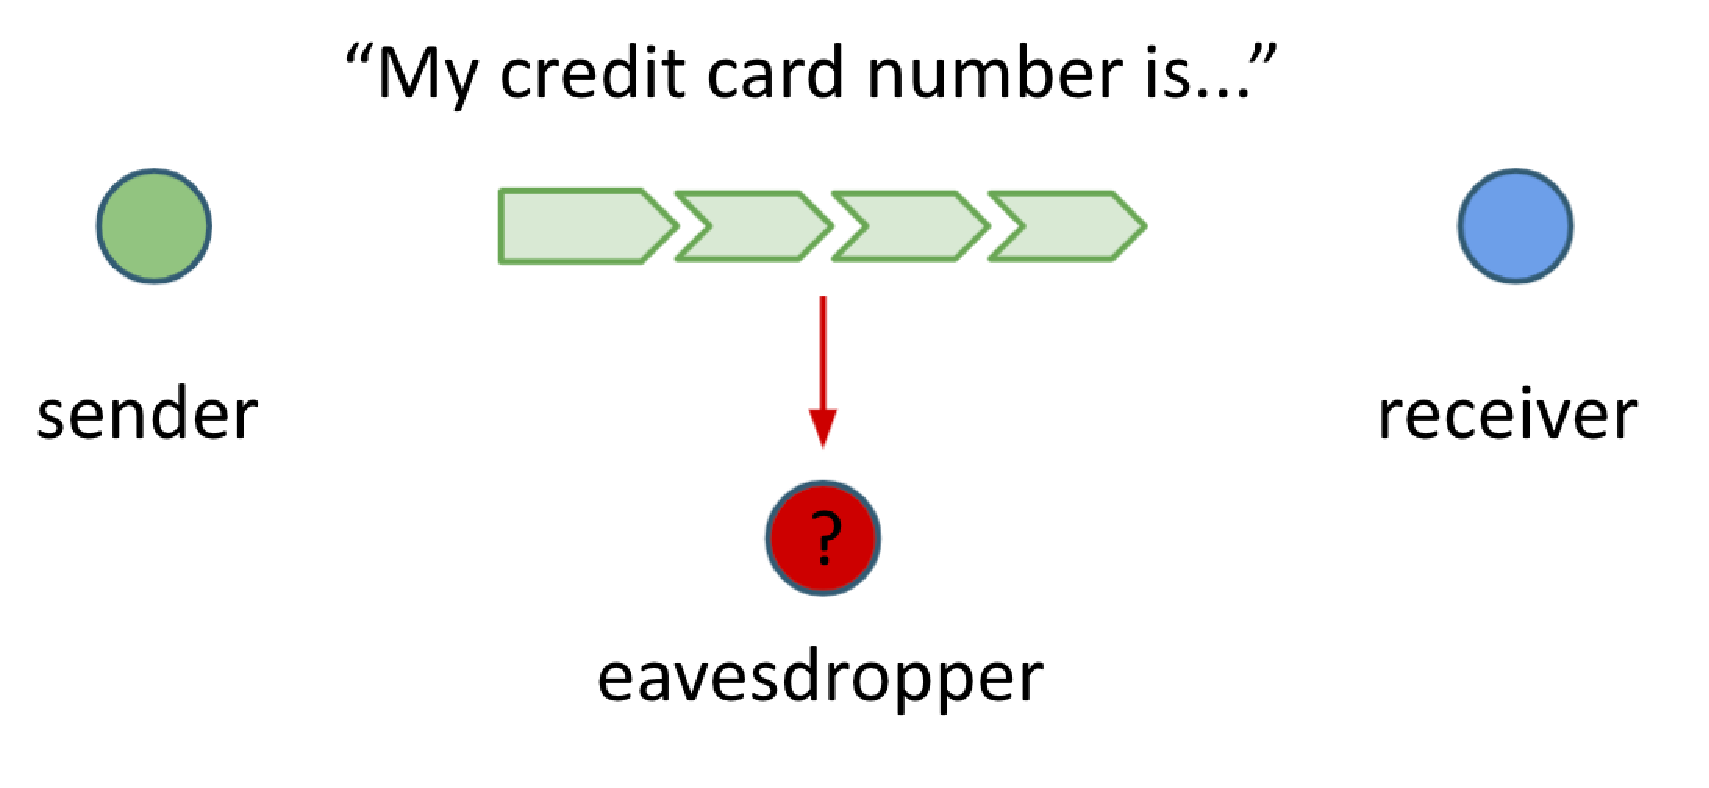
\includegraphics[width=0.8\textwidth]{lesson1/credit_card_info_eavesdropper.pdf}
    \label{fig: 1}
    \begin{center}
        \caption{暗号化された通信}
    \end{center}
\end{figure}
例えば、これだったら送信者から受信者までメッセージ送りたいんですが、その送っているメッセージが暗号化されている場合なら内容は盗聴者は読めないので、安全と言えるでしょう。しかし、それが完全に安全と言えないんですよね。暗号の問題は解読することは不可能ではないんですが、
数学的には問題には関連する指数があるんですが、それ(暗号の問題を)を解決することは難しいんですが、不可能ではない。
解読の手法によるんですが、基本的にはここまで考えてみましょう。
% insecure channel pic.
\begin{figure}[H]
    \centering
    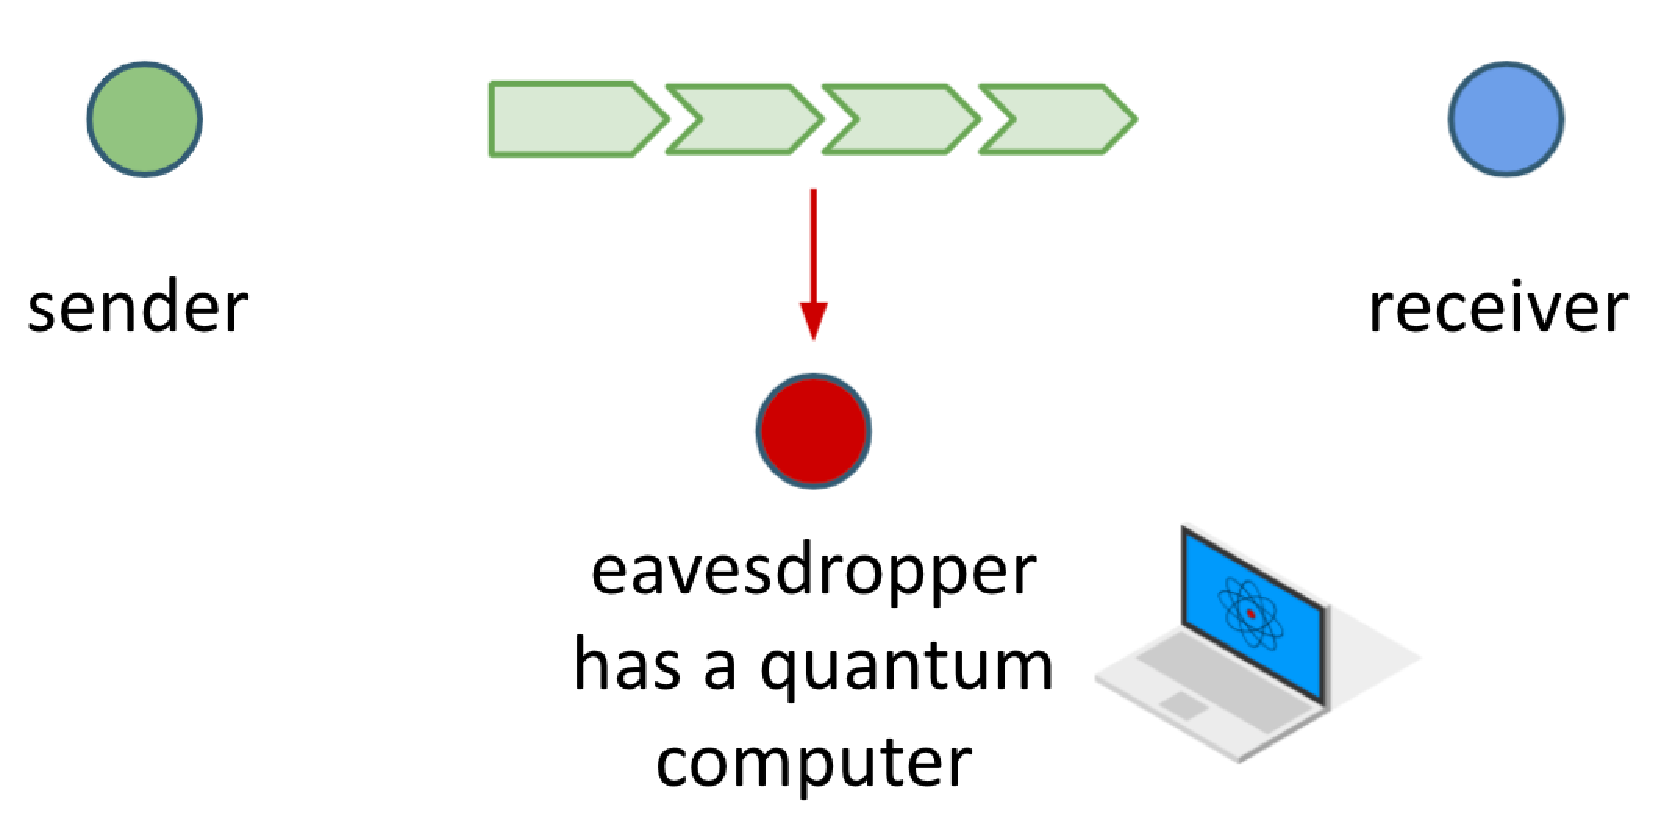
\includegraphics[width=0.8\textwidth]{lesson1/eavesdropper_Q_comp.pdf}
    \label{fig: 1}
    \begin{center}
        \caption{量子コンピューター持つ盗聴者}
    \end{center}
\end{figure}
例えば、その盗聴者が量子コンピュータを使えるなら、数学的な暗号手法を解決する可能性はあるんですが、そうすると例えば、これから勉強することなんですが 、
ディフィー・ヘルマンの鍵交換とかのシステムについては、量子コンピュータが解決する可能性があります。そうすると、このチャンネルがセキュアなチャンネルじゃなくて、インセキュア(安全でない)チャンネルと呼びましょう
量子チャンネルを使っていたら、 量子コンピュータじゃなくて、

このチャンネルを量子チャンネルに変更したらある手法を量子暗号、量子鍵交換の技術を使ってたら解読は不可能にはなるんですが、盗聴者がいるかどうかは重要なメッセージを送る前に発見することは可能です。
% Quantum Channel "STOP" pic
\begin{figure}[H]
    \centering
    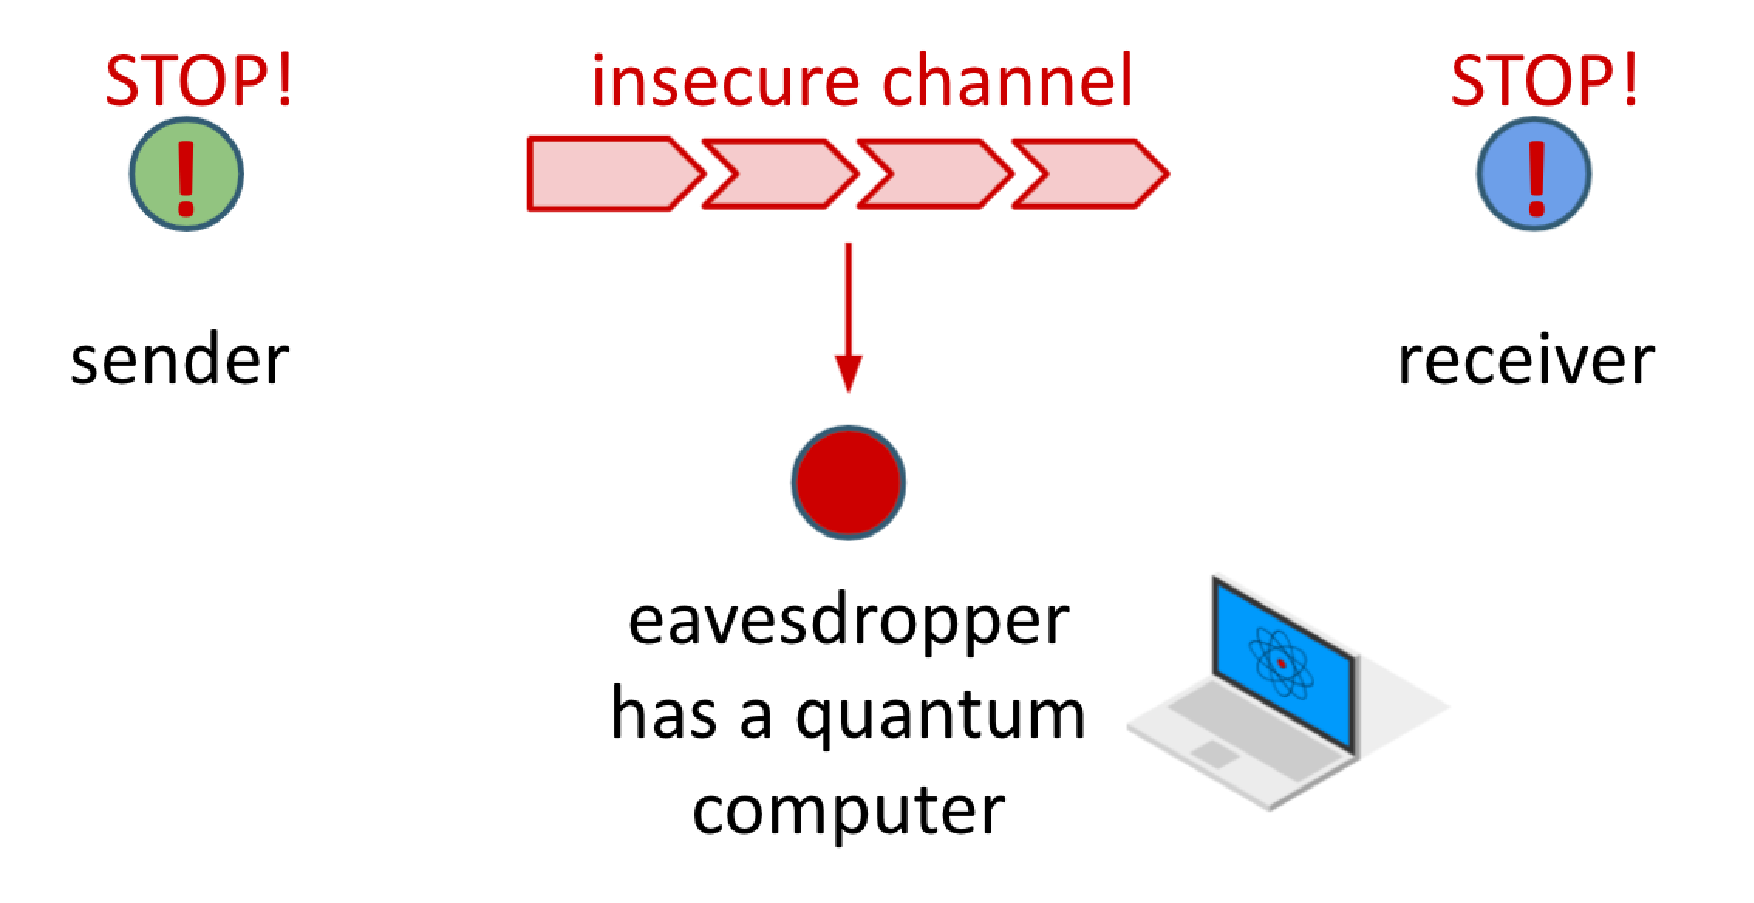
\includegraphics[width=0.8\textwidth]{lesson1/insecure_channel_stop.pdf}
    \label{fig: 1}
    \begin{center}
        \caption{量子チャンネル:通信中止}
    \end{center}
\end{figure}
送信者と受信者は盗聴者がいることがわかるようになります。盗聴者の存在に気付く送信者と受信者はその通信を止めることができます。


\section{モジュールの概要}


今学期には何を勉強するでしょう。
% insert course overview pic
\begin{figure}[H]
    \centering
    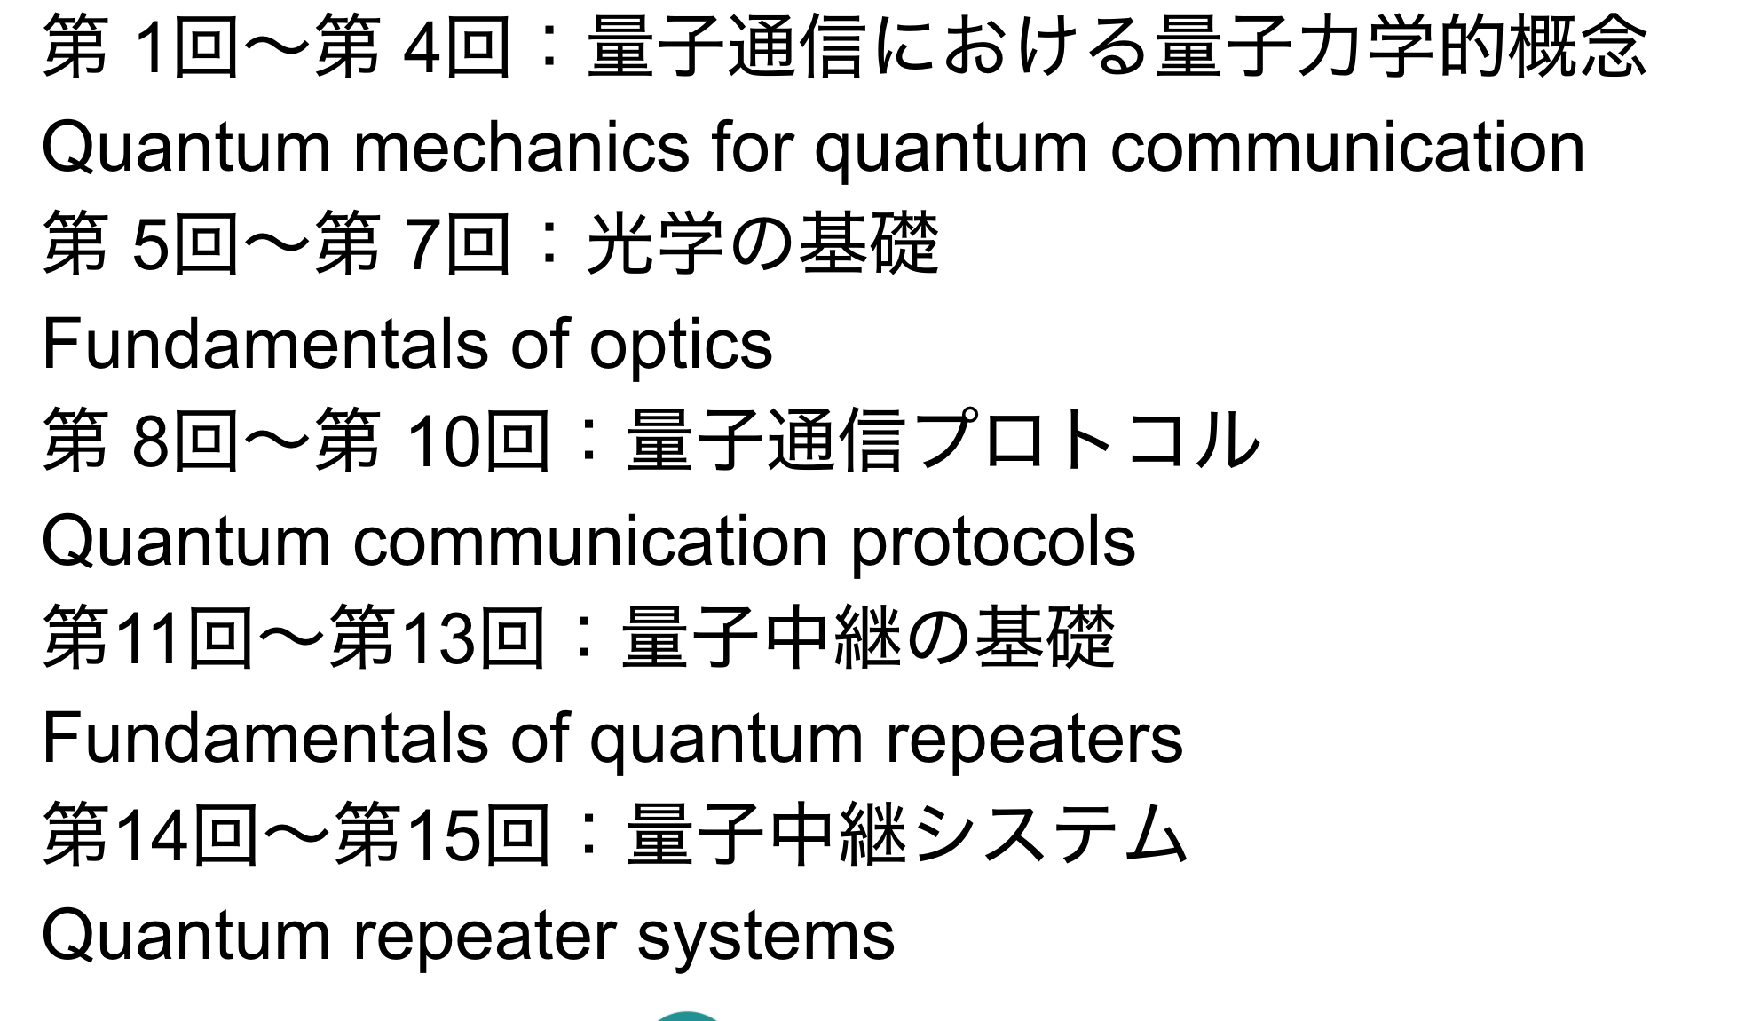
\includegraphics[width=0.8\textwidth]{lesson1/module_overview.pdf}
    \label{fig: 1}
    \begin{center}
        \caption{モジュールの概要}
    \end{center}
\end{figure}
このモジュールにはいくつかのテーマが
あるんですけれども、1、2、3、4、5のテーマに分けているんです。
レッスン1から4までは量子力学なんですが、深くは勉強しないんですが軽く紹介することとしています。レッスン5から7までは、光学の基礎なんですが、レッスン8から10は、量子通信の基礎。それは量子鍵配送等を含むことです。レッスン11から13は、量子リピーター、量子中継器の基礎なんですが、14と15はその量子中継器のシステムについて議論します。
\subsection{前提について}
% insert pre-requisities slide 
\begin{figure}[H]
    \centering
    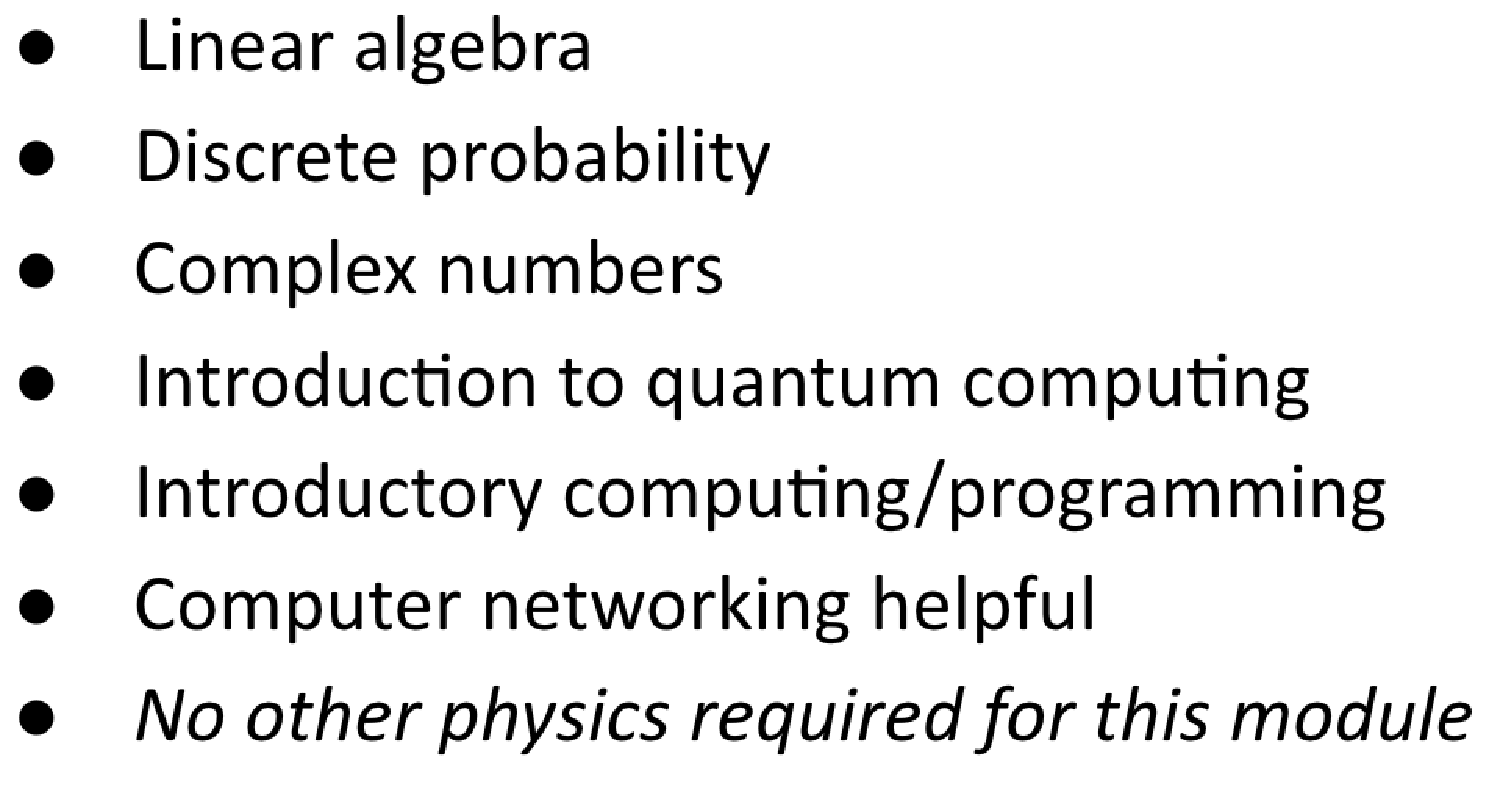
\includegraphics[width=0.8\textwidth]{lesson1/prereqs.pdf}
    \label{fig: 1}
    \begin{center}
        \caption{コースの前提}
    \end{center}
\end{figure}
これは何を前提としているのでしょう?前提か、一緒に勉強しているのか、
進みながらもできることにはできると思うんですがまずは\emph{線形代数}。それがすごく重要なんです。あとは、\emph{確率}。これが簡単な方だけなんですが。あとは、\emph{複素数}。それも、\emph{オイラーの方程式}も重要なんです。あとは、並列で\emph{量子計算の基礎}を勉強した方がいいと思います。これがコンピューティングシステムズの内容なので、
基本的にプログラミングができることも重要だと思います。\emph{Pythonの言語}は、ちょっとだけは使うことにはするんです。
そして普通の\emph{古典コンピューターネットワーク}も重要なんです。
インターネットとかTCP/IPとかネットワークの基礎のことを勉強するということは重要。それから、物理学はあんまり内容は深くはしませんが、
重要な量子力学は最初の方には説明するのですが、
それ以外は、特別な物理学の授業を履修しなくても結構です。

さて、その量子計算機の入門としては、いくつかのオプションがあるんですけれど一つは、慶應大学の開発した「Understanding Quantum Computers
(量子コンピュータの理解)」のMOOC。オンラインコースで、これが高校生レベルから学部の1年生あたりのレベルなんですが、数学はあまり使ってなくて、最初のものは英語なんですが、日本語、タイ語、インドネシア語の字幕と記事もそれらの言語に翻訳されているものがありますから、安心して使ってください。

% Rod videos pic
\begin{figure}[H]
    \centering
    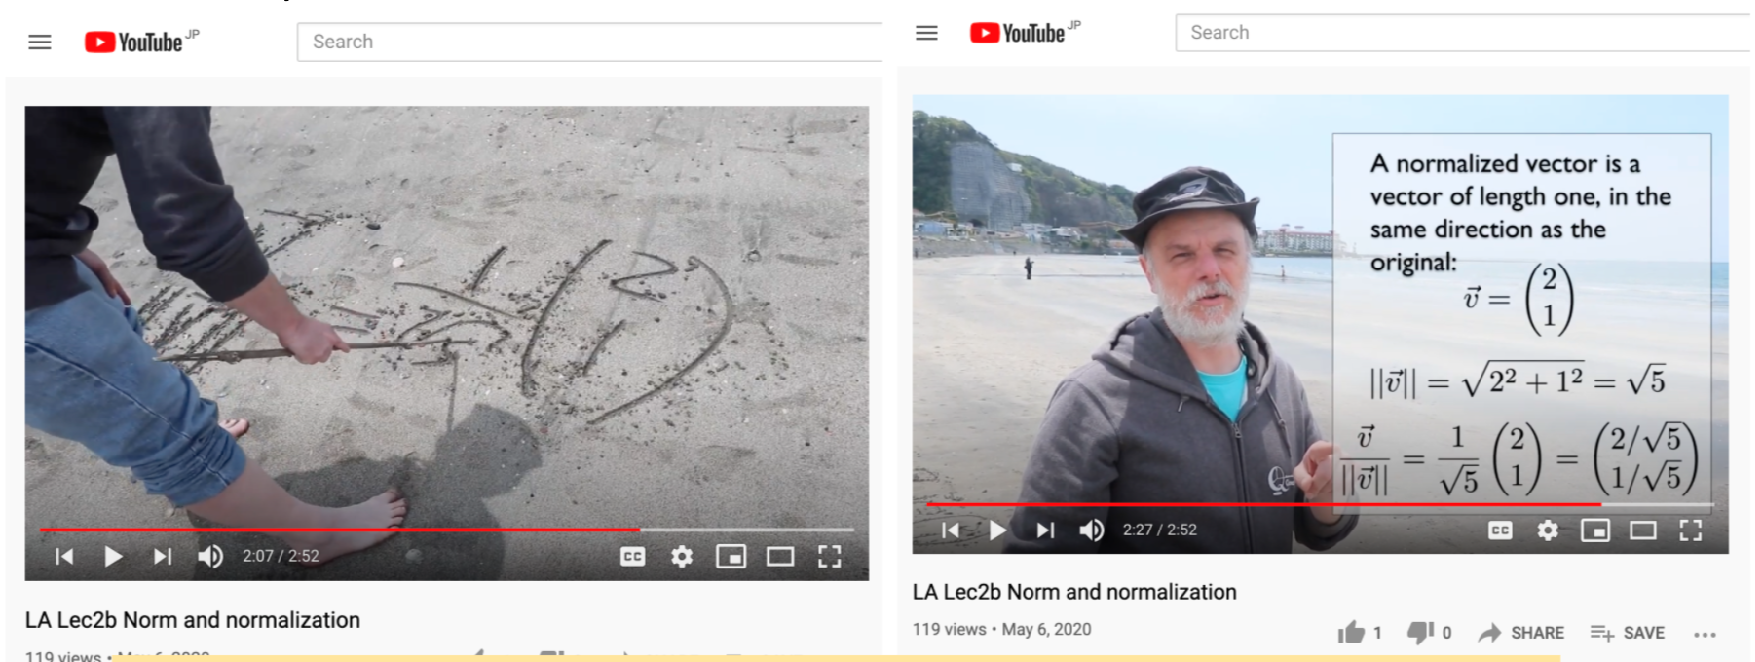
\includegraphics[width=1.1\textwidth]{lesson1/lin_alg_vids.pdf}
    \label{fig: 1}
    \begin{center}
        \caption{先生の線形代数ビデオ}
    \end{center}
\end{figure}

さて、線形代数としては、それもいろんなところで学べるのですが、
他の選択肢がないなら、慶應大学の湘南藤沢キャンパスで線形代数の授業は
そのビデオが、Youtube にアップされてますので、こちらのURLでアクセスしてください:
\url{http://www.youtube.com/playlist?list=PLibMrvP9xUbeWZ1pCKnbTn2FO-c1PqHZr}.

大体はこの内容なんですが、もちろんそれをやりながら見えてくるんですけれども、これから量子通信の基礎を楽しくワクワク勉強しましょう!

\chapter[量子状態]
\chapter{量子状態}


% \chaptermark{Environmental Policy Analysis with STREAM}

%\chapterauthor{Hein Mannaerts}



\begin{abstract}
Lesson abstract goes here
\end{abstract}


\section{量子ビット}
古典ビットだったら二つの状況が可能です。ビットは0か1になる。0だったらそれが100\%0だと言えます。1だったらそれが100\%1だと言えます。
% Insert qubit 100% 0
\begin{figure}[H]
    \centering
    \includegraphics[width=0.8\textwidth]{lesson2/100%0.pdf}
    \label{fig: 1}
    \begin{center}
        \caption{100\%0 キュービット}
    \end{center}
\end{figure}
量子ビットだったら\textbf{「キュービット」}と呼びますが0の状態と1の状態がありますがそれが、100\%0の状態の時もあります。その場合、この記号の中に書きます。アングルブラケット(角括弧)の中に書きます。
% Insert qubit 100% 1 
\begin{figure}[H]
    \centering
    
\includegraphics[width=0.8\textwidth]{lesson2/100_1.pdf}
    \label{fig: 1}
    \begin{center}
        \caption{100\%1 キュービット}
    \end{center}
\end{figure}
もし1の状態だったら1をアングルブラケットの中に書きます。100\%1の状態の時に
ですが、それだけじゃなく\emph{その間の状態}も可能です。
% Insert superposition state pic.
\begin{figure}[H]
    \centering
    
\includegraphics[width=0.8\textwidth]{lesson2/superposition_qubit.pdf}
    \label{fig: 1}
    \begin{center}
        \caption{重ね合わせ状態キュービット}
    \end{center}
\end{figure}
例えば50\%0の状態プラス50\%1の状態。その場合、この様に書きます。これを\textbf{重ね合わせ}と言います。この重ね合わせの状況は古典のビットにはできないですよね。
この記号この書き方をもう少し説明しましょう。
\begin{equation}
\ket{\psi} = \alpha \ket{0} + \beta\ket{1} 
\end{equation}
これは、\textbf{ディラックノーテーション}と言います。この左側に書いてある状態は$\psi$ (\emph{psi}) の状態と言いますが、(\emph{alpha}) かける0プラス\emph{beta}かける1と読みます。
% Dirac Notation w/ annotation
\begin{figure}[H]
    \centering
    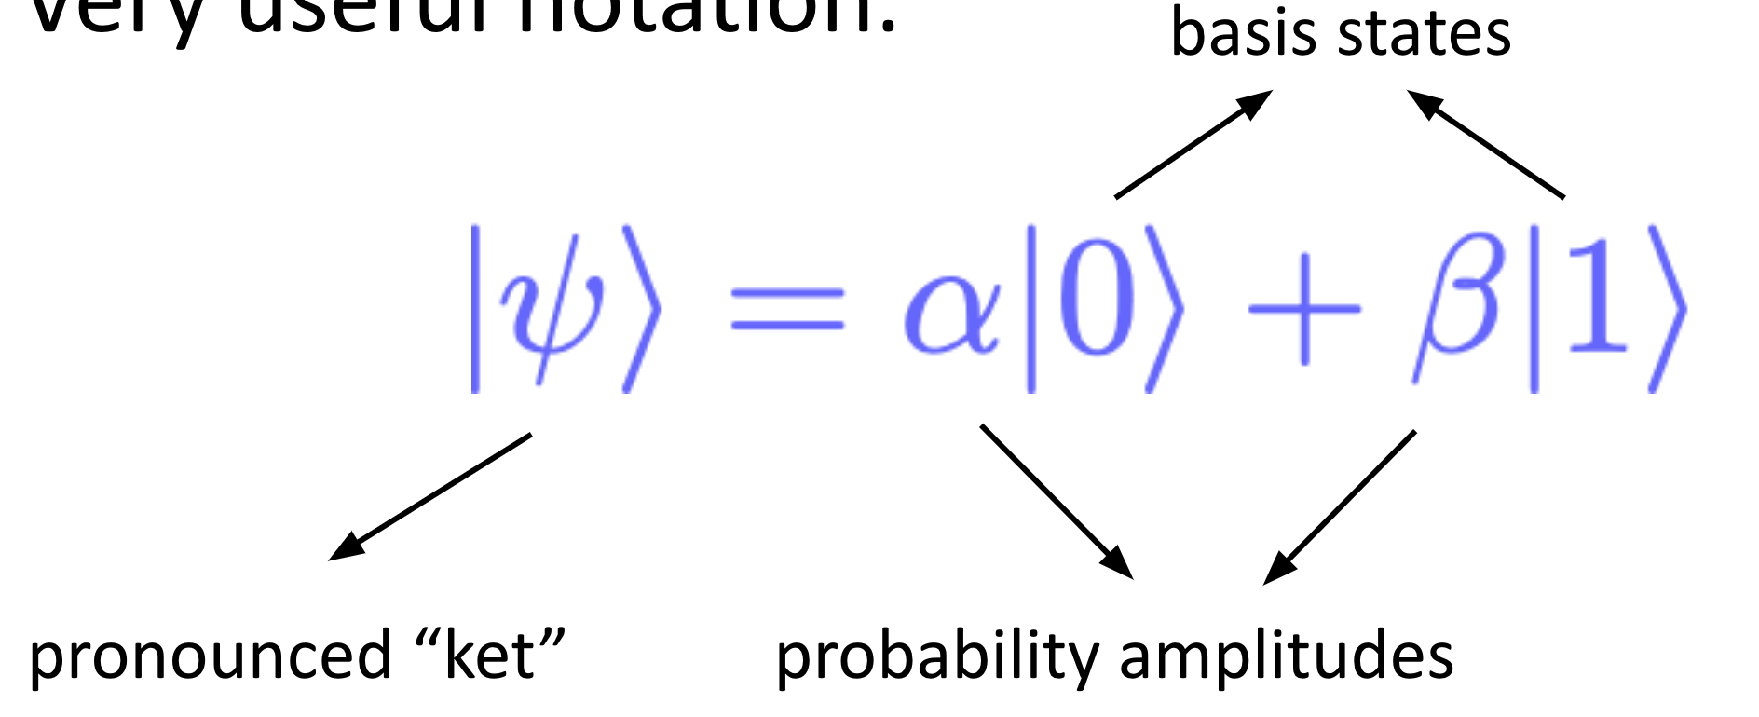
\includegraphics[width=0.8\textwidth]{lesson2/dirac_notation.pdf}
    \label{fig: 1}
    \begin{center}
        \caption{ディラックノーテーション}
    \end{center}
\end{figure}
$\psi$, 0, 1 を囲むのは\textbf{ケットノーテーション}と言います。これがケット記号。この0と1は\textbf{basis state}、つまり基底ベクトルです。この$\alpha$と$\beta$は\textbf{probability amplitudes}、つまり、確率振幅です。 これは複素数になることが可能です。これは正規化しなければならになりませんので、絶対$\alpha$の二乗足す絶対$\beta$ の二乗 が1に等しくなければなりません。
% Bloch Sphere
\begin{figure}[H]
    \centering
    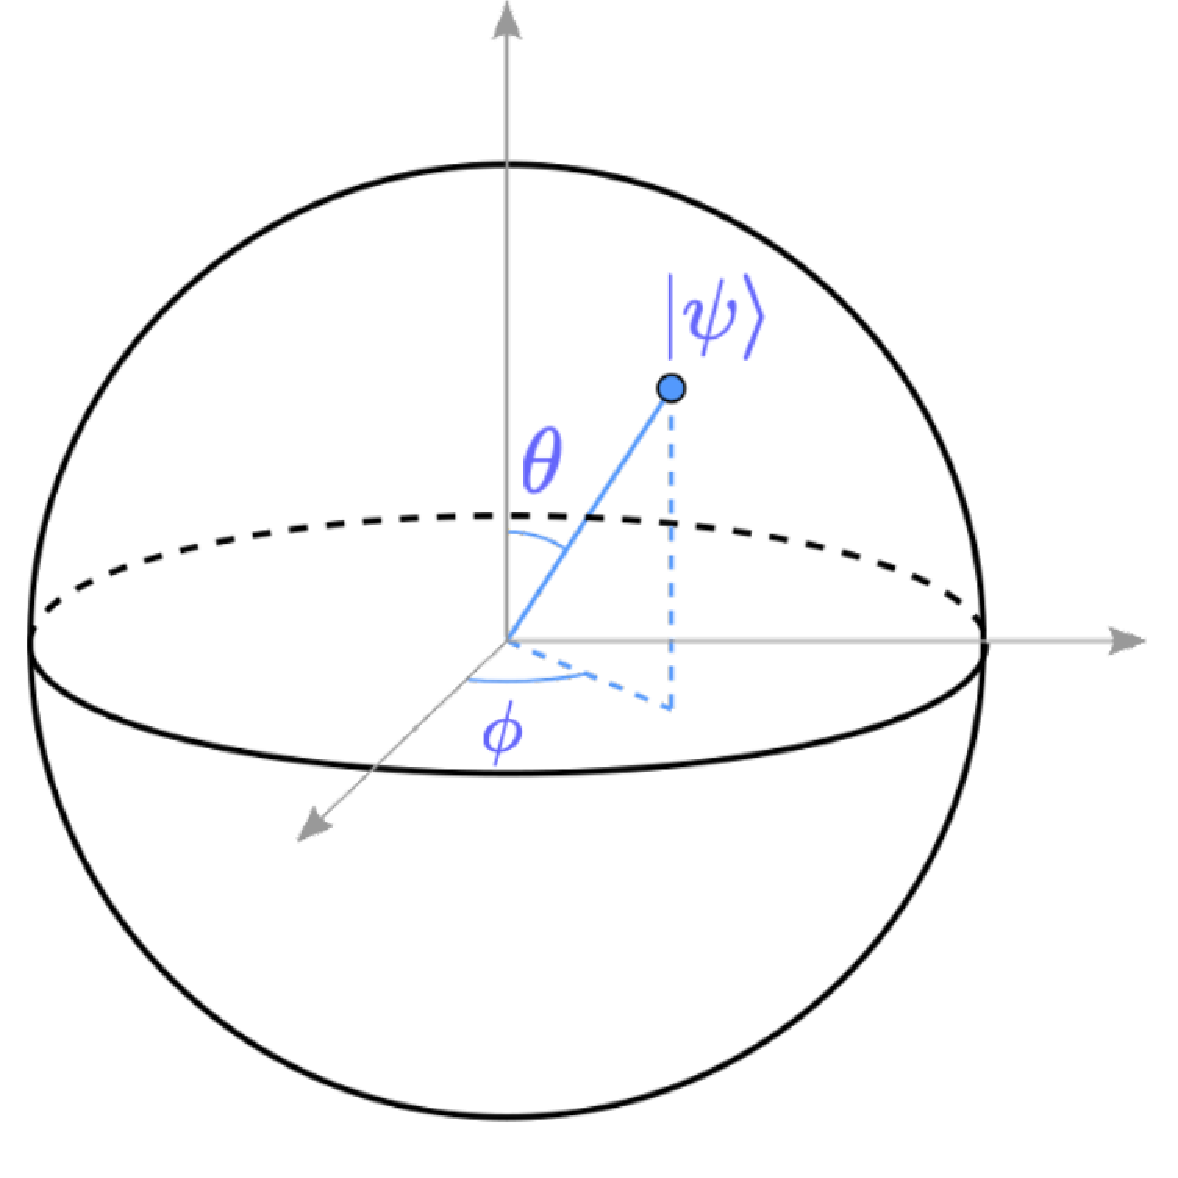
\includegraphics[width=0.6\textwidth]{lesson2/bloch_sphere.pdf}
    \label{fig: 1}
    \begin{center}
        \caption{ブロッホ球}
    \end{center}
\end{figure}
もう一つの表示の仕方としては\textbf{ブロッホ球}があります。このブロッホ球は1つの量子ビットの状態を表示できます。これは2つの角度を使うんですが、
$\theta$の角度と$\phi$の角度でこの$\psi$の状態を書きます。そうするとこの$\psi$の状態は次のように表せます。
\begin{equation}
|\psi\rangle=\cos \frac{\theta}{2}|0\rangle+e^{i \phi} \sin \frac{\theta}{2}|1\rangle
\end{equation}

この$e^{i\phi}$は\textbf{phase}、あるいは位相と言います。これは一つの量子ビットは二つの角度で定義できますがもう一つの言い方をすると三次元の球なのでX軸、Y軸、Z軸を使います。
% insert Bloch sphere w/ axes labelled and |+> |-> meanings
\begin{figure}[H]
    \centering
    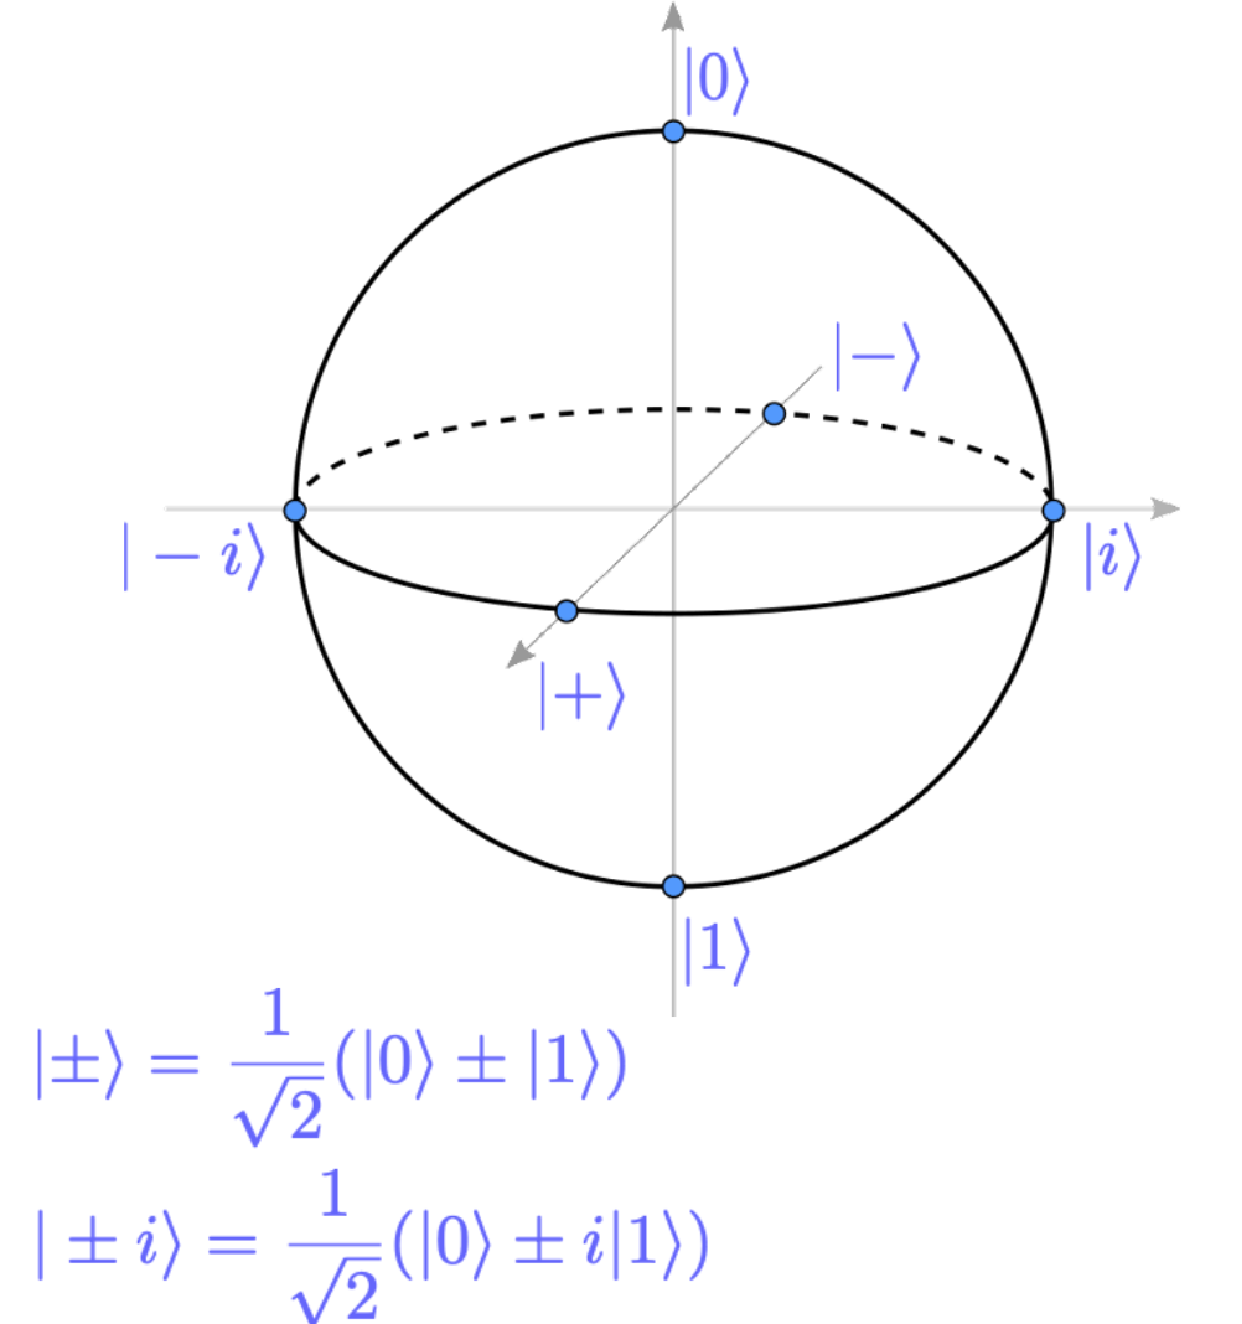
\includegraphics[width=0.7\textwidth]{lesson2/bloch_sphere_annotated.pdf}
    \label{fig: 1}
    \begin{center}
        \caption{ブロッホ球 軸解説}
    \end{center}
\end{figure}
このZ軸は縦の所で0の状態はブロッホ球の一番上の所。1の状態はブロッホ球の一番下の所にあります。そうすると、X軸は赤道にありますがその赤道は前と後ろの方に別れています。前の方の所を+( プラス)の状態と言います。後ろの所を-(マイナス)の状態と言います。なぜこれが+と-の状態と言うのかはこういう風に書くから。0と1じゃなくてこのket notationの中には+と-のを書きます。そうするとこれは、0+1の状態。あるいは0-1の状態になりますすると正規化しなければなりませんので$\sqrt{\frac{1}{2}}$をかけます。そうすると正規化できるでしょう。

続いて、Yの軸の場合+iと-iと言います。それがさっきの所の$\phi$の角度でこれは位相が変更されます。状態を書きますと、さっきと同じ+と-の状態で0+1のなんですけど、間は0と+だけじゃなくて、かけるiになります。これはさっきの位相です。
そうすると、これが+-iの状態で、それがY軸の右と左の所になります。これは一つの量子ビットだけなんで複数の量子ビットには使えない表示の仕方です。


\section{ユニタリ演算}
情報を処理すると何かの物理的なシステムを使います。
% Classical (SSD) VS Quantum (Ion Trap)
\begin{figure}[H]
    \centering
    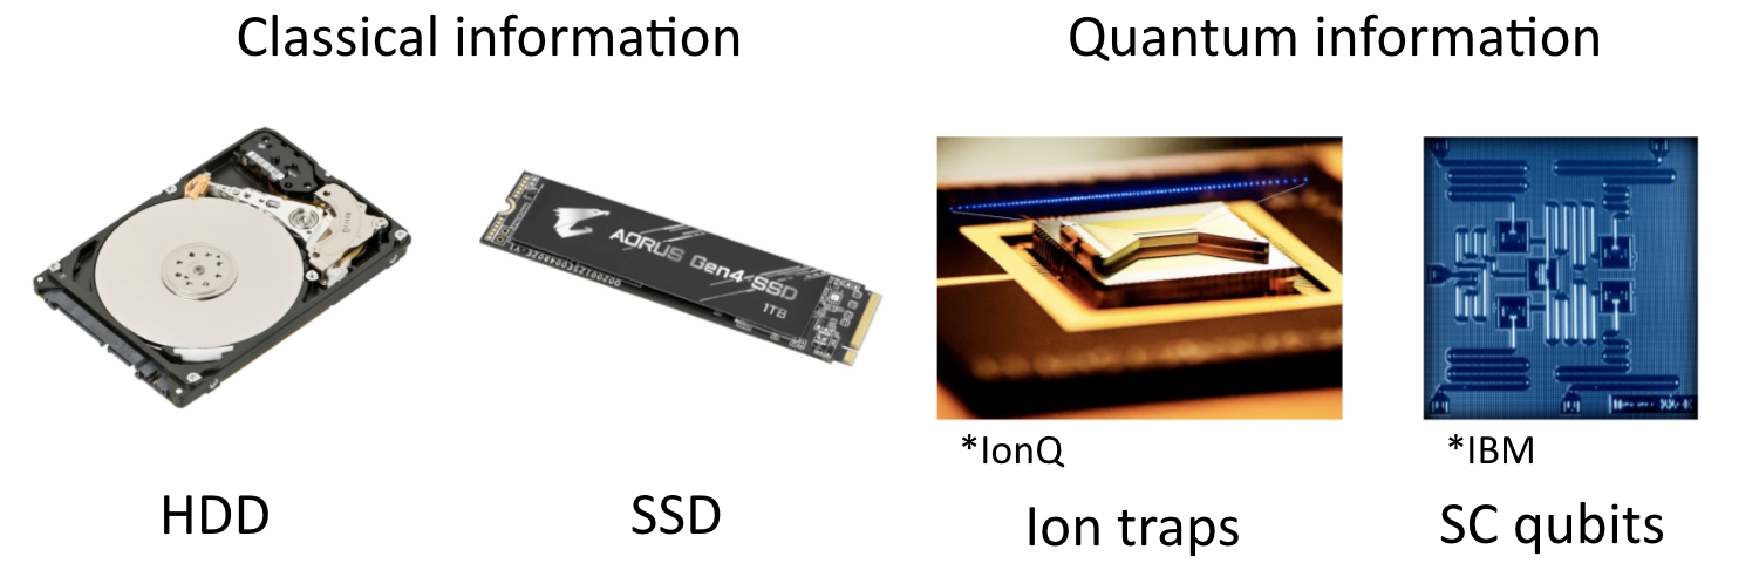
\includegraphics[width=0.7\textwidth]{lesson2/ion_trap_etc.pdf}
    \label{fig: 1}
    \begin{center}
        \caption{物理的なシステム}
    \end{center}
\end{figure}
それは例えば物理のシステムを相互作用しなければなりませんが例えば古典の場合だったら磁気ディスクにデータを保存することも可能性ですしSolid State Driveにもデータを保存することが可能です。これが物理的にはビットの効果で出来ているんですが量子の場合だったら量子情報は例えばこの左側の真ん中のところには
イオントラップがあります。このイオントラップの中にはチップ型の物の上に原子が一個ずつ浮かびます。原子が量子ビットを表示する。その量子ビットを作用すると
計算ができる様になります。例えば右側のは超伝導のチップ、これはIBMの例なんですが、これも量子伝導という量子効果を使ってこれに量子作用による量子影響が起こるとこれが
データを表示してデータを処理できる様になります。これを数学的にも見てみましょう。
\subsection{いくつかの演算}
% Simple Unitary Operations 
\begin{figure}[H]
    \centering
    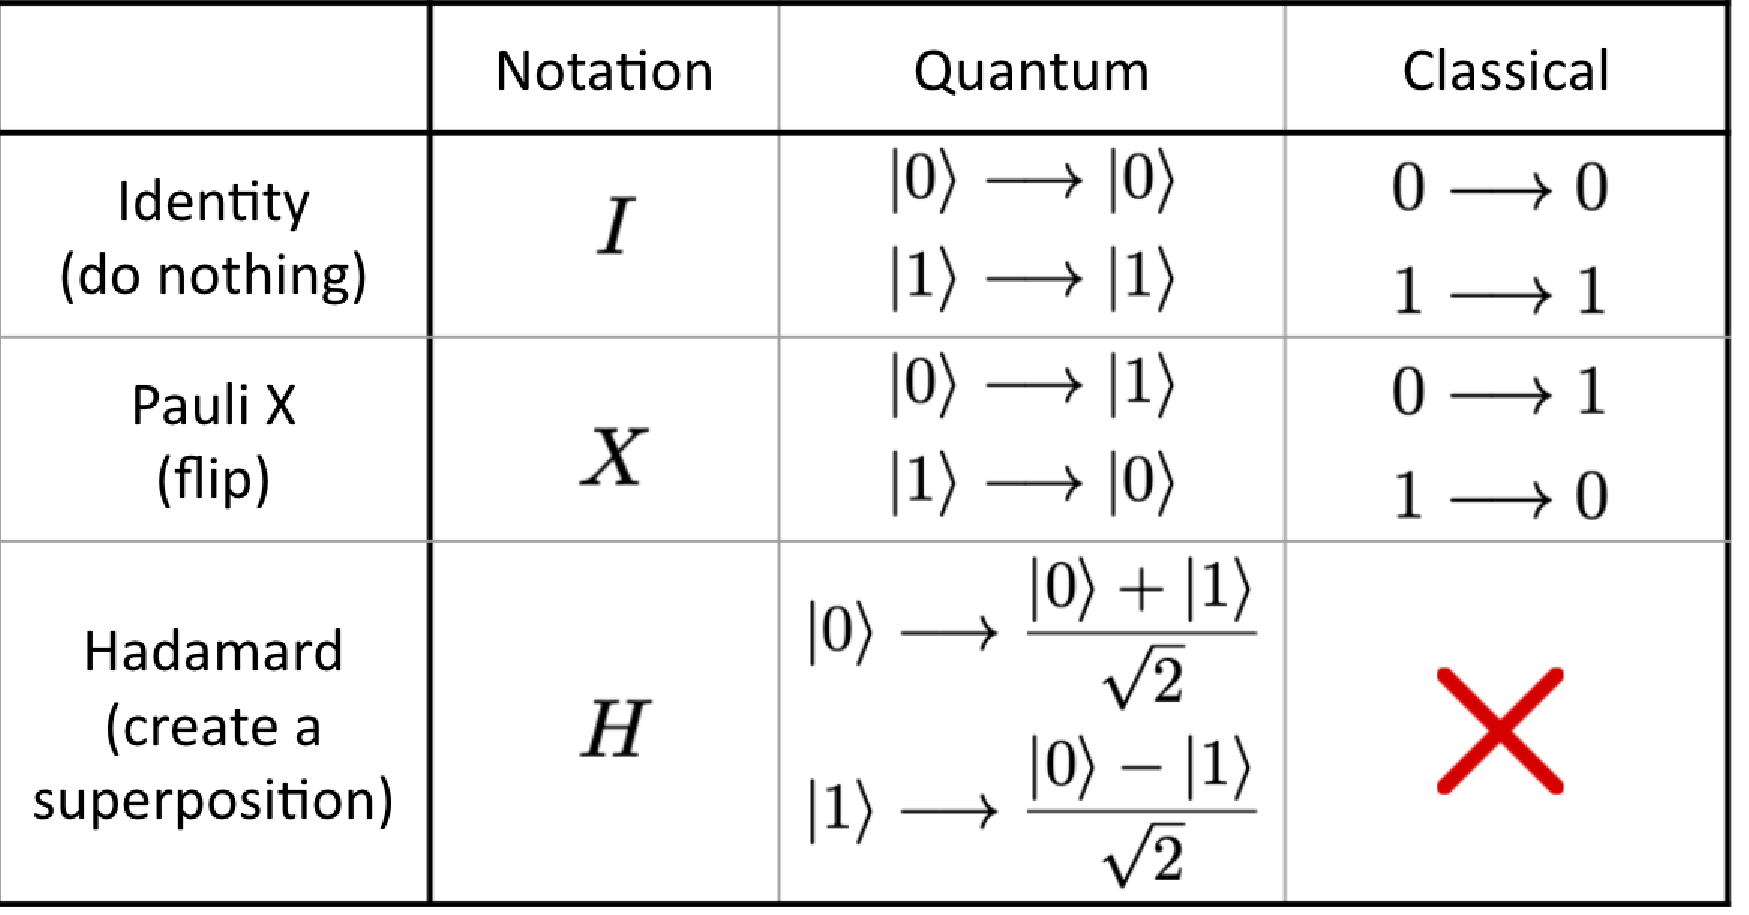
\includegraphics[width=0.7\textwidth]{lesson2/simple_unitary_ops.pdf}
    \label{fig: 1}
    \begin{center}
        \caption{シンプルユニたり演算}
    \end{center}
\end{figure}
まずはこれをユニタリ演算と言いますが例えば一番最初に学ぶのはI(アイデンティティ行列)。このアイデンティティ行列は単位行列です。右側の所には古典(classical)のデータの処理がIdentity Matrixを通ると0のinput stateはそのまま0になり1のinput stateもそのまま1になります。量子の場合だったら一緒で0の状態をinputしたら0の状態がoutputされます。1の状態をinputしたら1の状態がoutputされます。つまり、何も計算せず何も変わらない。これをデータ保存とも言える。

もう一つの例としてパウリ行列のXがありますXの場合は大文字のXで書く。これが\textbf{パウリXユニタリ演算}と言います。これがbit flipになりますそのbit flipというのは古典の場合0が1になり1が0になる。古典の場合これをNotとも言う。
量子の状態でも0の状態をinputしたら1の状態が出てきます。1の状態を入れたら0の状態が出てきます。これも一緒でNotとも言えますが量子の場合だとXゲートあるいはX演算と言います。

もう一つの例として\textbf{Hadamardゲート}があります。Hadamard演算ですがこれは大文字のHを書きます。Hの他の使い方もありますがここではHadamardという意味ですね。Hの場合inputが0だった時outputは0足す1の重ね合わせこれがさっきのステップで言っていた様に正規化もしなければいけないので割る$1/\sqrt{2}$にします。
1のinputをしたら1と0の重ね合わせの結果が出てくる。このoutputの場合位相も違い+ではなく-になる。これも正規化するために割る√2しなければならない。このゲートがこのユニタリ演算は重ね合わせを作る基本の演算となります。この場合古典のデータだと重ね合わせというのはないので古典の場合ありません。
\subsection{ユニたり演算}
さて先程はユニタリ演算という言葉を使っていましたがユニタリ演算て何でしょう?
まあユニタリ演算というのは逆計算が可能な演算です。その逆計算を\textbf{adjoint}と言います。adjointと言うのは随伴です.書くとUが最初の演算だったら$U^{\dagger}$と記号、dagger(短剣符)を使って随伴と言う。そうするとinput stateは$\psi$のケットの場合$U$の演算を掛けると$\psi^\prime$の結果が出て$U^{\dagger}$を掛けると$\psi$の状態に戻る。これは逆計算が可能になっているでしょう。
最初は$\psi$の状況だったが何かを計算し変更されてもう一回やることでoutputと
inputの状態が同じになったので逆計算ができ、これが随伴この$\psi^\prime$という状態が$U$掛ける最初のinputの$\psi$のstateで、$\psi$も$U^{\dagger}$掛ける$\psi^\prime$の状態になるんです。

ちょっと数学的にやってみると$\psi$の状態を
\begin{equation}
|\psi\rangle=U^{\dagger}\left|\psi^{\prime}\right\rangle=U^{\dagger} U|\psi\rangle
\end{equation} 
これは最初の$\psi$と最後の$\psi$が等しくなるためにはこの$U^{\dagger} U$は$I$(アイデンティティ行列)にしなければならない。もう一つの計算手法としては$\psi^{\prime}$にすると
\begin{equation}
\left|\psi^{\prime}\right\rangle=U|\psi\rangle=U U^{\dagger}\left|\psi^{\prime}\right\rangle
\end{equation}
これは最初の$\psi^{\prime}$と最後の$\psi^{\prime}$が等しくなるために$UU^{\dagger} = I$ なので
\begin{equation}
U U^{\dagger}=U^{\dagger} U=I
\end{equation}
でこれはこの演算も行列なのでこれは随伴行列と言います。(adjoint operator, adjoint matrix)。
\subsection{行列表示}
もう少し行列の話をすると状態をベクトルで表示することができますがユニタリ演算は行列で表示します。例えば状態をちょっと見てみましょう。0の状態を古典と同じ様に0と1を使ってるんですが量子の0の状態を使うとこれが本当は
\begin{equation}
|0\rangle=\left(\begin{array}{l}
1 \\
0
\end{array}\right)
\end{equation}
ベクトルとしては$1, 0$の二次元の状態となる。1の状態だったらこれも同様に
\begin{equation}
|1\rangle=\left(\begin{array}{l}
0 \\
1
\end{array}\right)
\end{equation}
二次元のベクトルで1, 0じゃなくて0, 1になります。そして、一つの量子ビットの状態を表示するためには$\psi$と言いますが
\begin{equation}
|\psi\rangle=\alpha\left(\begin{array}{l}
1 \\
0
\end{array}\right)+\beta\left(\begin{array}{l}
0 \\
1
\end{array}\right)=\left(\begin{array}{l}
\alpha \\
\beta
\end{array}\right)
\end{equation}になりますね。

これもベクトルで1つの量子ビットの状態を表示できる様になる。後で$\psi$の変数としては色んな使い方で使いますが今の場合は1量子ビットだけです。

するとさっき言ってたIのoperatorが行列で書かなければけませんが

0:09:00.483,0:09:05.411
これは
\begin{equation}
I=\left(\begin{array}{ll}
1 & 0 \\
0 & 1
\end{array}\right)
\end{equation}
の行列で斜めの所は全て1なので\textbf{diagonal, diagonal}じゃない所は全部0になる行列になります。これは2掛ける2の行列ですがもっと大きいやつもできます。それとこれからよく使う行列は三つあります。
さっきはパウリ行列のXの例を見せたんですが
三つもありますね\textbf{X}と\textbf{Y}と\textbf{Z}. \textbf{Pauli operator}、パウリ行列と言います。
\begin{equation}
\begin{aligned}
&X=\left(\begin{array}{ll}
0 & 1 \\
1 & 0
\end{array}\right) \\
&Y=\left(\begin{array}{cc}
0 & -i \\
i & 0
\end{array}\right) \\
&Z=\left(\begin{array}{cc}
1 & 0 \\
0 & -1
\end{array}\right)
\end{aligned}
\end{equation}
この場合もう少し説明するとブロッホ球にも便利な考え方をできるので後で見せます。Hadamard の行列だったらこれはHで書くんです。
\begin{equation}
H=\frac{1}{\sqrt{2}}\left(\begin{array}{cc}
1 & 1 \\
1 & -1
\end{array}\right)
\end{equation}
\subsection{演算作用}
さてこの演算はどの様に作用するのか?まずはXの行列を見てみましょう。これはbit flipと言っていたんですが:
\begin{equation}
\begin{aligned}
X|0\rangle &=\left(\begin{array}{ll}
0 & 1 \\
1 & 0
\end{array}\right)\left(\begin{array}{l}
1 \\
0
\end{array}\right) \\
&=\left(\begin{array}{l}
0 \\
1
\end{array}\right)=|1\rangle
\end{aligned}
\end{equation}
縦のベクトルと線形代数の授業で学んだ行列の掛け算をすると出てくるベクトルは1の状態です。逆の方にするとXの状態掛ける1の状態だったら:
\begin{equation}
\begin{aligned}
X|1\rangle &=\left(\begin{array}{ll}
0 & 1 \\
1 & 0
\end{array}\right)\left(\begin{array}{l}
0 \\
1
\end{array}\right) \\
&=\left(\begin{array}{l}
1 \\
0
\end{array}\right)=|0\rangle
\end{aligned}
\end{equation}
0の状態が出てきます。次は重ね合わせを作りたいです。この重ね合わせを作りたい場合はHadamard演算を使いますが
これはH掛ける0の状態だったら:
\begin{equation}
\begin{aligned}
H|0\rangle &=\frac{1}{\sqrt{2}}\left(\begin{array}{cc}
1 & 1 \\
1 & -1
\end{array}\right)\left(\begin{array}{l}
1 \\
0
\end{array}\right) \\
&=\frac{1}{\sqrt{2}}\left(\begin{array}{l}
1 \\
1
\end{array}\right)=\frac{1}{\sqrt{2}}(|0\rangle+|1\rangle)
\end{aligned}
\end{equation}

% 計算通り出てくる状態が0+1掛ける√1/2

するとH掛ける1の状態だと算数は一緒なんですが:
\begin{equation}
\begin{aligned}
H|1\rangle &=\frac{1}{\sqrt{2}}\left(\begin{array}{cc}
1 & 1 \\
1 & -1
\end{array}\right)\left(\begin{array}{l}
0 \\
1
\end{array}\right) \\
&=\frac{1}{\sqrt{2}}\left(\begin{array}{c}
1 \\
-1
\end{array}\right)=\frac{1}{\sqrt{2}}(|0\rangle-|1\rangle)
\end{aligned}
\end{equation}


二つとも重ね合わせを作っていますが一つはプラスの状態ともう一つはマイナスの状態になりますね。そうする二つの重ね合わせの作り方があり、一つはが違う
マイナスの状態だったら位相は掛けるπになっている。
\subsection{随伴行列}
さて、随伴行列とさっき言ってと思うんですが随伴行列というのはどの様に作ることができるのでしょう?まずは一つの複素数で\textbf{complex conjugate}を作らなければならない。complex congutateというのは複素共役ですね。これも線形代数または高校で学んだことだと思うんですけど
\begin{equation}
(x+i y)^{*}=x-i y
\end{equation}
この(*)の星のマーク、星のマークをつけるとそれが共役という意味なんですが$i$の所はプラスがマイナスになる。上に示されているようになります。
もう一つのやらなければいけないことが、もし最初のUが2x2の行列だったら:
\begin{equation}
U=\left(\begin{array}{ll}
U_{00} & U_{01} \\
U_{10} & U_{11}
\end{array}\right) \rightarrow\left(\begin{array}{cc}
U_{00}^{*} & U_{01}^{*} \\
U_{10}^{*} & U_{11}^{*}
\end{array}\right) \longrightarrow\left(\begin{array}{ll}
U_{00}^{*} & U_{10}^{*} \\
U_{01}^{*} & U_{11}^{*}
\end{array}\right)=U^{\dagger}
\end{equation}
$U_{00}$, $U_{01}$, $U_{10}$, $U_{11}$ なんですがそれの位置を変更します。
これが転置行列になるんですが、diagonalの所は変わりませんがoff diagonalの位置がswapすることになります。斜めが45度の角度みたいな所は行列をflipする
となるとこれが$U^{\dagger}$ の状態になりますね。\textbf{式1.17}の風に書きます。これがそうすると随伴行列を作るために複素数共役と斜めにflipするとこのadjoint matrixができます。例としてパウリのY行列を見てみましょう :
\begin{equation}
Y=\left(\begin{array}{cc}
0 & -i \\
i & 0
\end{array}\right) \longrightarrow\left(\begin{array}{cc}
0 & i \\
-i & 0
\end{array}\right) \longrightarrow\left(\begin{array}{cc}
0 & -i \\
i & 0
\end{array}\right)=Y
\end{equation}
このパウリのY行列が\textbf{式1.10}で見せたようの2x2の行列です。まず共役にし、行列をflipすると出てくるものは元の状態と一緒、つまり
$Y$のadjoint matrixが $Y$。こういう場合\textbf{self adjoint matrix }あるいは自己随伴行列。
\subsection{回転}
そして重要なユニタリ演算の種類が回転と言えるんですが。

これが数式をみると抽象的なことなんですが:
\begin{equation}
R_{\hat{n}}(\theta)=e^{-i \theta \hat{n} \cdot \hat{\sigma} / 2}
\end{equation}
になりますね。ちょっと複雑な表現でしょう。まあこの場合だったら$\hat{n}$はベクトルなんですけれども、$\hat{n} = (n_x, n_y, n_z)$で$\hat{\sigma}$ は\textbf{式1.10}からの行列で、 $\hat{\sigma} = (X,Y,Z)$になります。
まあそれがこの$e$の何乗かを計算するとこの様な表示が出てきます:
\begin{equation}
e^{-i \theta \hat{n} \cdot \hat{\sigma} / 2 }=\cos \frac{\theta}{2} I-i \sin \frac{\theta}{2}\left(n_{x} X+n_{y} Y+n_{z} Z\right)
\end{equation}
まあちょっと複雑なんですが。

もうちょっと簡単な考え方にすると先程紹介したブロッホ球が使えます。
% insert Bloch sphere rotation y-axis
\begin{figure}[H]
    \centering
    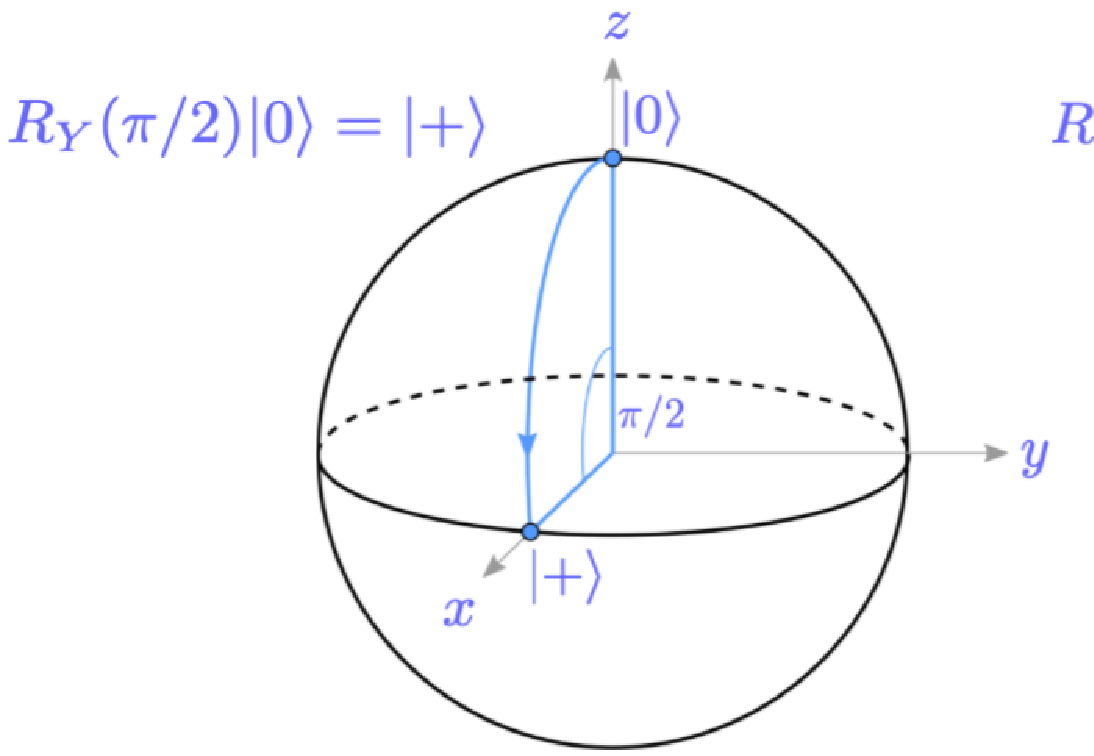
\includegraphics[width=0.7\textwidth]{lesson2/bloch_y_axis.pdf}
    \label{fig: 1}
    \begin{center}
        \caption{Y軸回転}
    \end{center}
\end{figure}
例えばこれがY軸を回転したい場合するとこのY軸はこの場合左右にありますが、まずはinput stateを0にするとこの場合
$\pi/2$の$Y$の回転にすると
\begin{equation}
R_{Y}(\pi / 2)|0\rangle=|+\rangle
\end{equation}
プラスの状態というのはこの角度を$\pi/2$回転するでしょう。で北極の所から赤道まで下がる。するとこれがX軸のてっぺんの所の+になります。まあこれだけじゃなく色んな場所で回転は可能です。
\begin{figure}[H]
    \centering
    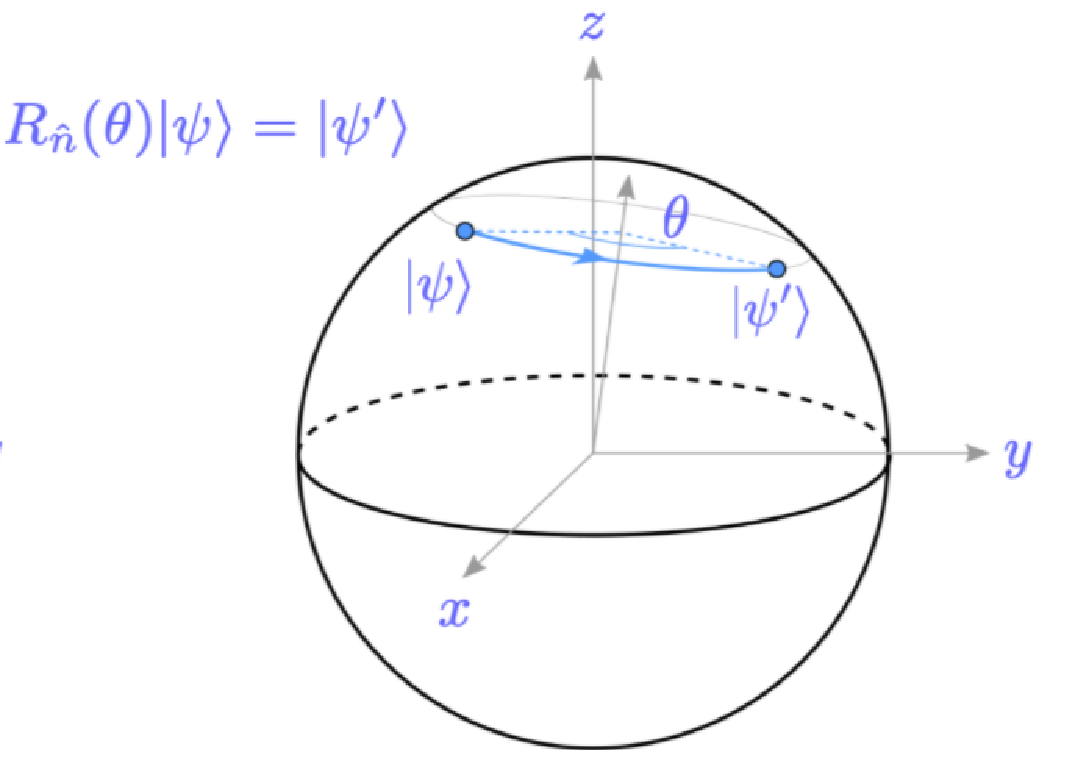
\includegraphics[width=0.7\textwidth]{lesson2/bloch_general_axis.pdf}
    \label{fig: 1}
    \begin{center}
        \caption{任意軸回転}
    \end{center}
\end{figure}
この場合斜めのベクトルを軸としてこの上で回転したいので$\psi$の状態を$\psi^\prime$に回転することがこれがさっきの汎用の所の
\begin{equation}
R_{\hat{n}}(\theta)|\psi\rangle=\left|\psi^{\prime}\right\rangle
\end{equation}
これがユニタリ演算の基礎の数学です。

\section{測定}
測定の目標としてはシステムから情報を読み出す。読み出しが量子のデータから古典のデータになるんですけれども、例えば一番知りたい事はこの量子ビットが0の状態か1の状態かどっちですか?その質問を答えたいです。
\subsection{パウリZ軸測定}
\begin{figure}[H]
    \centering
    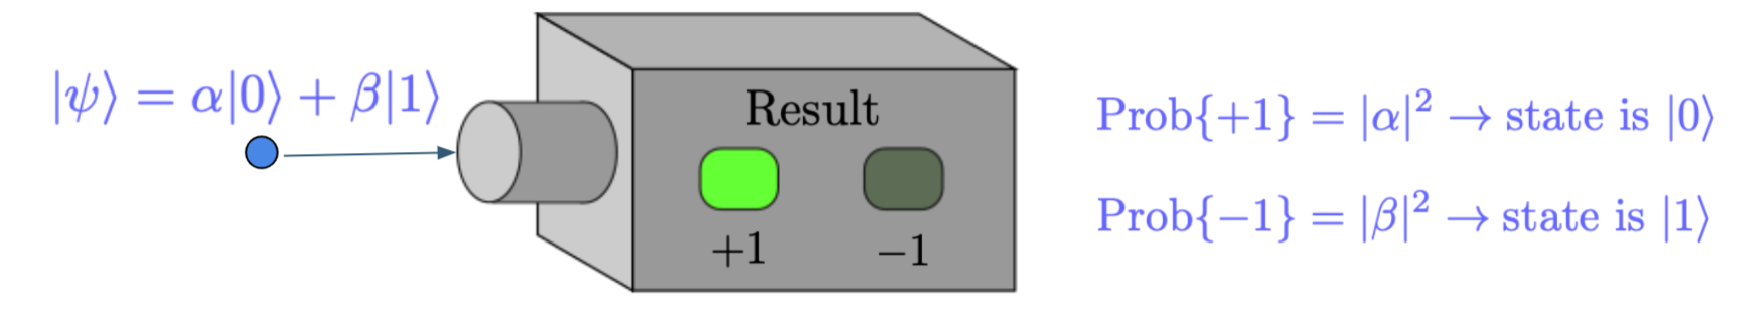
\includegraphics[width=0.7\textwidth]{lesson2/Pauli_z_machine.pdf}
    \label{fig: 1}
    \begin{center}
        \caption{Z軸測定}
    \end{center}
\end{figure}
じゃあ例えばこれが機械になるんですけれどもinputとしては何か知らない量子ビットの状態を入れるんですがこの装置に入れて出てくる結果が$+1$か$-1$が出てきます。

その$+1$か$-1$だったらまあこの場合その最初のインプットの$\psi$のstateが
\begin{equation}
|\psi\rangle=\alpha|0\rangle+\beta|1\rangle
\end{equation}
の状態だったらその$+1$出てくる確率が絶対$|\alpha|^{2}$で$-1$が出てくる確率が絶対$|\beta|^{2}$
そうするとこれが \textbf{Quantum measurement}の基礎です。この場合だったらパウリのZ軸で測定するんですけれどもさっきのブロッホ球の所にはこれがブロッホ球の一番上か下になる事なんですね。これは \textbf{computational basis}と言いますけれどもそれが計算基底ですね。
\subsection{パウリX軸測定}

まあもう一つの測定の仕方があるんですけれども、この状況は0状態が0ですか1ですかじゃなくてこの状態が+ですか-ですかとの質問も問うことが可能でしょう。
すると線形代数を使うと:
\begin{equation}
|0\rangle=\frac{1}{\sqrt{2}}(|+\rangle+|-\rangle) \quad|1\rangle=\frac{1}{\sqrt{2}}(|+\rangle-|-\rangle)
\end{equation}
と表示できます。1の状態だったらマイナスの状態には位相をつけるでしょう。
\begin{figure}[H]
    \centering
    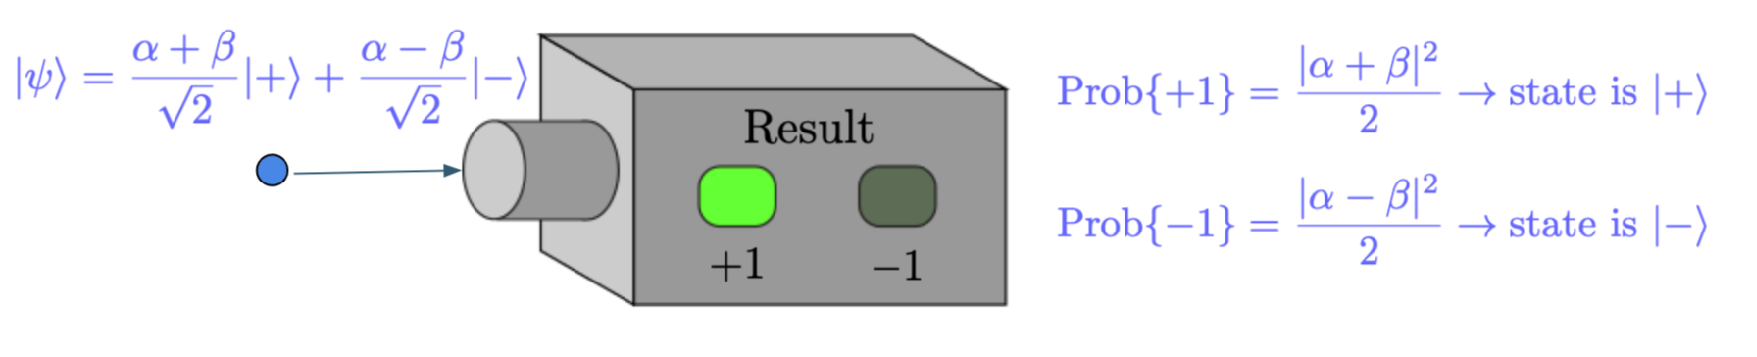
\includegraphics[width=0.7\textwidth]{lesson2/Pauli_x_machine.pdf}
    \label{fig: 1}
    \begin{center}
        \caption{X軸測定}
    \end{center}
\end{figure}
そうするとこの状態を入れると:
\begin{equation}
|\psi\rangle=\frac{\alpha+\beta}{\sqrt{2}}|+\rangle+\frac{\alpha-\beta}{\sqrt{2}}|-\rangle
\end{equation}
そうすると$+1$が出てくる確率が$\alpha +\beta$の絶対値とそれの二乗割る2、-1が出てくる確率が$\alpha-\beta$の絶対値二乗割る2。そうするとこれがが$+$になってくる確立と$-$で出てくる確率はそれも表示できます。
これは\textbf{Pauli X Basis}、\textbf{Figure 1.10}のブロッホ球のところに$+$がX軸のブロッホ球の赤道のところには X軸の一番手前のところと$-$が一番後ろでしょう。そうするとこれがその状態として表示できます。
\subsection{線形代数}
さてこれは基底と言ってるんですけれども$0$, $1$の基底あるいは$+$,$-$の基底と言います。線形代数の授業で学んだと思うんですけれども\textbf{basis set}このbasis setというのは基底setなんですがそれがベクトルどんなベクトルも表示できるベクトルのセットと言える。2次元の紙だったらX軸+Y軸だったらなんでもその紙の上のところになんでも定義できるでしょう。

まあこの場合だったら$\psi$の状態を表示しているんですけどもこれは\textbf{Pauli Z basis} が0の状態と1の状態。この2つはまあ一つの量子ビットで二次元のシステムなんですけれどもその0と1が基底セットになる。
% Insert basis representation pic here.
\begin{figure}[H]
    \centering
    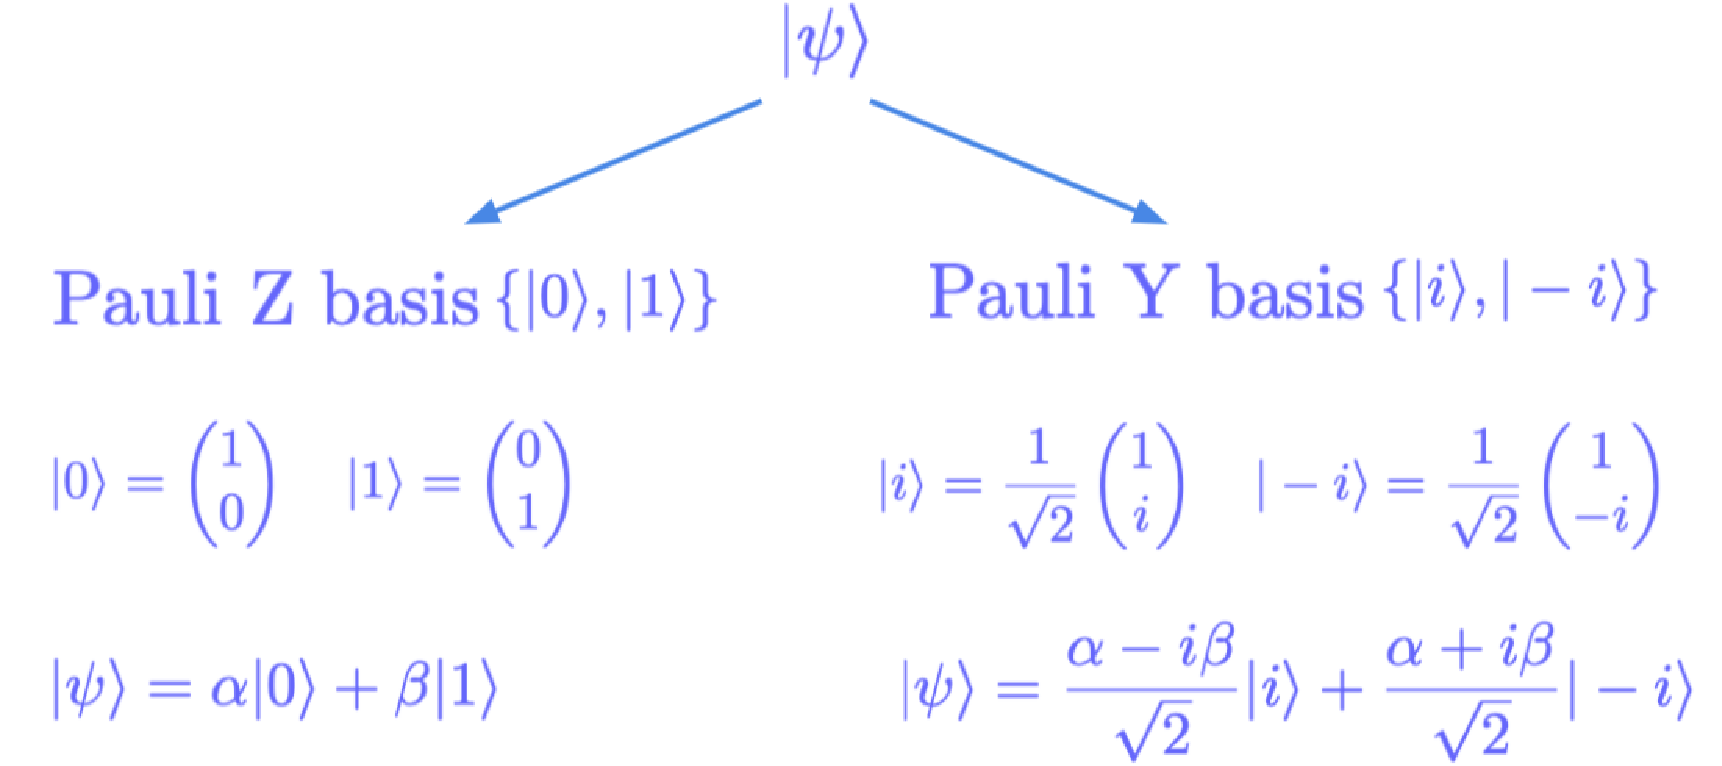
\includegraphics[width=0.7\textwidth]{lesson2/basis_representation.pdf}
    \label{fig: 1}
    \begin{center}
        \caption{基底表示}
    \end{center}
\end{figure}

%0=1, 0のベクトルと1が0, 1のベクトルで\phi=\alpha 0 + \beta %1。これがまあなんで可能な1つの量子ビットの状態を表示できるセット。このセ%ット0と1は十分です。そうするとこれが\textbf{completeなbasis} setです。
%もう一つの書き方があるんですけれども Z basis じゃなくてY %basisにも使えます。
そうするとbasis setがiの状態と-iの状態
$i$と$-i$それがまあブロッホ球のY軸の右と左のところです。
そうすると$\alpha$と$\beta$はこの表示された様な関係になります。じゃあ
$X$のbasisも$Y$のbasisも$Z$のbasisで書くことは可能なんですけれども、
\textbf{computational basis}(計算基底)としてはそれが一番使われているbasisです。

次の概念に行きましょう Inner product 内積です。
今まではケットを使っていたんですがこれがアングルブラケットの脇に書かれている$\psi$ケット。それと同様に\textbf{bra}もあるんですが逆の方向に書きます。アングルブラケットは左側にあるので braの$\psi$とketの$\psi$があるんですが一緒にするとブラケット, bracketになります。これがDiracのnotationです。

例えばこれが$\psi$のbraにすると$\psi$のdaggerをつけられます。
\begin{equation}
\langle\psi|=(|\psi\rangle)^{\dagger}=\left(\begin{array}{l}
\alpha \\
\beta
\end{array}\right)^{\dagger}=\left(\begin{array}{ll}
\alpha^{*} & \beta^{*}
\end{array}\right)
\end{equation}

すると内積もできます。今までは一つ量子ビットが$|\psi\rangle=\alpha|0\rangle+\beta|1\rangle$と言っていたんですが。もう一つの状態を見てみましょう。もう一つの状態が$|\phi\rangle=\gamma|0\rangle+\delta|1\rangle$で表示すると内積がこのように書けます:
\begin{equation}
\langle\phi \mid \psi\rangle=\left(\begin{array}{ll}
\gamma^{*} & \delta^{*}
\end{array}\right)\left(\begin{array}{c}
\alpha \\
\beta
\end{array}\right)=\alpha \gamma^{*}+\beta \delta^{*}
\end{equation}
$\psi$と$\phi$の内積がこの記号で書くと$\alpha\gamma^{*} + \beta\delta^{*}$になる。これが内積の定義です。これがこの状態がが正規化されている場合には$\phi$の自分の内積、$\phi$と$\phi$の内積、$\phi$のbraと$\phi$のketにすると:
\begin{equation}
\langle\psi \mid \psi\rangle=|\alpha|^{2}+|\beta|^{2}=1
\end{equation}
これは正規化の状況です。これがもう一つの概念にすると
\textbf{orthogonal}だったらこれが直行と言いますが、その直行の状態だったらこの$\psi$と$\phi$の内積が$0$に等しい:
\begin{equation}
\langle\phi \mid \psi\rangle=0
\end{equation}
これが定義になります。

\subsection{確率的な測定}
では続きで確率的な測定をすることが
この$\phi=\alpha\ket{0}+\beta\ket{1}$、まあこれが別の基底で測定すると
$\{\ket{b_0}, \ket{b_1}\}$の基底を例にすると:
\begin{equation}
\operatorname{Prob}\{+1\}=\left|\left\langle b_{0} \mid \psi\right\rangle\right|^{2} \quad \operatorname{Prob}\{-1\}=\left|\left\langle b_{1} \mid \psi\right\rangle\right|^{2}
\end{equation}
$+1$の確率がその$b_0$と$\psi$の内積の絶対値の二乗とその$-1$が出てくる確率が$b_1$と$\psi$の内積の絶対値の二乗。
\begin{figure}[H]
    \centering
    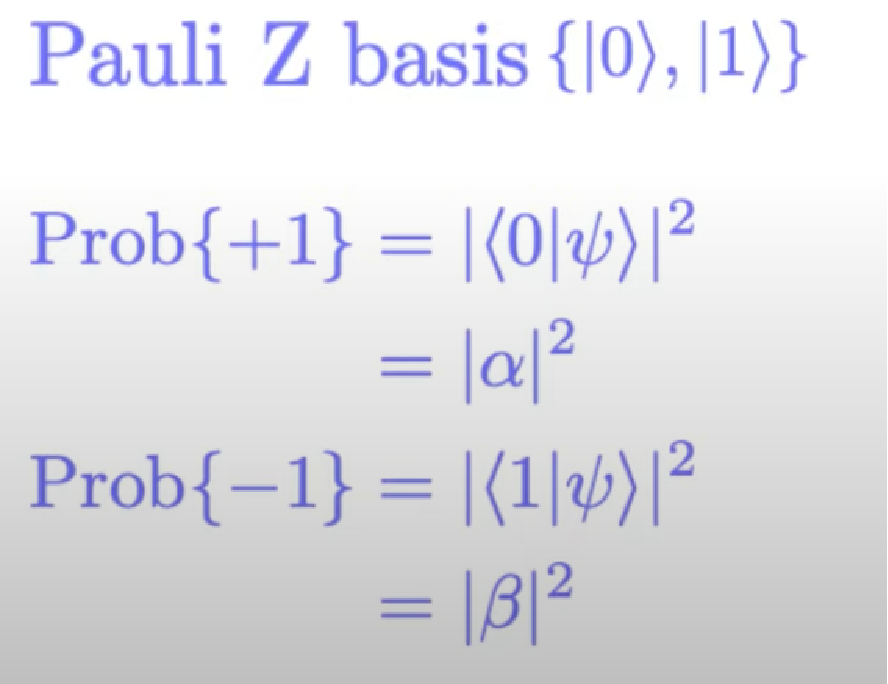
\includegraphics[width=0.5\textwidth]{lesson2/Pauli_z_ex.pdf}
    \label{fig: 1}
    \begin{center}
        \caption{確率:Z軸測定}
    \end{center}
\end{figure}
例えばこれがまあいつも使っているZ軸で計算基底なんですけれども+1の出てくる確率は$0$のベクトルと$\psi$のベクトルの内積でこれを計算すると$\alpha$の絶対値の二乗が出てくる。$-1$の確率が$1$のベクトルなんですけれども$1$のベクトルと$\psi$の内積の絶対値の二乗です。これも$\beta$絶対値の二乗です。これが計算ベクトルで測定してその結果から出てきます。
% Pauli Y example
\begin{figure}[H]
    \centering
    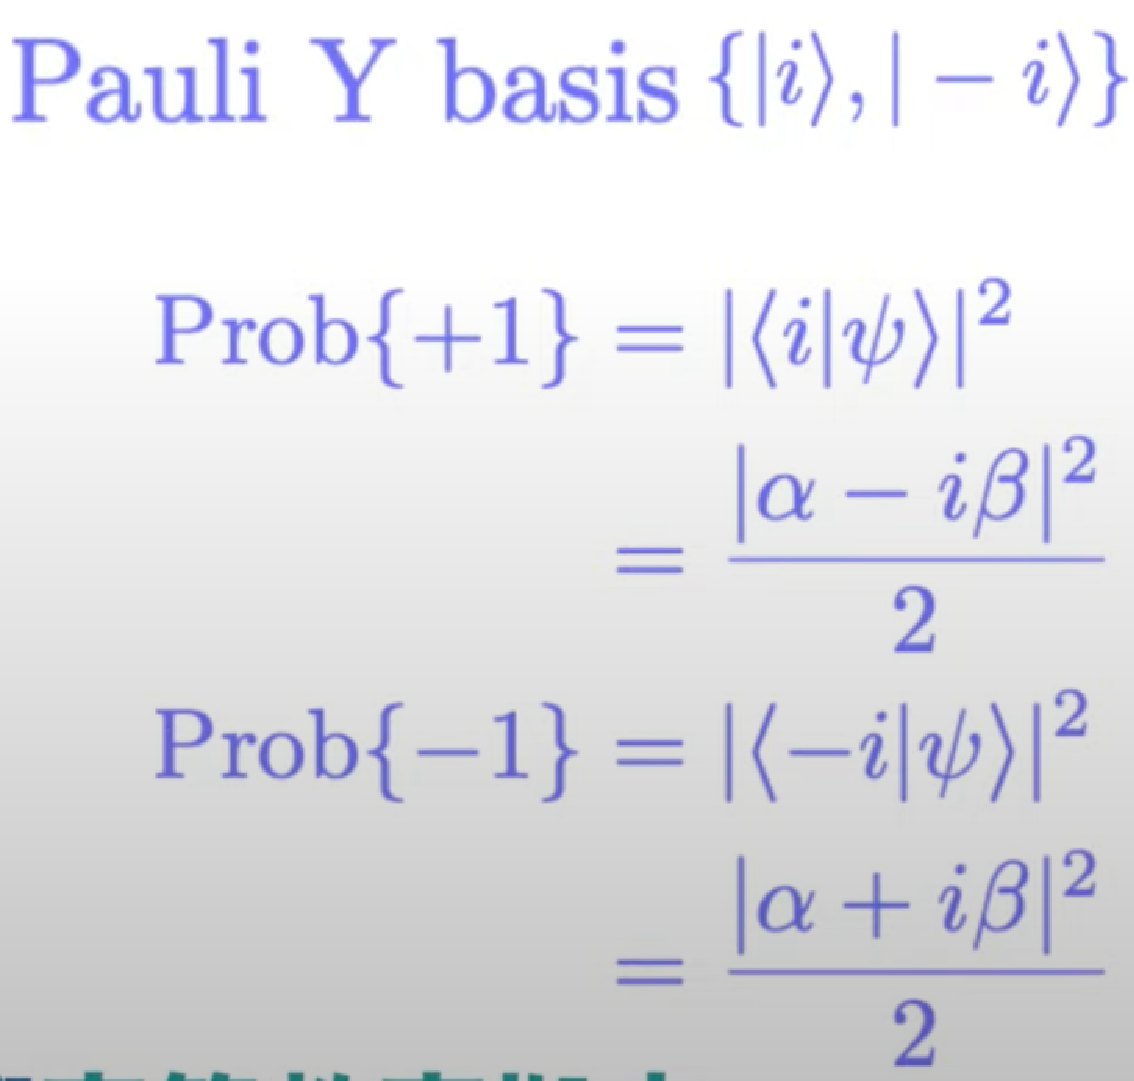
\includegraphics[width=0.5\textwidth]{lesson2/Pauli_y_ex.pdf}
    \label{fig: 1}
    \begin{center}
        \caption{確率:Y軸測定}
    \end{center}
\end{figure}
もう一つの例を挙げると先ほど使っていたYの基底なんですがこのYの基底にすると$i$と$-i$これも同じ風に計算すると$i$と$\psi$の内積を使ってその絶対値をとってそれを二乗にすると出てくるのが$\alpha-i\beta$絶対値の二乗割る2と同様に$-1$もこの表示で出てきます。


\section{確率、期待値、分散}
\subsection{確率}
確率、期待値、分散。Probabilities, expectation, and variance.じゃあちょっと見てみましょう。
先程ステップ3が終わった所なんですけどそれが一つの量子状態を測定したら1回だけの結果が出てきてその状態を破壊して新しい状態が生まれるでしょう。
最後にもっと最初の状態を知りたいなら繰り返さなければいけないと言ってたでしょう。じゃあそれをもうちょっと見てみましょう。
% many copies machine
\begin{figure}[H]
    \centering
    \includegraphics[width=0.5\textwidth]{lesson2/many_copies_machine.pdf}
    \label{fig: 1}
    \begin{center}
        \caption{複数の状態測定}
    \end{center}
\end{figure}
さて、その情報を知りたいなら最初の状態を繰り返していくつかのコピーを作ってそれを連続で測定します。まあそうすると、このように装置が作れるんですが
$\psi$と同じ状態を繰り返し作ってこの機械に入れて出てくることが$-1$, $+1$, $-1$, $+1$の結果が連続で出てくるでしょう。すると$+1$が出てきた数が$N(+1)$と言いますし$-1$が出てきた数が$N(-1)$。これが$\alpha$と$\beta$の情報が計算できるようになります。
\begin{equation}
\begin{aligned}
&\frac{N(+1)}{N(+1)+N(-1)} \approx|\alpha|^{2} \\
&\frac{N(-1)}{N(+1)+N(-1)} \approx|\beta|^{2}
\end{aligned}
\end{equation}

まあこの$N(+1) + N(-1)$はこれが何回このプロセスを繰り返したかを表していると言えるでしょう。それが合計は$\alpha$の絶対値の二乗ぐらいになるでしょう。$N(-1)$を割ると合計が$\beta$の絶対値二乗ぐらいになって-1の出てくる確率になります。

\subsection{期待値}
そうするとこれの期待値はどうなるでしょう。これが基底によります、例えば計算基底、Pauli Z basisの場合の期待値を考えた時Eは確率の授業などで勉強したように:
\begin{equation}
\begin{aligned}
\mathbb{E}[Z] &=\operatorname{Prob}(+1) \cdot(+1)+\operatorname{Prob}(-1) \cdot(-1) \\
&=|\alpha|^{2}-|\beta|^{2}
\end{aligned}
\end{equation}
\textbf{expectation value}(期待値)を例えばこれをDiracの書き方にすると例えばZの基底なのでZをangle bracketの中に入れるとexpectation value(期待値)を示す。

\begin{equation}
\langle Z\rangle=\langle\psi|Z| \psi\rangle
\end{equation}
計算を確認して$\alpha$の絶対値の二乗引く$\beta$の絶対値の二乗になる:
\begin{equation}
\begin{aligned}
\langle Z\rangle &=\left(\begin{array}{ll}
\alpha^{*} & \beta^{*}
\end{array}\right)\left(\begin{array}{cc}
1 & 0 \\
0 & -1
\end{array}\right)\left(\begin{array}{l}
\alpha \\
\beta
\end{array}\right) \\
&=\left(\begin{array}{ll}
\alpha^{*} & \beta^{*}
\end{array}\right)\left(\begin{array}{c}
\alpha \\
-\beta
\end{array}\right) \\
&=|\alpha|^{2}-|\beta|^{2}
\end{aligned}
\end{equation}
これがPauliのZ basis、Z 基底で測定するとこういう結果が出てきます。
\subsection{分散}
もう一つの用語を使うと分散、英語でvarianceと言いますが、出てくる結果が確率的だが最終的には確率が出てきてそのどのぐらいずれている可能性があるかを知りたい場合確率の分布を考えるために分散の概念は必要でしょう。
\begin{equation}
\begin{aligned}
\operatorname{Var}[Z] &=\mathbb{E}\left[Z^{2}\right]-\mathbb{E}[Z]^{2} \\
\mathbb{E}\left[Z^{2}\right] &=\operatorname{Prob}\{+1\} \cdot(+1)^{2}+\operatorname{Prob}\{-1\} \cdot(-1)^{2} \\
&=|\alpha|^{2}+|\beta|^{2}
\end{aligned}
\end{equation}
そうすると\emph{variance}は$Var[Z]$と書いてこれが行列のZの二乗のexpectation value(期待値)引くZの期待値の二乗。もう少し詳しく見ると$\mathbb{E}[Z^2]$の2というのは最初のはbracket(括弧)の中でZの行列の二乗になっており、二つ目では二乗が外なのでZの期待値を測定\emph{してから}二乗している。\textbf{式1.35}が示すように、$\mathbb{E}[Z^2]$は$|\alpha|^2 + |\beta|^2$になります。
%つまりもう少し見るとZの二乗の期待値が+1の確率掛ける-, +1の二乗
% +, -1の確率掛ける-1の二乗なので
% α絶対値の二乗+β絶対値の二乗
% 絶対チヌの事情+データー絶対値の二乗
これは正しく正規化されている場合は$|\alpha|^2 + |\beta|^2 = 1$になるでしょう。

さて最後のこれは時々しか出てきませんがその分散が量子の場合だと\textbf{fluctuation}、 物理学者が使う用語で確率の授業ではvariance(分散)を学んだと思いますが、物理学者はfluctuationという用語を使って\textbf{式1.36}のような書き方もします:
\begin{equation}
\begin{aligned}
(\Delta Z)^{2} & \equiv \operatorname{Var}[Z] \\
&=\left\langle Z^{2}\right\rangle-\langle Z\rangle^{2}
\end{aligned}
\end{equation}

\section{複数の量子ビット}
今まで話たことは例として1量子ビットしか使っていませんでしたがもちろん計算では複数の量子ビットを使いたいですよね。量子通信や量子インターネットに
関しても複数の量子ビットを使いたいでしょう。

まずは複数の古典ビットの場合を復習しましょう。この場合$2^2$の状態は可能ですかね。四つの状態が可能です: $00$, $01$, $10$, $11$。この4つの可能性があります。

量子ビットだったら二つの量子ビットの場合同様です。先程の

$\ket{00}, \ket{01}, \ket{10}, \ket{11}$も同じように出てくるでしょう。この場合これは基底ベクトルだと言えます。そうすると一般的の状態を表示すると、二つの量子ビットの場合このように書きます:
\begin{equation}
|\psi\rangle=\alpha|00\rangle+\beta|01\rangle+\gamma|10\rangle+\delta|11\rangle
\end{equation}
$\alpha$, $\beta$, $\gamma$, $\delta$も正規化が必要です。
$|\alpha|^2 + |\beta|^2$が1つの量子ビットの状態なんですけれども、
これが2量子ビットで4つの状態が可能になるので
これが4つの項を合わせて1になります:
\begin{equation}
|\alpha|^{2}+|\beta|^{2}+|\gamma|^{2}+|\delta|^{2}=1
\end{equation}
$|\gamma|^2$が式から出てくるんですが、測定するとこれが10が出てくる確率になります。4つの確率を合わせて確率全部を計算すると出てくる確率は1なのでこれが正規化と言います。
\begin{equation}
|00\rangle=\left(\begin{array}{l}
1 \\
0 \\
0 \\
0
\end{array}\right),|01\rangle=\left(\begin{array}{l}
0 \\
1 \\
0 \\
0
\end{array}\right),|10\rangle=\left(\begin{array}{l}
0 \\
0 \\
1 \\
0
\end{array}\right),|11\rangle=\left(\begin{array}{l}
0 \\
0 \\
0 \\
1
\end{array}\right)
\end{equation}
そうすると\textbf{式1.39}が4つの基底ベクトル(basis states)になります。
\subsection{ベクトルのテンソル積}

さて\textbf{式1.39}基底はどのように作れるでしょう。
\textbf{Tensor product} テンソルの掛け算で\textbf{式1.40}で表されている記号を使います:
\begin{equation}
|a\rangle \otimes|b\rangle=\left(\begin{array}{l}
a_{1} \\
a_{2}
\end{array}\right) \otimes\left(\begin{array}{l}
b_{1} \\
b_{2}
\end{array}\right) \equiv\left(\begin{array}{l}
a_{1}\left(\begin{array}{l}
b_{1} \\
b_{2}
\end{array}\right) \\
a_{2}\left(\begin{array}{l}
b_{1} \\
b_{2}
\end{array}\right)
\end{array}\right)=\left(\begin{array}{l}
a_{1} b_{1} \\
a_{1} b_{2} \\
a_{2} b_{1} \\
a_{2} b_{2}
\end{array}\right)
\end{equation}
丸の中にばつがある記号です。これが「aのket掛けるbのket掛ける」とも言いますがテンソルの掛け算なので計算の手法が少し違います。テンソルの掛け算と言う場合もありますが、普段は掛け算と省略します。説明のためテンソルを使いたいと思います。

この$
\left(\begin{array}{l}
a_1 \\
a_2
\end{array}\right)$のベクトルと$\left(\begin{array}{l}
b_1 \\
b_2
\end{array}\right)$のベクトルのtensor productを取りたいの\textbf{式1.40}に見えるように解きます。
%で二つ目(後者)のb1 b2のベクトルを
%こっちに置いてそれを掛ける
%前者のベクトルa1 a2と
%a1掛けるb1 b2のベクトル
%下の所でも同じように
%b1 b2のベクトル掛けるそのa2の所で
%前者の所で掛け算になり
%後者のベクトルをそのまま置いて掛けると
%出てくる結果がa1 b1, a1 b2, a2 b1, a2 b2
例として:
\begin{equation}
|0\rangle \otimes|1\rangle=\left(\begin{array}{l}
1 \\
0
\end{array}\right) \otimes\left(\begin{array}{l}
0 \\
1
\end{array}\right)=\left(\begin{array}{l}
0 \\
1 \\
0 \\
0
\end{array}\right)
\end{equation}
$\ket{0}$のベクトルと$\ket{1}$のベクトルをtensor productすると、\textbf{式1.41}で見える通りに解けます。
%この1, 0掛ける0, 1にすると
%まあ1掛けるこの0, 1のベクトル
%この上の半分はそうなり
%下の半分が前者の0掛けるこの0, 1のベクトルで
%これが0, 0になります
もう一つの例として例えば:
\begin{equation}
|1\rangle \otimes|-\rangle=\left(\begin{array}{l}
0 \\
1
\end{array}\right) \otimes \frac{1}{\sqrt{2}}\left(\begin{array}{c}
1 \\
-1
\end{array}\right)=\frac{1}{\sqrt{2}}\left(\begin{array}{c}
0 \\
0 \\
1 \\
-1
\end{array}\right)
\end{equation}
%これが
%1掛ける−の状態
%0, 1のベクトル掛ける√1/2の1, −1のベクトル
%そうするとこの最初の0, 上の0掛ける
%この1, −1のベクトルで上の所は0, 0になるでしょう
%下の所にはこの1掛けるこの1, -1でこれが出てきて
%このconstant(定数)の所には√1/2が出てきます

\subsection{行列のテンソル積}
さてそれがベクトルのtensorの掛け算でしたが、行列でもできます:
\begin{figure}[H]
    \centering
    \includegraphics[width=0.8\textwidth]{lesson2/matrix_tensor.pdf}
    \label{fig: 1}
    \begin{center}
        \caption{行列のテンソル}
    \end{center}
\end{figure}
これは$A$の行列と$B$行列の掛け算なんですが、これが普通のベクトルの行列の掛け算ではなくtensorの掛け算なのでtensorproductとしてはこの丸ばつの記号を使います。
\iffalse
%ちょっと拡大するとAの行列はA11 A12 A21 A22
tensor product

0:06:45.608,0:06:50.229
B11 B12  B21 B22で

0:06:50.230,0:06:56.528
すると後者のBの行列を

0:06:56.529,0:07:00.520
そのままこっちに入れて掛けると

0:07:00.837,0:07:10.273
前者のA11でA12 A21 A22の各所に

0:07:10.274,0:07:12.274
Bの行列を掛ける
\fi
そうして全ての組み合わせが出てきて最初の行列が2掛ける2の行列でしたが
結果としては4掛ける4の行列になります。


\begin{equation}
(A \otimes B)|a\rangle \otimes|b\rangle=A|a\rangle \otimes B|b\rangle
\end{equation}
\textbf{式1.43}も\emph{Dirac notation}ですけれども
この場合だったら大文字の$A$が小文字の$a$の状態に演算してますし、この大文字の$B$と小文字の$b$をすると最初の方には$(A \otimes B)|a\rangle \otimes|b\rangle$は右側に等しいです。
\iffalse
かっこa状態tensor product b の状態=

0:08:08.781,0:08:11.571
Aの行列掛けるaの状態掛ける

0:08:11.571,0:08:17.380
tensor product Bの行列掛けるbの状態です
\fi

さて例として見てみましょう。パウリXの演算子を最初の量子ビットだけに作用させましょう:
\begin{equation}
\begin{aligned}
(X \otimes I)|\psi\rangle &=X \otimes I(\alpha|00\rangle+\beta|01\rangle+\gamma|10\rangle+\delta|11\rangle) \\
&=\alpha|10\rangle+\beta|11\rangle+\gamma|00\rangle+\delta|01\rangle
\end{aligned}
\end{equation}
そうすると$(X \otimes I)$は二つ目の量子ビットには何もしないという事を表示しています。
\iffalse
掛けるΨの状態

0:08:43.340,0:08:48.630
それは= X掛けるI

0:08:48.630,0:08:58.572
tensorの掛け算掛けるα00 + β01 + \gamma10 + δ11

0:08:58.572,0:09:08.086
するとα10 +β11 + \gamma00 + δ01
\fi
まあこの掛け算は細かく説明する必要がないと思いますが自分でやってみると良いと思います。でもその最初のX掛けるIを見てみると:
\begin{equation}
(X \otimes I)=\left(\begin{array}{ll}
0 & 1 \\
1 & 0
\end{array}\right) \otimes\left(\begin{array}{ll}
1 & 0 \\
0 & 1
\end{array}\right)=\left(\begin{array}{llll}
0 & 0 & 1 & 0 \\
0 & 0 & 0 & 1 \\
1 & 0 & 0 & 0 \\
0 & 1 & 0 & 0
\end{array}\right)
\end{equation}
左上の部分は全部0になり、右上の部分はこれが$I$になる。左下も$I$になるんですけども右下の所は全部0になります。じゃあ細かいレベルで見ると後者の$\left(\begin{array}{ll}
1 & 0 \\
0 & 1
\end{array}\right)$の行列がありますがもうちょっと拡大(zoom out)して見ると
この形は前者の$\left(\begin{array}{ll}
0 & 1 \\
1 & 0
\end{array}\right)$ の行列と似ているでしょう。この様に掛け算はします。

\chapter[純粋状態と混合状態]
{純粋状態と混合状態}

\section{雑音の世界}
\subsection{理想と現実}
まあ今までの喋ってた状態についてはその量子状態が完璧だと考えているんですけれど、それは\textbf{ノイズ}(雑音)をかけられてないものなんですね。実世界にはそれ(ノイズのない状態) を作ることは不可能でしょう。応用できません。
\subsection{状態制作}
例えば、友達のラボラトリーに行ったらその友達には「この$\psi$のステートを作ってちょうだい」とお願いしたら、友達は何を作ってくれるでしょう?
その友達が作ってくれる状態が、$\psi^\prime$(プサイダッシュ)なんですが、$\psi$ではないことが多いですね。

だが、それが完璧に何をつくってくれるか、まぁそれでも使えるんですけれども、実は確率的な状態になるでしょう。
% state preparation
\begin{figure}[H]
    \centering
    \includegraphics[width=1.0\textwidth]{lesson3/state_creation.pdf}
    \label{fig: 1}
    \begin{center}
        \caption{状態作りのノイズ}
    \end{center}
\end{figure}
例えば、 $p1$の状態で$\psi_1$の状態作ることは可能かもしれないし$p2$の確率で$\psi_2$の状態をつくったら、まあこういう分布にはなるんですがそのstate が。しょうがないんですね。これが世の中のルール、現実のことです。
それと、state、状態を作ることだけじゃなくて、stateの
\subsection{演算}
演算とかも同じなんですよね、情報処理の。その情報処理は、例えば「この$U$のユニタリー演算をかけてちょうだい」と友達に言うかもしれないんですが、出てくる結果が
$U\psi$ではない可能性は結構高い。

もうちょっと喋るとかけている$U^\prime$ (Uダッシュ)の状態が$U$ではないですね。
数学的には書くとこれも\textbf{コヒーレントのエラー}だけじゃなくて
それも\textbf{インコヒーレントのエラー}の可能性があるんですけれども、そのインコヒーレントという場合だったらこれがユニタリー演算ではないことになるかもしれない:
% processing of information
\begin{figure}[H]
    \centering
    \includegraphics[width=1.0\textwidth]{lesson3/information_processisng.pdf}
    \label{fig: 1}
    \begin{center}
        \caption{演算のノイズ}
    \end{center}
\end{figure}
じゃあ、どうしましょう?
\subsection{量子通信}
Quantum Communications(量子通信)は同じですよね。
例えば、光ファイバーにstateを通すとき、まぁ最初の$\psi$のstateを送るんですが
相手に届くstateが$\psi$ではない。
% quantum communications
\begin{figure}[H]
    \centering
    \includegraphics[width=1.0\textwidth]{lesson3/quantum_communications.pdf}
    \label{fig: 1}
    \begin{center}
        \caption{量子通信のノイズ}
    \end{center}
\end{figure}

まあそのコヒーレントエラー、つまりその先の例としてはビットフリッピ(bit flip)の$X$のユニタリー演算とか。あるいは、インコヒーレントエラーとか。あるいは光ファイバー通す光子がなくなる可能性があるでしょう。そのなくなることを\textbf{「減衰」}と言いますね。そのファイバーのattenuation(減衰)です。
\subsection{まとめ}
これが実のことなんですけれども、どうやって数学的にこれが書けるでしょう
どうやって表示して、どうやって対応できるでしょう?

\section{外積}
今までは内積を見たんですけれども、それが2つの量子状態の掛け算の一つなんですけれども。そのことは、こういうふうに書けますでしょう:
\begin{equation}
\langle a \mid b\rangle=\left(\begin{array}{ll}
a_{0}^{*} & a_{1}^{*}
\end{array}\right)\left(\begin{array}{l}
b_{0} \\
b_{1}
\end{array}\right)=a_{0}^{*} b_{0}+a_{1}^{*} b_{1}
\end{equation}
\iffalse
a のブラとbのケット(*ブラケット記法)が、

0:00:22.440,0:00:30.320
aの横のベクトルとbの縦のベクトルにすると、これがまあ

0:00:31.380,0:00:35.890
複素共役にされている

0:00:35.890,0:00:47.089
aのベクトルとbのベクトルにすると、
こういうふうになるでしょう。
\fi
\textbf{式3.1}はscalar(定数)にはなるのですが、これがComplex(複素)になるでしょう。この$a$と$b$ の順番を入れ替えると、内積が
外積になるんです。inner product(内積)がouter product(外積)になるんです。するとこういうふうに書くでしょう:
\begin{equation}
|b\rangle\langle a|=\left(\begin{array}{l}
b_{0} \\
b_{1}
\end{array}\right)\left(\begin{array}{ll}
a_{0}^{*} & a_{1}^{*}
\end{array}\right)=\left(\begin{array}{ll}
a_{0}^{*} b_{0} & a_{1}^{*} b_{0} \\
a_{0}^{*} b_{1} & a_{1}^{*} b_{1}
\end{array}\right)
\end{equation}
こうするとスカラーじゃなくて、これが行列にはなるんです。これは複素数の行列になるんです。
さて、これは何に使えるでしょう?なぜ?
外積は役に立つものです:
\begin{enumerate}
    \item 1:測定の結果に表示できます。さっきのステップで測定のことを話してたんですが、これは測定の結果、それが表示できることです
    \item 2:量子状態の新しい表示の仕方になります。それがこのレッスンの一つの大きなポイントになる。
\end{enumerate}

\subsection{測定の結果表示}
さて、$\bra{0}\ket{0}$のオペレーター、この演算と、$\bra{1}\ket{1}$のオペレーター、これの演算が、$\psi$の状態にはどう影響するのか?どう作用するのか?

じゃあ書きますと:
\begin{equation}
\begin{aligned}
|0\rangle\langle 0 \mid \psi\rangle &=|0\rangle\langle 0|(\alpha|0\rangle+\beta|1\rangle)\\
&=\alpha|0\rangle\langle 0 \mid 0\rangle+\beta|0\rangle\langle 0 \mid 1\rangle \\
&=\alpha|0\rangle
\end{aligned}
\end{equation}

$|0\rangle\langle 0 \mid \psi\rangle$これは外積かけるその$\psi$の状態なんですが、掛け算のルールによるとこの$\bra{0}$と$\psi$が\textbf{式3.3}のように内積になることも可能です。

すると、
\iffalse
この0ケット0ブラ

0:03:20.730,0:03:27.290
× $\alpha$0ケット + $\beta$1ケットが

0:03:27.290,0:03:34.710
$\alpha$ × 0 × 0ケット × 0 ブラ

0:03:34.710,0:03:42.810
× 0ケット + $\beta$ × 001にすると
\fi
$\braket{0|0}$
ゼロとゼロの内積これが正規化されているベクトルの実行の内積なんですが、その実行の内積にすると、これの結果は1です。じゃあ、それが1なりますから、$\alpha\ket{0}$を残すことになります。それから、右側にある$\braket{0|1}$、これが直交のベクトルなんですが$0$のベクトルと$1$のベクトル。直交のベクトルの内積は$1$じゃなくて、これは$0$になるんですね。そうすると、このterm(項)は消えます。
そうすると、残りの結果が$\alpha\ket{0}$になるんです。


これはこの$\ket{0}\bra{0}$のオペレーターが$\ket{0}$に\textbf{プロジェクション}することなんですが、それが射影することです。このオペレーターは$\ket{0}$の状態には射影することです。これはpauli Z basis(パウリ行列の固有状態のZ basis)の測定の結果によると、これが$+1$の結果の状態になるんです。これが
この前(レッソン2.3)の測定のことを話していたところでは、測定の結果次第では、状況が破壊することになるんですけれども。それの残りが何かの基底のベクトルになるでしょう。まあ、そういう場合には、数学的にはこういうプロジェクションのオペレーターを使うんですね。

それと、1の場合には、 $\ket{1}\bra{1}\psi$だったら、
同じルールを使うと、残りのことろは、$\beta\ket{1}$になります:
\begin{equation}
\begin{aligned}
|1\rangle\langle 1 \mid \psi\rangle &=|1\rangle\langle 1|(\alpha|0\rangle+\beta|1\rangle)\\
&=\alpha|1\rangle\langle 1 \mid 0\rangle+\beta|1\rangle\langle 1 \mid 1\rangle \\
&=\beta|1\rangle
\end{aligned}
\end{equation}
これは、$\ket{1}\bra{1}$のオペーレーターが$\ket{1}$にはプロジェクションする。射影することです。
これはPauli Z matrix、Pauli Z basis、パウリZ規定の測定の-1の結果になればいいです。

さて、\textit{他の基底で測定するとどうなるでしょう}?
さっきの話は、Pauli Z basis、つまり計算の規定なんですけれども、\textbf{Pauli X basis}、これはプラスとマイナスのbasisにもなるんですが。
すると$\ket{+}\bra{+}$の外積かける$\psi$が、そのアウトプット、その結果が測定の結果が$+1$の場合。$-1$の場合も\textbf{式1.5}で表されています:
\begin{equation}
\begin{aligned}
&|+\rangle\langle+\mid \psi\rangle=\frac{\alpha+\beta}{\sqrt{2}}|+\rangle \\
&|-\rangle\langle-\mid \psi\rangle=\frac{\alpha-\beta}{\sqrt{2}}|-\rangle
\end{aligned}
\end{equation}
これは、測定の結果が +1 の場合なんですが
\iffalse
結果が -1 の場合だったら、
$\alpha$ + 1 じゃなくて(* 訂正 "$\alpha$ + $\beta$")、$\alpha$ - $\beta$(正しくは) 
\fi
$\alpha+\beta$ じゃなくて、$\frac{\alpha-\beta}{\sqrt{2}}\ket{-}$の状態です。すると、これが -1の測定の結果にすると、これがマイナスのstateのプロジェクションにしました。

\textbf{Pauli Y basis}で測定すると:
\begin{equation}
\begin{gathered}
|i\rangle\langle i \mid \psi\rangle=\frac{\alpha-i \beta}{\sqrt{2}}|i\rangle \\
|-i\rangle\langle-i \mid \psi\rangle=\frac{\alpha+i \beta}{\sqrt{2}}|-i\rangle
\end{gathered}
\end{equation}
同じようには、$\ket{i}\bra{i}\psi$ の場合だったら$+1$の結果の場合。
$-1$の結果の場合だったら\textbf{式3.6}のように表します。


\begin{equation}
\Pi_{\pm}^{B}=\left|b_{\pm}\right\rangle\left\langle b_{\pm}\right|
\end{equation}
\textbf{式1.7}はもう一つ書けることなんですけれども、これはよく使うことがあると思います。例えば測定のbasisが大文字のΠ(パイ)の字を使えますし
\textbf{式1.7}の右側は$b$の外積にします。すると、この$\Pi$の上付き、これが基底です。これは大文字のBの基底で測定すると表示してます。
下付きのプラスマイナス、これがアウトカム。これが結果と表示します。そうすると、\textbf{式1.7}の右側は$\ket{b_+}\bra{b_+}$結果と$\ket{b_-}\bra{b_-}$の結果と表示することができます。
例とすると:
\begin{figure}[H]
    \centering
    \includegraphics[width=1.0\textwidth]{lesson3/outer_product_examples.png}
    \label{fig: 1}
    \begin{center}
        \caption{$\Pi$表現の例}
    \end{center}
\end{figure}
\iffalse
Pauli Xの規定にすると、Π(パイ)の

0:08:47.420,0:08:53.779
X乗と、subプラスのところ、それが

0:08:53.779,0:09:01.220
プラスプラスの外積。
Π(パイ)をXとマイナスでは、こういうふうに書きますと、

0:09:01.220,0:09:09.300
これがマイナスマイナスの外積になります。
PauliのY basisだったら、こういうふうには書いてて、まぁこれも同様

0:09:09.300,0:09:15.840
に ii の外積と -i -iの外積になるんです。

0:09:15.840,0:09:24.819
Z basisだったら、さっきの例によると、00の外積と、11の外積になる。
\fi
\subsection{量子状態の表示}
0:09:24.819,0:09:32.920
さて、今まで話してきたことは、量子状態がケット(ket)のことを話ししていたのですが定義にすると、0のケットはこの縦のベクトル 。この$\left(\begin{array}{l}
1 \\
0
\end{array}\right)$のベクトル。

0:09:40.180,0:09:46.930
1の状態は縦のベクトルの$\left(\begin{array}{l}
0 \\
1
\end{array}\right)$。

0:09:46.930,0:09:55.830
1キュービットの状態を表示すると、
この$\psi$の変数が、この$\ket{\psi} = \left(\begin{array}{l}
\alpha \\
\beta
\end{array}\right)$の縦のベクトルなんですがこれはケットとベクトルなんですが、これも量子状態も外積に表示できるということです。

例えば、0の状態だったら$\ket{0}$と$\bra{0}$の外積を使って、
行列が$\ket{0}\bra{0}=\left(\begin{array}{ll}
1 & 0 \\
0 & 0
\end{array}\right)$ になる。
1の状態だったら、それの外積は:
\begin{equation}
    \ket{1}\bra{1}=\left(\begin{array}{ll}
0 & 0 \\
0 & 1
\end{array}\right) 
\end{equation}
になる。
もうちょっと汎用なステートにすると、この$\psi$状態にすると:
\begin{equation}
    \ket{\psi}\bra{\psi}=\left(\begin{array}{ll}
|\alpha|^2 & \alpha\beta^{\star} \\
\alpha^{\star}\beta & |\beta|^2
\end{array}\right) 
\end{equation}
\iffalse
$\psi$と$\psi$の外積にすると、$\alpha$の絶対値の自乗、

0:10:38.180,0:10:43.310
$\alpha$$\beta$* 、$\alpha$*$\beta$と

0:10:43.310,0:10:56.150
$\beta$の絶対値の自乗になることです。
\fi
多分、よく見ると、この$|\alpha|^2$と、$|\beta|^2$を見たことがあるでしょう?それの関連は後でもう少し説明します。


\section{密度行列}
今までは、Lesson 2のところには、
量子状態がkets (ケット)で表示してたんですけれども、ketsもベクトルなんですね。

例えば、そのインプットの状態は、$\psi$のketsで書きますし、それも

実の世界では、それがノイズをかけられているチャネルには、転送しますけれども出てくる結果は、$\psi$の状態ではないかもしれないんですけれども、
ここの状態にはなる、確率的に:
% noisy channel pic
\begin{figure}[H]
    \centering
    \includegraphics[width=1.0\textwidth]{lesson3/noisy_channel.pdf}
    \label{fig: 1}
    \begin{center}
        \caption{noisy channel}
    \end{center}
\end{figure}
結果としてです。例えば、$\psi_1$の出てくる確率は$p_1$で$\psi_2$が出てくる確率は$p_2$とか、
$\psi_n$の出てくる確率は$p_n$とか。
これは実世界の結果なんですけれども、これも表示できるようにしたい。
\textit{どうやってそれが表現、表示できるんでしょう}?

重ね合わせについては、普通の重ね合わせは今までは結構しゃべってるんですが、こういうstateが重ね合わせの表示の仕方にも、それを使って出来るんでしょうか?いや、できないんですね。じゃあ、なぜかちょっと見てみましょう。
その重ね合わせは、波の重ね合わせと一緒なんですけれども、その状態が完璧になっているんですね。これが、その完璧の状態は、その重ね合わせには、$0$になる確率と$1$になる確率は別になっているかもしれないんですけれど、あるいはそれは決まってないかもしれないんですが、それがstateについての知識を分かっているのと、分かってないのとは違う。

じゃあ、どうやって証明できるでしょう?どうやって表示できるのでしょう?
確率的な結果が書けるようにならないと、ノイズの影響とかではそれが計算できないから、それがやりたい。すると、今までのこのレッスンで喋っていた外積を使う。

さて、するとさっきの$p_1$、$p_2$、$p$なんとかなんとか、$p_n$になると、
$\psi_1$、$\psi_2$、$\psi$なんとか・・・、$\psi_n$にすると、それがこういうふうに書ける表現になる:
\begin{equation}
p_{1}\left|\psi_{1}\right\rangle\left\langle\psi_{1}\left|+p_{2}\right| \psi_{2}\right\rangle\left\langle\psi_{2}\left|+\ldots+p_{n}\right| \psi_{n}\right\rangle\left\langle\psi_{n}\right|
\end{equation}
\iffalse
0:02:46.610,0:02:50.960
p1 × $\psi$1の外積

0:02:50.960,0:02:59.450
+ p2 × $\psi$2の外積
+ p3 × $\psi$3の外積

0:02:59.450,0:03:08.380
続いて、+ pn × $\psi$nの外積
のようになること。
\fi
これが、一緒なんですが、この$p_1\psi_1$、$p_2\psi_2$、$p_n\psi_n$。こういうふうにしか書けない状態だったら、これが\textbf{mixed state} (混合状態)と言います。このmixed stateはそのエラー等、確率的なこと等、そういうふうに入っているということです。こういうふう表現することは、これはmixed state (混合状態)です。

例を見てみましょう:
% flip channel
\begin{figure}[H]
    \centering
    \includegraphics[width=1.0\textwidth]{lesson3/noisy_channel_bit_flip.pdf}
    \label{fig: 1}
    \begin{center}
        \caption{Noisy flip channel}
    \end{center}
\end{figure}

これはflip channelと言いますけれども、
これは古典のerror correction(エラー訂正)とかInformation theoryとか、情報理論については、これは一生の概念なんですけれども、インプットの状態が$\psi$になってまあ、noisyのchannelを通して出てくる確率は、エラーの場合の確率が、$p$の確率だったら、エラーにならない確率は$1-p$ になるでしょう。じゃあ、最初の状態が、その$\psi$の状態は、それがインプットなんですが、それがアウトプットにもしたいんですけれどもそれの確率は$1-p$。エラーになる場合には、それが$p$の確率でそのアウトプットの結果は $X\ket{\psi}$の状態です。

アウトプットには、こういうふうに密度行列を
使って、こういうふうに表現します:
\begin{equation}
\rho=(1-p)|\psi\rangle\langle\psi|+p X| \psi\rangle\langle\psi| X
\end{equation}
普通には、この密度行列の書き方にすると、変数としては、$\rho$(ロー)。
これが 、p に近い記号なんですけれども、これがギリシャ記号の$\rho$(ロー)なんですけれども。この$\rho$が\textbf{density matrix}、密度行列には使う場合が多いです。

じゃあ、\textbf{式1.11}に二つのterm(項)があるでしょう。このtermがエラーがないtermと、このtermがエラーが起こったtermですね。じゃあ、確率的には正しい状態が出てきた確率は、$1-p$で$(1-p)\ket{\psi}\bra{\psi}$の外積です。

$p$のエラーになった確率が、それが出てくる
のは\textbf{式1.11}の二項目です。
二つ目の$X$は、adjoint (随伴)しなければならないんですけれども。つまり、それは随伴行列しなければならないんですけれども、Xはself adjoint(自己随伴行列)なのでそのまま
$X$を使うことができます。

例えば、
$\ket{\psi}=0$のインプットだったら:
\begin{equation}
\rho=(1-p)|0\rangle\langle 0|+p| 1\rangle\langle 1|=\left(\begin{array}{cc}
1-p & 0 \\
0 & p
\end{array}\right)
\end{equation}
\iffalse
$\rho$(ロー)が

0:06:24.220,0:06:31.350
1- p の 0 の外積 + pの1の外積
\fi
それが$X\ket{0}$ の場合、これがbit-flip(ビットフリップ)のエラーなんですけれども、0が1になるでしょう。そうすると、計算すると、\textbf{式1 1.12}の密度行列になることです:

インプットの状態は、$\ket{\psi}=1$の状態だったら:
\begin{equation}
\rho=(1-p)|1\rangle\langle 1|+p| 0\rangle\langle 0|=\left(\begin{array}{cc}
p & 0 \\
0 & 1-p
\end{array}\right)
\end{equation}
になることです。

もうちょっと汎用的にすると、これが密度行列の事なんですけども、
これが量子状態の一番一般的な表現の仕方です:
\begin{equation}
\rho=\sum_{i} p_{i}\left|\psi_{i}\right\rangle\left\langle\psi_{i}\right|
\end{equation}

さっきのところで、ビットフリップの例もあったし、複数の出て来る可能性のことをちょっとだけ喋ってたんですけれども、もうちょっと汎用的に書くと、その$\rho$の密度行列は、\textbf{式1.14}のふうに書きます。
\iffalse
これが、sumになって、これが i のいくつかの後方のstageにあるんですが、それが 

0:07:55.629,0:07:58.520
p sub i ×

0:07:58.520,0:08:03.879
$\psi$iの外積ということになる。
\fi

これは何に使えるでしょう?
まずは、もちろん、それが今までの喋ったところは\textbf{純粋な状態}なんです。されど、pure state (純粋状態) だったら、それがこの$\rho$の表現にすると、$p_i$ はすべては0なんですが、一つだけの候補が1になっている。まあ、それがpure state (純粋状態) なんですよね。
そうすると、混合状態のmixed stateにはユニタリー演算はもうかけられている
かもしれないし、ユニタリーじゃないノイズもかけられているかもしれないし、
それだったら、この$p_i$は異なっていて、$p_i$ は1と0だけじゃなくて、いくつかの確率にはなるかもしれない。
\subsection{正規化}
レッスン2の喋ったことで、一番最初のところだったんですけれども、純粋状態は正規化しなければならない。じゃあ、それをちょっと見てみましょう。
$\ket{\psi}=\alpha\ket{0}+\beta\ket{1}$だったら、$|\alpha|^2+|\beta|^2=1$
これがその正規化状況ですね。そうすると、密度行列にはどういうふうにはなるんですかね?これは、もう一つの線形代数の概念も必要なんですけれども、これが\textbf{trace} (跡) のこと。
\begin{equation}
\operatorname{Tr}\{A\}=\sum_{i} A_{i i}
\end{equation}
\iffalse
そのtraceはdiagonal(対角)、数学的にはこういうふうに表現ができますけれども、なぜということとか、この大文字の t と小文字の r のオペレーターがこれがtraceと言いますし
\fi
Aが四角の行列をしなければならないんでするとdiagonal(対角)にある数字を足し算すると、これがtraceになる。
例えば、この 3 × 3の行列だったら:
\begin{equation}
\begin{gathered}
A=\left(\begin{array}{ccc}
A_{11} & A_{12} & A_{13} \\
A_{21} & A_{22} & A_{23} \\
A_{31} & A_{32} & A_{33}
\end{array}\right) \\
\operatorname{Tr}\{A\}=A_{11}+A_{22}+A_{33}
\end{gathered}
\end{equation}

そのNormalizationの状態、これが正規化の条件がそういうtrace使うと、そのtraceが1になるべき。例えば純粋のstateだったら:
\begin{equation}
|\psi\rangle\langle\psi|=\left(\begin{array}{l}
\alpha \\
\beta
\end{array}\right)\left(\begin{array}{ll}
\alpha^{*} & \beta^{*}
\end{array}\right)=\left(\begin{array}{ll}
|\alpha|^{2} & \alpha \beta^{*} \\
\alpha^{*} \beta & |\beta|^{2}
\end{array}\right)
\end{equation}
この$\alpha$、$\beta$の縦のベクトルと$\alpha^{\star}$、$\beta^{\star}$の横のベクトルにすると、さっきの計算した通りでdiagonal(対角)のところには、$|\alpha|^2$と$|\beta|^2$、それを合わせると:
\begin{equation}
\operatorname{Tr}\{|\psi\rangle\langle\psi|\}=|\alpha|^{2}+|\beta|^{2}=1
\end{equation}
それが先の言っていたところで、その1キュービットは、こういうふうに
すると、確率的には、何でもの$\alpha$と$\beta$振幅なんですけれども、これにすると、何かを測定すると、結果が出てくるでしょう。その結果が出てくる場合には、1になる。
\subsection{ブロッホ球表示}
さて、混合の状態も、ブロッホ球(bloch sphere)も表示できますけれども、ちょっとだけ複雑です。
さっきのpure state (純粋状態)とは違うんですね。$\psi$は純粋な状態だったら、それが球面、ブロッホ球(bloch sphere)の外側にはあるんです:
% pure state bloch
\begin{figure}[H]
    \centering
    \includegraphics[width=0.5\textwidth]{lesson3/bloch_pure_state.pdf}
    \label{fig: 1}
    \begin{center}
        \caption{ブロッホ球純:純粋状態}
    \end{center}
\end{figure}
mixedの場合には、混合の状態だったら、そのベクトルの長さが、
1 じゃなくて、1より低くて、段々これがブロッホ球の中に行くことになります:
% mixed state bloch 
\begin{figure}[H]
    \centering
    \includegraphics[width=0.5\textwidth]{lesson3/bloch_mixed_state.pdf}
    \label{fig: 1}
    \begin{center}
        \caption{ブロッホ球:混合状態}
    \end{center}
\end{figure}
そうすると、最も極端の例にすると、\textbf{maximally mixed state}と言い
ますが、それが絶対何もわかんない、それが完璧なmixed stateに何も情報が知られていないことなんですけれども、それが
ブロッホ球のど真ん中の点になるのです。
% maximally mixed state bloch
\begin{figure}[H]
    \centering
    \includegraphics[width=0.5\textwidth]{lesson3/bloch_maximally_mixed_state.pdf}
    \label{fig: 1}
    \begin{center}
        \caption{ブロッホ球:最大混合状態}
    \end{center}
\end{figure}

%%%%%%%%%%%%%%%%%%%%%%%%%%%%%%%%%%%%%%
\section{純粋状態と混合状態}
一つのキュービットを考えましょう。これが、一つの例にすると重ね合わせは半分半分0と1なんですが、
それはこういうふうには書くでしょう:
\begin{equation}
|\psi\rangle=\frac{1}{\sqrt{2}}|0\rangle+\frac{1}{\sqrt{2}}|1\rangle
\end{equation}
\textbf{maximally mixed state} という状態なんですが、それが混合状態。それが何にもわからないんですが
ノイズは完璧にかけられている状況なのです。それの密度行列が、
$\rho = \ket{0}\bra{0}$の50\%と$\ket{1}\bra{1}$の50\%を表現できます。
重ね合わせ状態と混合状態を、Pauli Z basisの基底で測定しましょう:
\begin{figure}[H]
    \centering
    \includegraphics[width=1.0\textwidth]{lesson3/pauli_z_measurement.pdf}
    \label{fig: 1}
    \begin{center}
        \caption{Pauli Z 測定}
    \end{center}
\end{figure}
これは、計算基底と言うといいますが。すると、$+1$の確率と$-1$に出てくる確率が両方には、これが50\%の$\ket{0}$になる場合と、50\%の$\ket{1}$になる場合。Mixed stateだったら、混合状態だったら、測定すると、確率の$\ket{0}$になっている状況の確率が50\%で、$\ket{1}$になっている状態の確率、これも50\%なんですね。

じゃあ、これは同じ状態ですか?何が違うでしょう?ちょっと見てみましょう。

X basisにすると、もしかして同じか、もしかして違うんですね。見てみましょう:
\begin{figure}[H]
    \centering
    \includegraphics[width=1.0\textwidth]{lesson3/Pauli_X_measurement.pdf}
    \label{fig: 1}
    \begin{center}
        \caption{Pauli X 測定}
    \end{center}
\end{figure}

重ね合わせ状態はプラスの状態なんですが、その$\ket{+}$の状態はそれがX軸のブロッホ球の一つのてっぺんのところでしょう。だが、混合状態だったら、これがプラスの状態じゃなくて、50\%のプラスプラスの状態と、50\%のマイナスマイナスの状態。これの証明は、面白い課題にはなるかもしれません。

これを射影させることを測定してみると、$+1$の出てくる確率は
その半分半分の重ね合わせの確率が $+1$ が出てくるstateが、
それの100\%の確率です。$-1$の結果が出てくる確率はゼロです。だが、
mixed stateの場合だったら、そのプラスのstateの出てくる確率が50\%と、マイナスのstateが出てくる確率も50\%です。\textit{これは、mixed stateと重ね合わせの違いが証明できます。}
そうすると、結構使い方と、使えるところはそれの結果は結構異なる場合もありますから、是非それを注意していただきたいと思います。
\subsection{まとめ}


\begin{figure}[H]
    \centering
    \includegraphics[width=1.0\textwidth]{lesson3/summary_table.pdf}
    \label{fig: 1}
    \begin{center}
        \caption{Pauli Z 測定}
    \end{center}
\end{figure}

サマライズすると、pure stateとmixed state、純粋のステートと混合のステート
比較してみると、Notation として、記号は何を使うのか?
\begin{enumerate}
    \item $\psi$をステートベクトルに使うんですが、mixed stateだったら、$\rho$の記号を使うでしょう。 これが密度行列になるでしょう。
    \item Pure stateだったら、ベクトルと行列の両方が可能なんですけども、mixed stateの状態だったら、密度行列だけ使えるんです。
    \item 純粋のステートだったら、正規化の条件が内積の自乗は、1に等しく なければならないんですけれども、それは自分の自己内積。密度行列だったら、その行列のtrace (跡) を1にしなければならない。
    \item どのぐらい知られているのか(分かっているのか)?純粋の状態だったら、重ね合わせになっているかもしれないんですけれども、それが重ね合わせです、とはっきり分かっているので、これがperfect (完全) な知識を持つとは言えるでしょう。ですけれども、mixed state、混合の状態だったら、それがinperfect、不完全な情報しか持ってないので、本当に作りたかった状態になっているかどうかは、何も証明ができません。
\end{enumerate}

\section{忠実度}
今まではノイズがあったpure stateは、mixed stateになることについて話をしたんですけれども、それをもうちょっと具体的に
見てみましょう:
% insert noisy channel 
\begin{figure}[H]
    \centering
    \includegraphics[width=1.0\textwidth]{lesson3/noisy_channel_buildup.pdf}
    \label{fig: 1}
    \begin{center}
        \caption{Noisy Channel}
    \end{center}
\end{figure}
例えば、上の例だったらインプットのstateは$\psi$の状況なんですが、channelを通して、それがノイズをかけられているから、確率的は他の結果が出てくる可能性がありますよね。例えば、上の例だったら、$p_1$で$\psi_1$の結果が出てくる可能性もありますし$p_2$の確率で$\psi_2$の状態が出てくる確率もあるし、段々続くと、$p_n$は低い確率で$\psi_n$の状態が出てくる可能性はありますよね。じゃあこれが複雑なんですよね。

\textit{どうやって、一つの数式だけでは、stateの状態、状況をどうやって表現、評価すればいいでしょう?}

さて、これは\textbf{Fidelity}と言います。日本語では、\textbf{忠実度}。
この忠実度の定義としては、こういうふうには計算します:
\begin{equation}
F(\rho,|\psi\rangle)=\langle\psi|\rho| \psi\rangle
\end{equation}

大文字のFで表現して、そしてそれが、2つのstateは、一つは密度行列の$\rho$と
$\psi$のステートベクトルなのですが、そうすると、こういうふうに計算します。真ん中の$\rho$を、ブラとケットではさんで、それを掛け算して結果が出てきます。その出てくる数値がFidelityです。この左側のFの大文字は、Fidelityを表示しており、この$\rho$は実のアウトプットで、この$\psi$は
作りたかった状態です。そういうふうに使います:
% Fidelity definition with annotations
\begin{figure}[H]
    \centering
    \includegraphics[width=1.0\textwidth]{lesson3/Annotated_Fidelity_defn.pdf}
    \label{fig: 1}
    \begin{center}
        \caption{忠実度の定義}
    \end{center}
\end{figure}

Fidelityは基本的にquality、品質として表示しますね。このFidelityは、0と1の間の数値なんですが、
左側の0だったら、これが欲しいstate、作りたい状態としてのorthogonal(直交)、それが直交の状態。右側の1は、それが完璧に作れたという状態です:
\begin{equation}
0 \leq F(\rho,|\psi\rangle) \leq 1
\end{equation}

\subsection{忠実度の例題}
さて、$\rho=|\psi\rangle\langle\psi$の場合だったら、$\psi$はpure stateで、それがそっちで作りたい状態だったら、本当の行列が$\rho$で出てくるので、それがケットとブラの掛け算にして、外積にして、
それがpure stateの$\rho$になります。

そうすると、じゃあどんなFidelityになるのでしょう?:

Fを計算すると、計算には細かくは一つのステップずつは書きませんけれども、
こういうふうな状態には出てきます:
\begin{equation}
\rho=|\psi\rangle\langle\psi| \quad F(\rho,|\psi\rangle)=\langle\psi \mid \psi\rangle^{2}=1
\end{equation}
そうすると、$\psi$と$\psi$の内積の自乗にはなる。
$\psi$と$\psi$の内積には、これがpure stateだったらその内積は1になるんですね。で、1の自乗は1。

もう一つの例にすると完全混合状態だったら、$
\rho= \frac{1}{2}\ket{0}\bra{0} + \frac{1}{2}\ket{1}\bra{1}$がmaximally mixed stateと言いますが、それは我々が持っている情報は何もないので、
そのキュービットの状態は、0になっている確率は50\%で、
1になっている確率も50\%で、それ以外何も情報ない。
ですけれども、その場合には、例えば、$\psi=0$を作るのを目標にしていると、じゃあどのぐらい完全混合状態はどのぐらい$\psi$に近くできたか?それを確認して、見てみましょう:
\begin{equation}
\begin{aligned}
F(\rho,|\psi\rangle) &=\langle 0|\rho| 0\rangle \\
&=\frac{1}{2}\langle 0 \mid 0\rangle^{2}+\frac{1}{2}\langle 0 \mid 1\rangle^{2} \\
&=\frac{1}{2}
\end{aligned}
\end{equation}
0と0の内積はそれが1で、0と1の内積は直交のステートなので、内積は0なので、残り数値ととして、0.5、つまりhalfになるんですね。

もう一つの例にすると、例えば、
2キュービットのステート見てみましょう:
\begin{equation}
\rho=\frac{1}{4}(|00\rangle\langle 00|+| 01\rangle\langle 01|+| 10\rangle\langle 10|+| 11\rangle\langle 11|)
\end{equation}
それの完全混合状態は、1/4の$\ket{00}$ + 1/4の$\ket{01}$ + 1/4の$\ket{10}$ + 1/4の$\ket{11}$ですね。
そうすると、例えば、作りたい状態は$\psi = \ket{00}$の場合だったら、
これもちょっと計算してみると、結果は4分の1になります:
\begin{equation}
F(\rho,|\psi\rangle)=\langle 00|\rho| 00\rangle=\frac{1}{4}
\end{equation}
$\ket{00}$と、$\ket{00}$のterm、その最初のtermは
それが1 × 1/4 なんですが、他の状態には、それが内積は0になりますから、
それも消えてしまって、残りは1/4。

Nキュービットの場合であったら、想像できるかもしれないんですけれども、
2のN乗分の1になります。
% N qubit equation
\begin{figure}[H]
    \centering
    \includegraphics[width=1.0\textwidth]{lesson3/N_qubits_relation.pdf}
    \label{fig: 1}
    \begin{center}
        \caption{N-qubitsの忠実度}
    \end{center}
\end{figure}
で、1キュービットだったら、完全混合状態のFidelityは、1/2。2キュービット立ったら1/4、3キュービットだったら1/8と、それが続きます。

そうすると、例をちょっと見てみましょう。
Step 3で見たキュービットflip channelのなんですがインプットは$\psi$の状態でチャネルを通して、
アウトプットは$p$の確率でflipped(反転)されてしまう:
% noisy channel ex
% N qubit equation
\begin{figure}[H]
    \centering
    \includegraphics[width=1.0\textwidth]{lesson3/noisy_channel_ex.pdf}
    \label{fig: 1}
    \begin{center}
        \caption{Noisy channel 忠実度}
    \end{center}
\end{figure}

すると同じ、最初のインプットの状態が正しく出てくる確率は、$1-p$ になります。
じゃあこれのFidelityをちょっと計算してみましょう。
\begin{equation}
\rho=(1-p)|\psi\rangle\langle\psi|+p X| \psi\rangle\langle\psi| X
\end{equation}
まずは、$\rho$をその密度行列、Density Matrixを書いて、それが$1-p$ の$\psi$の外積+$p$ × キュービットのflippedの状態です。そのキュービットのflippedは密度行列の場合にはこのケットとブラの外積を、Xのbit-flipオペレーターで挟んで、それでを表示します。
これが完全混合状態じゃなくて、これが何かの確率的にはerrorがあったステートです。
そうすると、Fidelityを計算するとこういうふうになって結果として$Fidelity=1-p$:
\begin{equation}
\begin{aligned}
F(\rho,|0\rangle) &=\langle 0|\rho| 0\rangle \\
&=(1-p)\langle 0 \mid 0\rangle^{2}+p|\langle 0 \mid 1\rangle|^{2} \\
&=1-p
\end{aligned}
\end{equation}
つまりエラーが起こってない場合の確率になります。

\subsection{まとめ}
さて、Fidelityがあると、何の役に立つでしょう:
% Insert final summary slide 
\begin{figure}[H]
    \centering
    \includegraphics[width=1.0\textwidth]{lesson3/summary_fidelity.pdf}
    \label{fig: 1}
    \begin{center}
        \caption{Fidelityの魅力}
    \end{center}
\end{figure}
\begin{itemize}
  \item Fidelityというのは、忠実度であって、状態の品質を表示します。
  \item 何に使えるんでしょう?Fidelityが0だったら、これは完全に間違っている状態です。1だったら、作りたかった状態が出来ました。
  \item 基本的にFidelityは、作りたい状態ができた確率で、それはいろんな分散量子計算とか、いろんな使い方をするでしょう。この分散型のシステムによるとじゃあ、各アプリケーションが、何かのthreshold(閾値)のFidelityがあるんですけれども\textbf{Critical threshold}(臨界閾値)としては、それを超えたら、そのアプリケーションは正しく実行する可能性はあります。それ(臨界閾値)以下だったら、使えないことの状態になるんですけれども、そうするとネットワークを作っている状態の品質が足りなくて、やりたいアプリケーションは正しく実行できない可能性があります。
  \item そうすると、エンタングルメント精製、entangle purificationを使うことは可能なんですけれども。あとは、False torrentの量子計算の手法
を使えば、何とかなる可能性があります。
\end{itemize}




\chapter[量子もつれ]
{量子もつれ}

\section{CHSHゲーム}
lesson4エンタングルメント(量子もつれ)。このレッスン
ではまずはちょっとゲームを例として量子エンタングルメントのまあバリューとしてお話しますけれどもその後もうちょっと定量的にエンタングルメントの状態を説明してそれから特別な状態bell stateとかについてはお話しするんですけれども最後には量子
ネットワーク量子通信としては量子エンタングルメントを資源として使うことを説明します。


まずはステップ1。CHSHゲーム。このゲームにはプレーヤーが2人
と審判は一人なんですけれどもこの二人AさんとBさんは協力して
レフリーと対局してそれが勝負になります:
% game diagram
\begin{figure}[H]
    \centering
    \includegraphics[width=0.5\textwidth]{lesson4/CHSH_diagram.pdf}
    \label{fig: 1}
    \begin{center}
        \caption{CHSHゲーム画像}
    \end{center}
\end{figure}
じゃあちょっとルールを説明します。
\begin{enumerate}
    \item 例えばこの設定でレフリーは上のRのところでAとBさんは下のところですけれどもレフリーが2つの古典ビットをランダムに選択
してそれが$0$か$1$か50-50の確率であります。けれどもそれが$x$と$y$とよんでそれがAさんとBさんに送ります。
    \item AさんとBさんは自分の古典ビットを決めて小文字のaとbとよんで、それを決めてレフリーさんに戻します。審判さんに送る。
    \item ゲームが始まってからAさんとBさんはメッセージを交換するのは
禁止。
\end{enumerate}
勝ち、勝負が\textbf{$x y = a \oplus b$の場合にはプレーヤーの勝ちです}。

じゃあ例を見てみましょう:
% Round 1/2/3 pic
\begin{figure}[H]
    \centering
    \includegraphics[width=0.8\textwidth]{lesson4/CHSH_rounds.pdf}
    \label{fig: 1}
    \begin{center}
        \caption{CHSHゲームプレイ例}
    \end{center}
\end{figure}
\begin{enumerate}
    \item 、審判さんレフリーがxとyを0と1に決まる場合を見てみましょう(round 1)。$x y = 0$そしてAさんとBさんの目的は$a \oplus b = 0$目標なん
ですけれどもAさんとBさんは0と1に選ぶ場合には、$a \oplus b = 1$で
AさんとBさんの負け。プレーヤー側のゲームは、このラウンドで負けました。
    \item ラウンド2としては、まあ審判さんは0と1を選択するまま、AさんとBさんは1ふたりとも1を選んで、そうすると$x y = 0$、$a\oplus b=0$こっちの場合には勝ち。これがwinです。
    \item xとyは審判さんは1選んで、AさんとBさんは1,0を選んで、そうするとこの場合には、両方の価値は1になりますので、これも勝ちになります。

\end{enumerate}
じゃあ、これがこのゲームを繰り返して繰り返して繰り返します。けれども、AさんとBさんはゲーム中ではメッセージを交換するのは禁止なんですけれども、ゲームが
始まる前に戦略は決めてもいいですけれども、どういう戦略はこれが
勝負になるのか?で、その勝ち負けの率はどのくらいになるのかちょっと見てみましょう。
\subsection{最適古典戦略}

例えば、AさんとBさんはメッセージ
決める前にいただいているxとyのメッセージをちょっと見て返事する小文字のaとbのメッセージを決めること。じゃあえっと審判さんから出てくるメッセージの
xとyには4つの選択肢があるんです:
% table of possibilities
\begin{figure}[H]
    \centering
    \includegraphics[width=0.8\textwidth]{lesson4/CHSH_table.pdf}
    \label{fig: 1}
    \begin{center}
        \caption{CHSHゲーム表}
    \end{center}
\end{figure}
表で見える通り、それはもちろん00, 01, 10, 11の4つの選択肢があるでしょ。そうすると$x y = 0$が3つのケースには0
なんですけれども一番下の行だけは1になる場合ですね。

じゃあ戦略として
は、もしAさんとBさんはそのxとy次第にはメッセージを決める場合にはまあそういうふうには$a_x$と$b_y$で書きましょう。そうすると100\%勝つ戦略は存在しない。まあこの場合だったら$x y$は3つのケースには0なんですが最後の係数だけには1になるでしょ。
その4つの選択肢なんですがじゃあどうやって決めるんでしょう。例えば
AさんとBさんは必ず0を返す場合にはa = b = 0の場合だったらまあいつ
も$a \oplus b = 0$なんでこの一番上の行には0 = 0、次は0 = 0、その次は0 = 0。最後の行だけは$1 \neq 0$ではないのでまあ3つのケースにはwinと一つのケースだけはloss
でしょ。3ケース勝ちで一つのケースだけ負けになるでしょ。こういう
戦略を使う場合には勝ちの確率は\textbf{75\%}なんですが、そうするとまあ
それがすごく簡単な戦略の例なんですけれども戦略はどれでも決める
場合には、どんな戦略でも勝てるならこの75\%より超える可能性はない
です:
% insert annotated table of possibilities
\begin{figure}[H]
    \centering
    \includegraphics[width=0.8\textwidth]{lesson4/CHSH_annotated_table.pdf}
    \label{fig: 1}
    \begin{center}
        \caption{CHSHゲーム表+説明}
    \end{center}
\end{figure}
これがまあ証明はあるんです。けれども今回はちょっと証明は
おいといて量子の場合にも見てみましょう。

\subsection{量子戦略}
さて量子の場合だったらAさんとBさんもまだ古典のメッセージを交換するのは禁止なんですがまあさきにゲームが始まる前に\textbf{AさんとBさんは量子の状態をシェアする}ことを前提として見てみましょう:
% insert quantum diagram
\begin{figure}[H]
    \centering
    \includegraphics[width=0.5\textwidth]{lesson4/CHSH_quantum_diagram.pdf}
    \label{fig: 1}
    \begin{center}
        \caption{量子版}
    \end{center}
\end{figure}
2キュービットのステートなんですがAさんとBさんはひとつのキュービットずつ持つ場合にはこの状態が例えば
$\ket{00} + \ket{11}$の状態をシェアするとゲームはどういうふうに進むんでしょう?
これがこの\textbf{エンタングルメント}と言いますけれどもあと
でもうちょっと説明しますが。例えば、Aさんがこの戦略を立てます。
\begin{itemize}
    \item いただいたxのビットが$x=0$の場合だったら$Z$の基底で測定
します。
    \item $x = 1$の場合だったら$X$の基底で測定します。
\end{itemize}戦略
この前のステップで説明した測定の手法を使うんですがまあそうするとどうなる
でしょう。$a = 0$の場合にはそれがaのメッセージを0としてそれが
返事をすることはあの$+1$の結果が出てくる場合になる。例えばアウトカムの場合にその測定の結果は-1の場合だったら$a=1$のビット
を送ること。

Bの場合だったらこういう基底じゃなくて
斜めの基底まあ斜めっていうのはそれがそのbloch球使ってそれが
斜めと言えるんですけど例えば
\begin{itemize}
    \item $y=0$のビットだったら$\frac{1}{\sqrt{2}}(Z + X)$
の基底で測定すること。こういうふうも可能でしょ。この場合の測定
の説明にするとまあいろいろな手法にはいろんな基底で測定をする
ことは可能だと説明したと思います。
    \item じゃあ$y=1$の場合にはそれと直行な基底で$\frac{1}{\sqrt{2}}(Z-X)$のベーシスで測定する場合。
\end{itemize}
じゃあこういう戦略をさきに立てると結果はどうなるでしょう?

Bの戦略が$+1$の測定の結果が出てくると$b=0$。$-1$の結果が出てきたら$b = 1$のビットを送ります。そうするとAの返事するビットとBの返事するビットは小文字のaとbがこの量子状態の測定の結果次第には返事の小文字のaとbの
数字を決めます。そうすると勝ちの確率は75\%を超えて\textbf{85\%}にはなる。この場合だったらこれが +10\%にはなるんですよね。これが古典の場合
よりなにかできてるんでしょう。これが量子の状態のおかげで。
% Quantum まとめ guide
\begin{figure}[H]
    \centering
    \includegraphics[width=0.8\textwidth]{lesson4/CHSH_quantum_guide.pdf}
    \label{fig: 1}
    \begin{center}
        \caption{量子版まとめ}
    \end{center}
\end{figure}


%%%%%%%%%%%%%%%%%%%%%%%%%%%%%%%%%%%%%%%%%%%
\section{量子もつれ}
2キュービットのステートをもうちょっと見てみましょう。
この前にはレッスン2のステップ5で説明したんですけれども
\textbf{tensor product}(テンソル積)について見てみましょう。
\subsection{Local -> Global 状態}
% insert intro slide
じゃあ例えば2つのキュービットがあって
キュービットAとキュービットBの場合にはどこのステートだったら
AとBは独立と言えるでしょう。独立にしているなら$\ket{\psi}_A = \ket{0}$の場合には$\ket{\psi}_B = \ket{0}$の場合にはAとBの関連はないのであまり関係ないでしょう。\textbf{global state}というのはこれを合わせて2つのキュービット複数のキュービットの状態を一つの数式で書けるとこの場合にはテンソル
積を使って$\ket{\psi}_A \otimes \ket{\psi}_B$にすると$\ket{00}$の状態
になるでしょ。

まあもう一つの例にすると:
% Insert 0-ket, +ket here
例えば$\ket{\psi}_A=0$の場合には$\ket{\psi}_B = \ket{+}$の場合だったら
そのグローバルステートには全体の状態をかけると$\ket{0}\ket{+}$になると
$\ket{00} + \ket{01}$ まあもちろんこれが正規化にするためには$\frac{1}{\sqrt2}$の係数をしなければならないんですけれどもこの場合には重要なポイントは、$\ket{0}$が左側にすると両タームの左側になって、$\ket{+}$の場合には右側には 0+1になるので全世界のa+bの状態を一つの数式にすると00 + 01になる。

\subsection{Global -> Local 状態}
さて他のステートには例えには独立の状態じゃなくて合わせてなにかの関係あるステートの場合にはどういうふうには各ステートには書くでしょう?
グローバルステートからlocalステートに分ける場合。

\begin{equation}
\ket{\psi}_{AB} = \frac{1}{\sqrt2}(\ket{00} + \ket{11})
\end{equation}
まあ例えば上の状態はさっきのステップで見たんですが$(\ket{00} + \ket{11})$の場合には0
と1の状態は独立ではない。AとBの状態は独立にはなってないでしょ
全体のステートが$(\ket{00} + \ket{11})$になると
まあ$\ket{\psi}_A$と$\ket{\psi}_B$は数学的にどうなるでしょう?

% Insert slide 
0に$\ket{\psi}_A$の場合はまあ1つのキュービットに書きたい場合にはいつも
使っている0と1の基底で$a_0\ket{0}+a_1\ket{1}$で$\ket{\psi}_B$の場合は$b_0\ket{0}+b_1\ket{1}$でこれはもちろん正規化の状態にはしなければならない。
のでまあ$a_0$と$a_1$がそれが合わせて正規化しなければならないし$b_0$と$b_1$は一緒。ですが全体のステートがこの場合には$(\ket{00} +\ket{11})$の場合にはどういうふうには数学的にはAとBに分けるでしょう。
まあこの場合にはAは$a_0\ket{0}+a_1\ket{1}$とBは
は$b_0\ket{0}$+$b_1\ket{1}$ならこれのテンソル積にするとどうなるんでしょう:
\begin{equation}
|\psi\rangle_{A} \otimes|\psi\rangle_{B}=\left(a_{0}|0\rangle+a_{1}|1\rangle\right) \otimes\left(b_{0}|0\rangle+b_{1}|1\rangle\right)
\end{equation}
\iffalse
まあこの4つのタームが入っている

0:04:09.620,0:04:21.940
と数式になるんですがこれが$a_0$
かける$b_0$の00+$a_0$$b_1$の01+$a_1$$b_0$の10+$a_1$$b_1$

0:04:21.940,0:04:34.930
の11にはなるんでしょそう
\fi

するとまあこの$a_0b_0$は\textbf{式4.1}の$\ket{\psi}_{AB}$の$\ket{00}$と合わせなければならないし、$a_1b_1$は\textbf{式4.1}の$\ket{\psi}_{AB}$の$\ket{11}$の状態に合わせなければならない。そうすると:
\begin{equation}
a_{0} b_{0}=a_{1} b_{1}=\frac{1}{\sqrt{2}}
\end{equation}
まあまあこれがかんたんな代数なんですが、問題はそうすると$a_0b_1$と$a_1b_0$が0しなければならない。この$a_0b_1$は、\textbf{式4.1}のところにはその状態にはそういうタームはないし、$a_1b_0$のタームはないので、これが不可能にはなるでしょ:
\begin{equation}
a_{0} b_{1}=a_{1} b_{0}=0 \quad \longrightarrow a_{0}=0 \quad \text { or } \quad b_{1}=0
\end{equation}
この場合だったら、$a_0=0$か$b_1=0$が\textbf{式3.3}のところに決まっているのでそれが不可能になるんです。

さてていうことは、\textbf{すべての可能なグローバルな状態がテンソル積には書けるわけではない。}そういうふうにするとグローバルステートがあるんですけれども各キュービットの
正式的なローカルステートにはならない。
\subsection{Product State と Entangled State}
まあもうちょっと見てみるとそのさっきのproduct stateには正規状態なんですが\textbf{正規状態だったら必ずAとBは分けられる。}そうすると$\ket{\psi}_{AB} = \ket{\psi}_A \otimes \ket{\psi}_B$は可能。

そうするとこれがaだけを持って
いればAの状態がローカルステートの状態だけには完全の情報を持っているんですけれどもBの状態だったらBについての情報を完全に持っているんでAとBは各キュービットについている情報を持っていればグローバルステートの全体としてはその情報を持ちます。

\textbf{Entangled states}(量子もつれの状態)にはそのグローバルステートそういうふうにはなりません。AとBがある場合なんですが$\ket{\psi}_{AB}= \ket{\psi}_A\ket{\psi}_B$にはなりません:
\begin{equation}
|\psi\rangle_{A B} \neq|\psi\rangle_{A} \otimes|\psi\rangle_{B}
\end{equation}
これはノットイコールの状態になります。というわけは完璧な情報を持ち
たいなら全体のシステムにAとBあわせての状態の情報を知らないとその情報を持ってなければならないんですけれども独立にはならないから一緒の状態になってますから。


\section{ベル状態}
この前には2キュービットのステート
は話ししたんですけれども量子もつれについてはどうなるのか
じゃあもうちょっと具体的な例を見てみましょう。重要なステート
の種類は\textbf{ベルステート}といいます。4つのベルステートがあるんです
けれども基本的にparityとしては2つのキュービットはAとBはイコール
になってるか位相は0かパイになるか4つのケースにわけて4つのベル
状態になります。
\begin{equation}
\begin{aligned}
\ket{\Phi^{+}}&=\frac{1}{\sqrt{2}}(|00\rangle+|11\rangle) &\left|\Phi^{-}\right\rangle=\frac{1}{\sqrt{2}}(|00\rangle-|11\rangle) \\
\ket{\Psi^{+}}&=\frac{1}{\sqrt{2}}(|01\rangle+|10\rangle) &\left|\Psi^{-}\right\rangle=\frac{1}{\sqrt{2}}(|01\rangle-|10\rangle)
\end{aligned}
\end{equation}
今まで見たのは$\ket{00}+\ket{11}$なんですがこれが$\Phi^{+}$のベル
ステートと言います。するんですけれども位相だけは変更すると
$\ket{00}-\ket{11}$になってこれが$\Phi^{-}$のステートになります。ですがこれが左側のキュービットと右側のキュービットの状態は一緒なんですけれども、
0か1か、異なる場合もあるんです。$\ket{01}+\ket{10}$の場合これは$\Psi^{+}$の状態と言いますけれどもこれも位相変換にすると$\ket{01}-\ket{10}$にするとこれが$\Psi^{-}$の状態と言います。この4つのステートは\textbf{ベルステート}と言います。これはいろんな使う手法があるんです:
\begin{itemize}
    \item 量子コミュニケーション
    \item 量子コンピューテーション
    \item 量子計算
    \item 量子鍵配送
    
\end{itemize}


%%%%%%%%%%%%%%%%%%%%%%%%%%%%%%%%%%%%%%%%%%%%%%%
\subsection{ベル基底}
さっきの言ってた例がちょっと複雑に見えるんですがこれが\textbf{computational basis}(計算基底)との言い方なんですがbell basisがこういうふうにも書き直せること:
\begin{equation}
\begin{aligned}
|00\rangle &=\frac{1}{\sqrt{2}}\left(\left|\Phi^{+}\right\rangle+\left|\Phi^{-}\right\rangle\right) & 
\ket{01} = \frac{1}{\sqrt2}(\ket{\Psi^{+}} - \ket{\Psi^{-}}) \\
|10\rangle &=\frac{1}{\sqrt{2}}\left(\left|\Psi^{+}\right\rangle-\left|\Psi^{-}\right\rangle\right) & 
\ket{11} = \frac{1}{\sqrt2}(\ket{\Phi^{+}} - \ket{\Phi^{-}})
\end{aligned}
\end{equation}

でまあもちろん計算基底としては4つの候補があるんですが、$\ket{00}$,$\ket{01}$,$\ket{10}$, $\ket{11}$,$\ket{00}$の状態が\textbf{式1.7}で表されているようにベルステートで書き換えられます。
\iffalse
だったら:
phi+ + phi- /  +  - psi-これが位相には
さっきのところと違うんですが

0:02:59.190,0:03:07.200
で11の場合だったらphi+ - phi-にする
とまあこういうふうには4つのbell

0:03:07.200,0:03:14.810
basisをつかって4つのベル状態を
使って4つの計算基底を使って書き

0:03:14.810,0:03:22.049
直せることです。
\fi
そうするとまあ
もうちょっと汎用的な2キュービットのステートにすると:
\begin{equation}
|\psi\rangle=\alpha|00\rangle+\beta|01\rangle+\gamma|10\rangle+\delta|11\rangle
\end{equation}
すると\textbf{式4.7}を用いて\textbf{式4.8}を書き換えると:
\begin{equation}
|\psi\rangle=\frac{\alpha+\beta}{\sqrt{2}}\left|\Phi^{+}\right\rangle+\frac{\alpha-\beta}{\sqrt{2}}\left|\Phi^{-}\right\rangle+\frac{\gamma+\delta}{\sqrt{2}}\left|\Psi^{+}\right\rangle+\frac{\gamma-\delta}{\sqrt{2}}\left|\Psi^{-}\right\rangle
\end{equation}
\iffalse
00はphi+ + phi-にするとまあちょっと

0:03:47.049,0:03:59.010
代数やってみると最初の方はphi
+の状態がalpha + beta / √2  - の状態は

0:03:59.010,0:04:07.599
alpha - betaになってpsi+はgamma+delta
になってpsi-はgamma - deltaにはすること

0:04:07.599,0:04:13.370
になるでしょ。
\fi
ていうわけはこの汎用的な2キュービットステートは計算基底も書けるしベルの状態を使って基底としては基底セットとして使ってそれも書き直せるんです。
\subsection{ベル基底測定}
もう一つの使い方があるんですがベル基底としてはそれが測定も可能です:
\begin{equation}
|\psi\rangle=\frac{\alpha+\beta}{\sqrt{2}}\left|\Phi^{+}\right\rangle+\frac{\alpha-\beta}{\sqrt{2}}\left|\Phi^{-}\right\rangle+\frac{\gamma+\delta}{\sqrt{2}}\left|\Psi^{+}\right\rangle+\frac{\gamma-\delta}{\sqrt{2}}\left|\Psi^{-}\right\rangle
\end{equation}

まあ例えば上の状態はさっきのスライドの状態がこれ4つのタームが入っているんですがそれが確率的にはいつもの使っている絶対値を使って:
\begin{equation}
\begin{aligned}
&\operatorname{Prob}\left\{\left|\Phi^{+}\right\rangle\right\}=\frac{|\alpha+\beta|^{2}}{2} \quad \operatorname{Prob}\left\{\left|\Phi^{-}\right\rangle\right\}=\frac{|\alpha-\beta|^{2}}{2} \\
&\operatorname{Prob}\left\{\left|\Psi^{+}\right\rangle\right\}=\frac{|\gamma+\delta|^{2}}{2} \quad \operatorname{Prob}\left\{\left|\Psi^{-}\right\rangle\right\}=\frac{|\gamma-\delta|^{2}}{2}
\end{aligned}
\end{equation}
\iffalse
alpha + beta
絶対値の事情わる2がそれがphi+

0:04:55.170,0:05:03.290
の確率にはなるでしょ。まあ算数
繰り返すとこれが4つの状態に同じ

0:05:03.290,0:05:06.190
ふうになるんでしょ
\fi

でこのベル測定がいろんな通信
のプロトコルに使ってるんです。とくに\textbf{量子状態のテレポーテーション}
と\textbf{エンタングルメントスワッピング}という手法なんですがそれがアルゴリズムなんでそれが今後のレッスンに説明します。
\subsection{ベル状態のLocal測定 }
でローカルの場合にちょっと見てみましょう。ひとつのキュービット
だけを測定するとそれは\textbf{ローカルメジャーメント}といってそれが1つのキュービットだけの状態の情報にはなるんですが例えば下のベルステート使いましょう:
\begin{equation}
\left|\Phi^{+}\right\rangle=\frac{1}{\sqrt{2}}(|00\rangle+|11\rangle)
\end{equation}
$\ket{phi^{+}}= \frac{1}{\sqrt{2}}(\ket{00}+\ket{11})$なんで左側のキュービットか右側のキュービットだけを独立に測定すると、例えば\textit{Xの基底}で測定
すると$+1$の出てくる確率と$-1$の出てくる
確率は2つとも50\%になります。Zの基底とYの基底に測定するとそれが全く一緒:
% add all bases having same outcome probabilities
\begin{figure}[H]
    \centering
    \includegraphics[width=0.8\textwidth]{lesson4/Qubit_A.pdf}
    \label{fig: 1}
    \begin{center}
        \caption{Aの測定結果}
    \end{center}
\end{figure}
%状態とyの状態

+1の状態か-1の状態の測定の結果になることは全ては50\%になります。つまりAの測定の基底としてはなんでもの基底を使えば+1と-1が出てくる確率は全ては50-50なんです。

するとB側を見てみると全く一緒なんですが各状態については出てくる測定の結果
がそれの確率が50\%です:
% B Qubit measurement results
\begin{figure}[H]
    \centering
    \includegraphics[width=0.8\textwidth]{lesson4/Qubit_B.pdf}
    \label{fig: 1}
    \begin{center}
        \caption{Bの測定結果}
    \end{center}
\end{figure}
これもBの基底には測定の基底に問わずにそういう状態になるでしょ。つまり結果が完全にランダム。つまり情報は持ってません。その状態については何も知識はない。一つだけAのキュービットを持っているかBのキュービットを持っているか。それがインフォーメーションにはなりません。情報にはなりません。

つまり密度行列で書き直すと各キュービットの密度行列が:
\begin{equation}
\begin{aligned}
\rho_{A} &=\frac{1}{2}(|0\rangle\langle 0|+| 1\rangle\langle 1|) \\
\rho_{B} &=\frac{1}{2}(|0\rangle\langle 0|+| 1\rangle\langle 1|)
\end{aligned}
\end{equation}
$\ket{0}\bra{0}+\ket{1}\bra{1}$の2分の1にはなるでしょ。
このキュービット合わせて独立ではないんですけれどもこのキュービット合わせてグローバルステートにはfull状態にはなるんですが各キュービットについてはローカルの情報がないんですね。Aのキュービットは$\rho_{A}$と書き、bは$\rho_{b}$と書けます。けれどもAだけ持ってれば情報にはならないし、Bだけ持ってれば情報にはならないし。けれども一緒に2つとも持っているとその状態が
完全の状態にはなっててそれが情報が完璧になります。
\begin{figure}[H]
    \centering
    \includegraphics[width=1.0\textwidth]{lesson4/4.3_Recap.pdf}
    \label{fig: 1}
    \begin{center}
        \caption{ステップのまとめ}
    \end{center}
\end{figure}


%%%%%%%%%%%%%%%%%%%%%%%%%%%%%%%%%%%%%%%%%%%%%%%%%%%%%%
\section{SPDC (自発的パラメトリック下方変換)}
SPDC:つまり「自発的パラメトリック
下方変換」。英語ではSpontaneous Parametric Down-
Conversionと言いますけれども、これは特別な物理的な手法なんで\textbf{これが量子もつれを作ることです。}
% pic
\begin{figure}[H]
    \centering
    \includegraphics[width=0.8\textwidth]{lesson4/pump.pdf}
    \label{fig: 1}
    \begin{center}
        \caption{SPDC図}
    \end{center}
\end{figure}
上の画像は光子を使って、量子もつれの状態になっている二つの光子を作る手法です。この場合だったら1つの光子はインプットして2つの
光子がアウトプットになるんです。そのインプットの状態は緑の
矢印とアウトプットは赤い矢印。インプットの状態は\textbf{パンプ}(pump)
といいます。強いレーザーの光を入れるんでアウトプットが出てくる
のは2つの赤い光子が出てきます。それが\textbf{シグナル}と\textbf{アイドラー}と言います。これが非線形型のクリスタル水晶を通るんですけれどもその
種類が例えば\textbf{BBO}クリスタルと言いますけれどもBeta Barium Borateというものなんですがまあ他の種類もあるんですけれどもとりあえず
これが例として。でそのパンプの光が下の図のように水晶を通るんです:
\begin{figure}[H]
    \centering
    \includegraphics[width=0.5\textwidth]{lesson4/state1.pdf}
    \label{fig: 1}
    \begin{center}
        \caption{基底状態}
    \end{center}
\end{figure}
けれどもクリスタルに通してある原子がグラウンドステート(基底状態)のところからエキサイテッドステート(励起状態)には上がってくるんですけれども\textbf{Figure 4.11}だったら水平線はエネルギーレベルと言いますがそのエネルギー
が下のグラウンドステートからエキサイテッドステートにはなって、降りてくるときはもとのエネルギーレベルには戻る場合は結構あるんです:
\begin{figure}[H]
  \centering
  \begin{minipage}[b]{0.3\textwidth}
    \includegraphics[width=\textwidth]{lesson4/state1.pdf}
    \caption{基底状態[状態1]}
  \end{minipage}
  \hfill
  \begin{minipage}[b]{0.3\textwidth}
    \includegraphics[width=\textwidth]{lesson4/state2.pdf}
    \caption{励起状態[状態2]}
  \end{minipage}
  \hfill
  \begin{minipage}[b]{0.3\textwidth}
    \includegraphics[width=\textwidth]{lesson4/state3.pdf}
    \caption{基底状態[状態3]}
  \end{minipage}
\end{figure}
\iffalse
\begin{figure}[H]
    \centering
    \includegraphics[width=0.5\textwidth]{lesson4/state2.pdf}
    \label{fig: 1}
    \begin{center}
        \caption{励起状態}
    \end{center}
\end{figure}
\begin{figure}[H]
    \centering
    \includegraphics[width=0.5\textwidth]{lesson4/state3.pdf}
    \label{fig: 1}
    \begin{center}
        \caption{基底状態2}
    \end{center}
\end{figure}
\fi
それが出てくる場合には1つの光子か2つの光子にはなるですがインプットのエネルギーとアウトプットのエネルギーは一緒にしなければならないの$E_p = E_s + E_i$。
\subsection{偏光}
さてこれがどうやって使うことが
できるんでしょう。光子の偏光は勉強したことあると思うんですがこれがキュービットで表示しましょう:
\begin{figure}[H]
    \centering
    \includegraphics[width=0.8\textwidth]{lesson4/linear_polarization.pdf}
    \label{fig: 1}
    \begin{center}
        \caption{水平偏光・垂直偏光・対角偏光}
    \end{center}
\end{figure}
例えば水平の偏光これがhorizontalの状態を使うとこれを$\ket{0}$の状態と表示していて縦の偏光だったらこれが垂直の偏光なんですがこれが$\ket{1}$の状態を表示することにしましょう。そうすると斜めの場合には対角なんですがそれがダイアグナルと言いましてこれが$\ket{+}$の状態になる。これが対角になっているので\textit{半分水平と半分垂直}になっているんでしょさてこういう偏光を持っている。

光子がBBOクリスタルを通してどういう効果になるでしょう。まあそれはクリスタルの\textbf{optical axis}(光軸)によって変換は変わるんですけれども
% 14:30 Aug 21 ここまで
これが水平の場合(図4.15)だったら水平の偏光の光子を入れると変換して出てくる2つのキュービットが2つの光子が垂直の光子になるんです:
\begin{figure}[H]
    \centering
    \includegraphics[width=0.8\textwidth]{lesson4/horizontal_optical_axis.pdf}
    \label{fig: 1}
    \begin{center}
        \caption{水平偏光}
    \end{center}
\end{figure}
インプットが水平偏光($\ket{H}$ならば、アウトプットの二つの光子は垂直偏光$\ket{V}$になるんです。

逆の方にすると、垂直の場合にはインプットの状態も垂直の偏光だったらアウトプットが水平偏光にはなるんでインプットが$\ket{V}$でアウトプットが$\ket{H}\ket{H}$なのでこれも
逆の方になるでしょ:
\begin{figure}[H]
   \centering
    \includegraphics[width=0.8\textwidth]{lesson4/vertical_optical_axis.pdf}
    \label{fig: 1}
    \begin{center}
        \caption{垂直偏光}
    \end{center}
\end{figure}

\textit{必ずインプットのpolarizationとアウトプットのpolarizationは逆のことになります}。

\subsection{量子もつれ光子の生成}
さてこれがどうやって使って量子
もつれを作れるんでしょう。もつれを持っている光子になるんでしょう。
2つのクリスタルを使うんです。1つだけじゃなくて2つ合わせて。1つ
は縦と1つは横で水平と垂直なんです。対角光子を入れて時々光子
が前のクリスタルに変換になる場合または後ろのクリスタルに変換
になる場合には出てくる状態が$\frac{\ket{HH}+\ket{VV}}{\sqrt{2}}$にはなるんです。
量子もつれ生成過程が成功するのには、いくつかの条件があるんです:
\begin{enumerate}
    \item クリスタルはすごく薄くしなければならないんです。そうすると前の方に変換になったか後ろの方に変換になったかそれが区別できない状態にしなければならない。
    \item SPDCを行う場合には確率的にすごくめずらしい。
\end{enumerate}このインプットの対角の光子は強い光のレーザーを入れることなんで時々しかならない。例えば確率的には$10^{-6}$、つまり$10^{6}$の光子を入れると1回だけは変換のプロセスを行って出てくる$\ket{HH}+\ket{VV}$の状態。

%%%%%%%%%%%%%%%%%%%%%%%%%%%%%%%%%%%%%%%%%%%
\section{資源としての量子もつれ}
量子もつれを資源として使います。
\subsection{CHSHゲーム}
これが最初のステップにはCHSHの
ゲームをちょっと説明したんですけれども量子もつれをうまく使う
とプレーヤーがもっと確率的には勝ちすること、その確率が上がる
ことにはなります:
% insert broken connection 
\begin{figure}[H]
   \centering
    \includegraphics[width=0.8\textwidth]{lesson4/CHSH_broken_entanglement.pdf}
    \label{fig: 1}
    \begin{center}
        \caption{CHSH破壊された量子もつれ状態}
    \end{center}
\end{figure}
問題は\textit{AさんとBさんは持っている量子もつれを測定しなければならないことです}。これが前に説明したことあるとは思うんですけれども測定すると重ね合わせとそのもつれを破壊します。これがつぶしてしまうことになります。どうするのかは決めなきゃいけないんですよね。
もう一回CHSHゲームをやりたいなら新しい量子もつれの状態を作らなければ
なりません:
% insert new entangled connection
\begin{figure}[H]
   \centering
    \includegraphics[width=0.8\textwidth]{lesson4/CHSH_new_connections.pdf}
    \label{fig: 1}
    \begin{center}
        \caption{CHSH量子もつれ状態}
    \end{center}
\end{figure}
つまりその量子状態を繰り返してやることにそれが繰り返してゲームを行うことができます。
\subsection{量子ネットワーク}
ていうわけはこの量子もつれは量子ネットワークの場合すごく重要なことなんですけれども、そうするとその状態を壊してしまうことによるとそれを繰り返して作ることがすごく重要な仕事です。それはネットワークの仕事の第一のポイントです。
じゃあちょっと
例を見てみましょう:
% network diagram
\begin{figure}[H]
   \centering
    \includegraphics[width=0.8\textwidth]{lesson4/network_diagram.pdf}
    \label{fig: 1}
    \begin{center}
        \caption{量子ネットワーク:状態1}
    \end{center}
\end{figure}
例えばこういうネットワークが使ってる場合には
\textbf{丸がネットワークノード}として\textbf{線が量子もつれの状態}と考えていいんです。この場合には各キュービットじゃなくてそのノードには複数のキュービットが入っていると考えていいです。
じゃあこのネットワークの上には\textbf{sender node}と\textbf{receiver node}があってセンダーのノードは自分の持っているビットの量子状態をレシーバーに送りたい。じゃあどうすればいいでしょう。

これは\textbf{量子テレポーテーション}、今度のレッスンにはテレポーテーションを数学的に見てみますけれどもこの場合にはちょと定性的に説明するとまあテレポーテーションとしては持っているキュービットをこっちからあっちまで
転送することです。ですがそうすると量子もつれが
消えてしまいます。消費します。これがまあ量子もつれの消費者にはなるんでしょ。例えばセンダーがその状態をもつれを測定すると
使って持っている赤いキュービットを自分のところから次のステップまで転送してて繰り返して、それが1つ目のステップ先のノード
が自分で測定して、それを使って赤いキュービットの赤い状態を
転送することができて、もう一回繰り返してその3つ目は使ってreceiver
nodeつまりデスティネーションにはその状態が届きます:
\begin{figure}[H]
  \centering
  \begin{minipage}[b]{0.3\textwidth}
    \includegraphics[width=\textwidth]{lesson4/network_state2.pdf}
    \caption{状態2}
  \end{minipage}
  \hfill
  \begin{minipage}[b]{0.3\textwidth}
    \includegraphics[width=\textwidth]{lesson4/network_state3.pdf}
    \caption{状態3}
  \end{minipage}
  \hfill
  \begin{minipage}[b]{0.3\textwidth}
    \includegraphics[width=\textwidth]{lesson4/network_state4.pdf}
    \caption{状態4}
  \end{minipage}
\end{figure}
ですがそうすると見たとおりでその線は無くなってってるでしょう。量子もつ
れがなくなってたんですがそれは消費されてしまってもう一回データを
送りたい場合があるとその量子もつれを作らなければ
ならない。それが連続で繰り返す。
ことそれがネットワークの重要な仕事です。

これが量子技術の「燃料」と思うんですけどまあ資源あるいは使えることなんですが、量子もつれの長所と言えば:
\begin{enumerate}
    \item 量子もつれ状態を使うと、古典的以上の性能や古典では存在しない機能を実装することができる。
    \item これが量子ネットワークを作る目的なんですけれども、量子もつれが消費資源になりますからその作ることは繰り返すことになります。
    \item 量子もつれを作るプロセスが速さと効率とフィデリティとかいろんな状態についてはそれがすごく重要なポイントになるんです。
\end{enumerate}
\iffalse
この量子もつれをうまく使うと古典的な世界にはない機能が行うことは
できます。
\fi




\part{Fundamentals of Optics}
\chapter[コヒーレントな光と単一光子]
{コヒーレントな光と単一光子}


\chaptermark{Coherent Light and Single Photons}

\section{導入}
レッスン5. コヒーレントな光と単一光子
\subsection{光学的な信号の長所}
\textit{なぜ信号情報はopticalな信号、光学的な信号にエンコードするのでしょうか?}
\begin{enumerate}
    \item まずは光は速い。それは一つの重要なポイントなんですが、真空と空気とファイバーを比較してみましょう。皆さんが子供の頃に学んだ速さなのですが、基本的に$3*10^{8}$m/sですが、屈折率によると、他のものよりも光が遅い普通の空気日によると、それがどのくらい遅くなるかは0.03\%なので、基本的にそれも
$2.997*10^{8}$。あまり変わらないですが光ファイバーはガラスで作ってあったり、あるいはプラスチックで作ってあるものなんですが、そちらの速度は結構遅いです。それは、だいたい3分の2ぐらいになります。ファイバーの中では、速さは秒あたりには$2*10^{8}$メートル/秒です:
% insert table
\begin{figure}[H]
    \centering
    \includegraphics[width=0.9\textwidth]{lesson5/table_speeds.pdf}
    \label{図: 1}
    \caption{様々な媒質での光速}
\end{figure}
    \item 作ることが簡単です。
    \item ノイズにあまり影響を受けないこと。
\end{enumerate}
\subsection{光による通信の歴史}
光は、昔から信号として使われています。前のレッスンで説明したとおりで、万里の長城で、火から出てきた光も使っていましたし、ナポレオンのセマフォも使っていました。ちょっとだけ光ファイバーのことも説明したんですが、万里の長城とナポレオンのセマフォとしては、直行の経路が必要で、天気が良い状態でしか通信ができない。光ファイバーだったら、そういう条件はありません。
光ファイバーが世界に繋がっているんですが、下の画像は海底ケーブルの地図ですが、現代の海底ケーブルは、基本的に光ファイバーが入っているものなんですか、最初のケーブルが100年前のもので、(当時は)普通の電気の
信号が通っていたんですが、もう半世紀ぐらいは、ずっと光ファイバーでやっています:
% insert optic fibre map
\begin{figure}[H]
    \centering
    \includegraphics[width=0.9\textwidth]{lesson5/fibre_map.pdf}
    \label{図: 1}
    \caption{光学ファイバーの地図}
\end{figure}

\subsection{光の種類}
さて、光としてはどうやって区別されるのか、どうやって作るのかを見てみましょう。まずは1つの光のタイプなんですが、コヒーレントではない光:\textbf{インコヒーレントライト (Incoherent light)}なのです。普通の環境にある光は基本的にインコヒーレントな光です:
\begin{enumerate}
    \item 燃料を燃やす時などに出てくる光や、ガスが温められて出てくる
光もインコヒーレントな光です。
    \item これは簡単に作れるし、歴史的にも重要なんですが、これは基本的に古典的な光です。
\end{enumerate}
もう一つは\textbf{レーザライト(Laser light)}。
\begin{enumerate}
    \item 皆さんはレーザーという言葉を聞いたことあると思うんですが、\textit{Stimulated Emission}なんですね。
    \item Stimulated Emissionと言うのは、「誘導放出」と言う現象です。
    \item これはコーヒーレントで半世紀くらいの歴史しか持ってないんですが、今の時代としては作りやすいです。
    \item 普通の情報技術としては結構革命的な技術でした。この技術からあの新しい世界が生まれたのはレーザ光の一つの重要なポイントです。
    \item これも古典的な光ですが、これは重要で、John Dowlingという研究者がいて、彼は2020年に亡くなってしまいましたが、彼は第1回の量子革命と第2回の量子革命を説明していましたが、第1回目はトランジスターとレーザーこれがその元と言ってたんですが、現在は第2回目の量子革命ですが、これは量子コンピューターや量子通信の時代になっています。
\end{enumerate}
それから3つ目ののタイプは
\textbf{単一光子}の光\textbf{Single-photon light}なんですが、光子を一つずつ作ることです。
\begin{enumerate}
    \item 単一光子の光は作りにくいですが、色々な手法があり、1つの簡単な例は、\textbf{attenuation (減衰)}されたレーザーの光です。
    \item もう一つは、heralded光子を生成することができます。
\end{enumerate}

\section{コヒーレントな光とコヒーレントでない光}


\textit{物質はどうやって光を放出するのでしょうか?}一つの手法としては、自然な放出なんですけれども、どういうことでしょう。
\subsection{インコヒーレントな光}
% thermal excitation
\begin{figure}[H]
    \centering
    \includegraphics[width=0.9\textwidth]{lesson5/thermal.pdf}
    \label{図: 1}
    \caption{熱の励起}
\end{figure}
これはエネルギーレベルの図で、前のレクチャーで説明した通りなのですが、下の線がローレベルのエネルギーで、上の線がハイレベルのエネルギーで、それぞれ
Ground State (基底状態)と Excited State (励起状態)と言います。でこの$E_g$がGround State (基底状態)のエネルギーのレベルで、$E_e$がExcited State(励起状態)と言いいます。エネルギーが抽象的にはそれが"high level"と"low level"です。多くの原子が two levelと考えられるんですが、例えば基底状態から
他の所(状態)に行くには幾つかの方法がありますが、Excitation手法 (励起させる手法)は例えば、熱のエネルギー (Thermal energy) です。それをかけると、電子、つまりその原子の一番外側の電子のエネルギーレベルが上がり(励起状態になる)ます。もう一つの手法としてはradiation (放射)です:
% radioactive excitation
\begin{figure}[H]
    \centering
    \includegraphics[width=0.9\textwidth]{lesson5/radioactive.pdf}
    \label{図: 1}
    \caption{放射の励起}
\end{figure}
Inputの光 (入力光) $E_p$というポンプの光が原子には当たるかどうか、その原子に影響するかどうかは、その原子のエネルギーのステートにはよりますけれども、$E_e-E_g$ という、この2つの(エネルギー)レベルの差が、ポンプの光のエネルギーと一緒だったら当たりやすい。

その光が原子に入ろうとすると、原子のエネルギーは上がります。しばらく経つと、いつかはspontaneous (自然的)に、上のエネルギーレベルから下のエネルギーレベルに戻ります。そのような場合には光がでてきます:
% excitation -> drop down slides
\begin{figure}[H]
    \centering
    \includegraphics[width=0.9\textwidth]{lesson5/one_atom.pdf}
    \label{図: 1}
    \caption{一つの原子の自然放出}
\end{figure}
単一光子が一つが出て来ます。そして、その出てくる光子のエネルギーは$E_e-E_g$のエネルギーのレベルです。これが\textbf{Spontaneous Emission (自然放出)}です。

それが一つの原子なんですけれども、これが例えば、二つの原子がある場合には、二つともそのExcited(励起)の状態から始まると、各原子がいつかはspontaneousに落ちてくるのですが、その時には、各原子から単一光子が一つずつ出てきます:
% two different atoms
\begin{figure}[H]
    \centering
    \includegraphics[width=0.9\textwidth]{lesson5/two_atoms.pdf}
    \label{図: 1}
    \caption{二つの原子の自然放出}
\end{figure}
タイミング等は基本的に独立なので、\textit{位相も違うし}、\textit{出てくる方向も違う}し、基本的にこれらは独立な光になっています。それらが\textbf{インコヒーレントな状態}といいます。

そのような原子がいっぱいある場合、例えばこれが普通の古い手法の、電球なんですがそういう電球から出てくる光は容量は出てきますが、電球の中には、針金があるんですが、その針金に電流を流して、その電流が熱になって、その針金が熱くなって、針金の各原子が励起状態になるんですが、その励起状態から基底状態に戻る場合には、各原子から光子も出てきます:
% lightbulb
\begin{figure}[H]
    \centering
    \includegraphics[width=0.9\textwidth]{lesson5/lightbulb.pdf}
    \label{図: 1}
    \caption{電球(インコヒーレント)}
\end{figure}
その場合には、(光子の)エネルギーのレベルや、位相がそれぞれ異なる場合もありますからそれらは基本的にインコヒーレントです。コヒーレントがない状態の光は\textbf{周波数}、\textbf{波長}も違いますし、\textbf{方向}、\textbf{位相}も違うんです。

\subsection{コヒーレントな光}
そうするとコヒーレントの状態とはどう違うのでしょう?いくつかの特別な特徴があるんですけれども、重要なポイントは、周波数が一つしかなく、つまり色も一つしかないです:\textbf{(monochromatic)}あとは方向も一緒で、位相も揃っています。
そうすると、これがコヒーレントな状態になります。光はいくつかの光子がいっぱい一緒に出てくると、 これが\textbf{Coherent light source}になると思います。そうするとこれがどのようなsourceになるのかを次のステップで説明します。


\section{レーザー 1}
さっきのステップではコヒーレントな光はどうやって作られると言う話をしていたんですが下の図がありましたよね:
% laser placeholder "[????]"
\begin{figure}[H]
    \centering
    \includegraphics[width=0.9\textwidth]{lesson5/question_box.pdf}
    \label{図: 1}
    \caption{箱には「????」}
\end{figure}

多分皆さんがわかっていると思うんですけれども、この箱は何でしょう? レーザーですよね。
% laser box
\begin{figure}[H]
    \centering
    \includegraphics[width=0.9\textwidth]{lesson5/LASER_box.pdf}
    \label{図: 1}
    \caption{LASERでした}
\end{figure}
説明するんですけれども、このステップは長いので、ちょっと我慢して進みましょう。レーザーと言うのは、ただの言葉ではなく、acronym (頭文字)abbreviation (略語)ですが、\textbf{L}ight \textbf{A}mplification by \textbf{S}timulated \textbf{E}mission of \textbf{R}adiation (LASER).
"Stimulated Emission"というのが誘導放出で、光物質相互作用といい、Light (光)と Matter (物質)の相互作用です。これによってコヒーレントな光を作れるんですね。この"Light Amplification"(増幅)の場合にはこれがだんだん光は強くなることでしょう。
\subsection{三つの光と物質相互作用}

この光物質相互作用では、基本的に3つのことが重要なんですが、これがエネルギーレベル図で、一つの原子がExcited(励起)の状態になっていて、それが基底状態に落ちることが一つ目なんですが、こういう場合には(単一の)光子が出てきますよね。これが\textbf{Spontaneous Emission}(自然放出)です:
% spontaneous emission
\begin{figure}[H]
    \centering
    \includegraphics[width=0.9\textwidth]{lesson5/spontaneous_emission.pdf}
    \label{図: 1}
    \caption{自然放出}
\end{figure}


二つ目なんですが、基底状態から始まって、光が入ってくると、エネルギーレベルが上ってきて、基底状態から励起状態になることを、\textbf{Stimulated Absorption (誘導吸収)} といいます:
% stimulated absorption
\begin{figure}[H]
    \centering
    \includegraphics[width=0.9\textwidth]{lesson5/stimulated_absorption.pdf}
    \label{図: 1}
    \caption{誘導吸収}
\end{figure}

三つ目は、光が入ってきて、原子が励起状態ですが、最初の光が通るんですが、それが直接原子にはAbsorption(吸収)されず、その光が通ると待ってた原子が、励起状態から基底状態に戻ることがあり、それも光子出てきますから、最初に一つの光子が入って、最後には2つ(の光子)が出てきますね。インプットは一つの光子でアウトプットは2つの光子になります。これはStimulated Emission (誘導放出)です:
% Stimulated Emissions
\begin{figure}[H]
    \centering
    \includegraphics[width=0.9\textwidth]{lesson5/stimulated_emission.pdf}
    \label{図: 1}
    \caption{誘導放出}
\end{figure}

誘導放出の場合、\textbf{周波数は一緒}ですし、\textbf{方向も同じ}ですし
\textbf{位相も揃っています}。これによって、この光はコヒーレントな状態といいます。Polarization(偏光)も一緒になりますが、この場合にはあまり重要ではないです。

\subsection{増幅(Amplification)}
誘導放出はAmplification(増幅)にもなるんですが、インプットの光とアウトプットの光で、Amplificationの場合には、アウトプットの光が強くなることをいいます:
% expontentially increasing photons
\begin{figure}[H]
    \centering
    \includegraphics[width=0.9\textwidth]{lesson5/exponential_photons.pdf}
    \label{図: 1}
    \caption{光子の指数的な関数}
\end{figure}
そうすると、ExcitedなAtom(励起状態の原子)は光を、その原子に通して、もっと強い光が出てくることになります。一つから二つになって、二つから四つになるような指数的な関数で現れる場合もあります。

\textit{問題は、すべての原子は励起状態にはなってない}から、どうやってその励起状態を作るとか、どうやってそれを使うのかが、レーザーのデザインの一番重要なポイントです。
\subsection{反転分布}
数えてみましょう:
% "Accounting Table"
\begin{figure}[H]
    \centering
    \includegraphics[width=0.9\textwidth]{lesson5/photon_table.pdf}
    \label{図: 1}
    \caption{単一光子の表}
\end{figure}
この表は単一の光子を一つ入れて、それが原子の状態によって出てくる光子の状態を表しています。
\begin{itemize}
    \item 一番多いのは、光は入ってきますが、原子には当たらず影響が無い場合で、それがインプットは一つの光子で、アウトプットは一つの光子なので、状態はあまり変わりません。
    \item もう一つのやり方として、一つの光子入れて、当たる原子が基底状態の場合は、光子が誘導吸収によってアウトプットは0個の光子になります。インプットとは一つで、アウトプットが0なので、光の強さは下がります。
    \item もう一つとしては、一つの光子をインプットして当たる原子が励起状態になっている場合にはアウトプットの光子は2つになりますね。これが誘導放出で、光は強くなります。これは光子の数が変わります。
\end{itemize}

もう少し具体的な例を見てみると、例えば4つの原子を使いましょう:
% 4 ground
\begin{figure}[H]
    \centering
    \includegraphics[width=0.9\textwidth]{lesson5/4_ground.pdf}
    \label{図: 1}
    \caption{4基底状態・0励起状態}
\end{figure}
$E_g$はGround Stateといい、基底状態にある原子で、$E_e$は励起状態  (Excited State)といい、初期状態は4つとも基底状態になっているんですね。光が入ってきて、さっきの3つの光物質相互作用には、3つの選択肢があったんですけど、何も影響がないというのと、誘導放出と誘導吸収です。今回の場合は放出はないですよね。Excited State(励起状態)がないので。\textbf{誘導吸収にしかなりません}
% 3 ground 1 excited
\begin{figure}[H]
    \centering
    \includegraphics[width=0.9\textwidth]{lesson5/3_ground_1_excited.pdf}
    \label{図: 1}
    \caption{3基底状態・1励起状態}
\end{figure}
例えば2つ目の原子が(光子を)吸収して、残りの3つの(原子の)状態は基底状態になり、1つは励起状態になります。もう一つの光子が入ってくる場合は、確率的なことが起こります。今は3つの原子が基底状態で、1つは励起状態なので、\textbf{確率的には放出ではなくて、吸収の場合が多いです}。
% 2 ground/excited
\begin{figure}[H]
    \centering
    \includegraphics[width=0.9\textwidth]{lesson5/2_ground_2_excited.pdf}
    \label{図: 1}
    \caption{2基底状態・2励起状態}
\end{figure}
そうすると1つ目(の原子)が上がる(励起する)ことになります。3つ目の光子が入ってくると、この場合は50:50です。励起状態と基底状態(の原子の数)は一緒なので、\textbf{確率的には一緒}なんですが、光の強さは確率的、統計的にはあまり変わらないです。

この場合、(光子の)吸収はどうなるでしょうか?この場合、3:1になっているため、次のステップとしては、\textbf{放出(が起こる)の方が確率は高い}です。
\begin{figure}[H]
    \centering
    \includegraphics[width=0.9\textwidth]{lesson5/3_ground_1_excited.pdf}
    \label{図: 1}
    \caption{1基底状態・3励起状態}
\end{figure}
誘導放出になる場合には、それがどういう状態が統計的には多いのか$N_e$の数が$N_g$の数より多い場合を\textbf{population inversion(反転分布)}といいます。(その場合には)多くの原子がExcited State(励起状態)になっています。一つ重要な問題あるんですけれども、
$N_g$が$N_e$より多い場合には、$N_e$は増え、$N_e$が多い場合には、$N_g$が増える:

$N_{g}>N_{e} \implies N_{e}$ 増加

$N_{g}<N_{e} \implies N_{g}$ 増加 

それが連続すると、最終的には\textbf{$N_g=N_e$}になって、入れている光と出てくる光の強さは一緒になります。
この中で反転分布はどのように作るのでしょう?一つの基本的な概念としては、さっきまでは2 levelのシステムの話をしてたんですけれども、基底状態と励起状態は1つずつ(のエネルギーレベル)を使っていたんですが、(エネルギーレベルが)3つの状態の原子を使うと、反転分布をもっと簡単に作れます。それは次のステップで説明します。


\section{レーザー 2}
\subsection{三つのエネルギーレベルの原子モデル}
2つのエネルギーレベルではなく、3つのエネルギーレベルを使うことが必要だという話をしましたが、どのようにやるのかを見ていきましょう。これは反転分布を作るためです:
% 3 level atom, annotated
\begin{figure}[H]
    \centering
    \includegraphics[width=0.9\textwidth]{lesson5/3_atom_annotated.pdf}
    \label{図: 1}
    \caption{三つのエネルギーレベルの原子モデル}
\end{figure}
前の例では$E_g$(基底状態)と$E_e$(励起状態)と言っていましたが、今回は3つのレベルの状態を使います。$E_1$, $E_2$, $E_3$とあって、$E_3$が最もエネルギーが高い状態です。この場合$E_3$は不安定な状態です。$E_1$から$E_3$にエネルギーが上がることを、\textbf{pumping transition}と言います。$E_2$から$E_1$に戻る場合は\textbf{lasing transition}と言います。ではどのように使うのでしょうか。
% 3 atom stage 1 [incoming photon]
\begin{figure}[H]
    \centering
    \includegraphics[width=0.5\textwidth]{lesson5/stag$E_1$.pdf}
    \label{図: 1}
    \caption{ポンプステージ1}
\end{figure}
青い矢印がポンプの光で、この光のエネルギーは、$E_3$と$E_1$のエネルギーレベルの差と等しく設定しています。そうすると、原子のエネルギーレベルは$E_1$から$E_3$へ上がります:
% stage 2 [up to $E_3$]
\begin{figure}[H]
    \centering
    \includegraphics[width=0.5\textwidth]{lesson5/stag$E_2$.pdf}
    \label{図: 1}
    \caption{ポンプステージ2}
\end{figure}

これ($E_3$)が不安定な状態なので、いつか変わってしまうのですが、laser transitionには影響しません。不安定な状態のため、自然にエネルギーレベルが$E_3$から$E_2$に落ちます:
% stage 3 [$E_2$]
\begin{figure}[H]
    \centering
    \includegraphics[width=0.5\textwidth]{lesson5/stag$E_3$.pdf}
    \label{図: 1}
    \caption{ポンプステージ3}
\end{figure}

laserの物質の結合にエネルギーが転送され、最終的には熱に変換され、原子の振動等に影響します。少しのエネルギーがそのように転送され、(エネルギーレベルが)$E_3$から$E_2$へ減衰します。そうすると$E_2$から$E_1$への転移の準備ができたことになります。これを使って誘導放出を起こしたいとします。その時、もう一つの光子のエネルギーを$E_2$と$E_1$のエネルギーの差に合わせて入れると、一つの光子が入力になり、(誘導放出が起こり)二つの光子が出力になります:
% stage 4/5 [Stimulated emission before/after]
\begin{figure}[H]
  \centering
  \begin{minipage}[b]{0.4\textwidth}
    \includegraphics[width=\textwidth]{lesson5/stage4.pdf}
    \caption{ポンプステージ4}
  \end{minipage}
  \hfill
  \begin{minipage}[b]{0.4\textwidth}
    \includegraphics[width=\textwidth]{lesson5/stage5.pdf}
    \caption{ポンプステージ5}
  \end{minipage}
\end{figure}
この場合は光の大きさが強くなる(増幅)になります。通常は、同時にpumping lightとインプットのレーザーの光を同時に入れて、pumping lightが$E_1$のエネルギーレベルにある原子のエネルギーを$E_3$に上げて、自然に$E_2$に落ちて、レーザーの一つのインプットの光子は二つのアウトプットの光子になります。そうするとこれはAmplification(増幅)になります。
これを連続的に行い、pumping lightの効率が良ければ、多くの原子が$E_3$の状態にあるので、安定的にこのプロセスを続けることができます。これは反転分布になっていて、$N_1$, $N_2$はGround StateとExcited stateの原子の数になっています: $N_2$ > $N_1$
\pagebreak
\subsection{レーザーの構造}

レーザーの内部は、様々な材料(液体や気体等)で作ることが可能で、それらをレーザーの\textbf{利得媒質 (gain medium)}と言いますが、それらを使って光の強さを増幅したいとします:
% medium, random direction photons
\begin{figure}[H]
    \centering
    \includegraphics[width=0.5\textwidth]{lesson5/medium_random.pdf}
    \label{図: 1}
    \caption{利得媒質}
\end{figure}
最初は多くの原子が基底状態で、出てくる光は\textbf{Spontaneous Emission (自然放出)}です。\textbf{どのようなものでも、絶対零度でなければ光は出てきます。}我々が行いたいのは、媒質をポンプの状態(励起状態)にすることです:
% medium + pump
\begin{figure}[H]
    \centering
    \includegraphics[width=0.5\textwidth]{lesson5/medium_pump.pdf}
    \label{図: 1}
    \caption{利得媒質+ポンプ}
\end{figure}
pumping lightを入れると、ある原子は励起状態になって、自然的に基底状態に戻り、光子が出てくる場合が多いですが、このままでは普通の光とあまり変わりがありません。そうすると、もっと強い光を入れる必要があります:
% medium + mirror
\begin{figure}[H]
    \centering
    \includegraphics[width=0.5\textwidth]{lesson5/medium_mirrors.pdf}
    \label{図: 1}
    \caption{利得媒質+ポンプ+鏡}
\end{figure}
そこで、右側と左側に鏡をつけて、この媒質の中で光が反射します。光は繰り返し反射し続けて、上から入れているポンプの光と反射しているレーザーの光を合わせて、先程のエネルギーレベルの図のようなポンプの光とレーザーのエネルギーがあり、\textit{段々と各原子が放出する光子の、位相、波長、周波数が合ってきて、コヒーレントな状態}になっていきます。これを\textbf{カスケード効果}と言います。カスケードというのは滝という意味です。水がたくさん落ちてきているのと同じように、光がたくさん落ちてきているような状態です。こうすると、光はこの中で段々と強くなっていきます。

(この光を使うには)光を外に出さなければなりません。皆さんが見たことのあるレーザーは光が出てきていたと思います。どのように光を出すかというと、
(片方の)鏡を完璧な鏡ではなくて、例えば\textbf{99\%反射する鏡に変更}して、出てくる1\%の光も非常に強い光になります:
% medium + 99% mirror
\begin{figure}[H]
    \centering
    \includegraphics[width=0.5\textwidth]{lesson5/medium_99_mirror.pdf}
    \label{図: 1}
    \caption{利得媒質+ポンプ+99\%反射度鏡}
\end{figure}

99\%は中に残りますが、段々増幅され強い光となって、出てくる1%の光は十分強くて、コヒーレントな光になります。

\textbf{これを成功させるには、ポンプのレートはある閾値よりも大きくなくてはなりません}。そのような値をLasing threshold(レーザー閾値)と言います。
今まであまり数式は使いませんでしたが、少し数学的に見てみましょう:

$n(t)-$ number of photons

$N(t)-$ number of excited atoms

小文字の$n(t)$が光子の数で、大文字の$N(t)$が励起状態の原子の数であるとします。
\begin{equation}
\dot{n}=\operatorname{gain}-\text { loss }
\end{equation}
この$\Dot{n}$は光子の数の微分で、(gain - loss)でgainが何倍に増えて、lossが何倍に減っているかを表します。

gainの場合は、光子と励起状態の原子の両方が必要になります。このgainは$GnN$で表され、基本的にこの$G$ (gain coefficient) は0以上ですが、\textbf{1以上であれば強くなり、0から1の間であれば弱くなっていくということになります。}数式をもう一度書き直すと、gainの部分には$GnN$が入ります。lossについても見てみましょう。これは、鏡と鏡の間から逃げてしまう光子、上手く使えていない光子です。これは$kn$となり、$k$はloss coefficientで、常に0以上です。書き直すと、nの微分は$GnN - kn$になります:
\begin{equation}
\dot{n}=G n N-k n
\end{equation}
誘導放出が起こるとN(t)が減るので、ポンプの光を入れなければなりません。レーザーになっていない場合は、吸収と放出している光子の数は同じになるため、
大文字のN(t)は変わらず、$\Dot{n}=0$となり、$N(t) = N_0$となります。この落ち着いた(均衡した)状態が続きます。そうすると、$N(t)=N_0 - \alpha n$になり、この$\alpha$はStimulated Emission (誘導放出)となる比率です。

% insert non-linear, subbed in eqn
\begin{equation}
\dot{n}=\left(G N_{0}-k\right) n-(\alpha G) n^{2}
\end{equation}
これは非線形で、2乗の項を含んでいるため、(グラフは)パラボラの形状をしています。例を見てみましょう:

% insert non-positive parabola
\begin{figure}[H]
    \centering
    \includegraphics[width=0.5\textwidth]{lesson5/fully_negative_parabola.pdf}
    \label{図: 1}
    \caption{$N_0 < \frac{k}{G}$}
\end{figure}
縦軸は$\Dot{n}$(光子数の微分)で、横軸はnで励起状態にある原子の数を表します。基本的にどのような状態でも、右側にある物は左側に向かい、そのうち0に到達します。0に到達したら、$N_0$が続く状態であるので、ポンプの光を入れて、励起状態になり、それが落ちてくる確率が高いので、基本的に状態は変わらないです。

もっと強い光を入れると、$N_0$が大きくなって、カーブがこのようになります:
% insert downward parabola w/ positive component
\begin{figure}[H]
    \centering
    \includegraphics[width=0.5\textwidth]{lesson5/partially_negative_parabola.pdf}
    \label{図: 1}
    \caption{$N_0 > \frac{k}{G}$}
\end{figure}
これが$n^{2}$になっているため、このようなカーブになっています。このようなカーブでは、2箇所で$\Dot{n}$が0になっています。1つは、$N_0=\frac{k}{G}$という安定的な状態になっている時で、このような場合には、出てくる光と入っていく光は同じ大きさですが、真ん中(2つの0交点の間)にあると、出てくる光の方が強くなります。そうすると増幅の状態になります。

そのような非線形の状態で、先程のいくつかのパラメータにもよりますが、ポンプの光が弱い場合には、あまり面白い光の状態にはなりませんが、あるThreshold (閾値)よりも大きくなると、Amplification(増幅)の状態になります:
\begin{equation}
\dot{n}=\left(G N_{0}-k\right) n-(\alpha G) n^{2}
\end{equation}
% constant -> positive slope graph
\begin{figure}[H]
    \centering
    \includegraphics[width=0.5\textwidth]{lesson5/lightbulb_and_laser.pdf}
    \label{図: 1}
    \caption{電球とレーザのグラフ}
\end{figure}
それを\textbf{Lasing Threshold}と言います。左側は電球とあまり変わらず、右側に行くとLaserの状態になります。これは非常に突然起こるので、実験するとびっくりすると思います。レーザーは1958年に初めて発明され、これが初めて発見されました。



\section{単一光子}
古典通信では強い光を使いますが、沢山の光子を使ってそれ(情報)を1と0にエンコードします:
% 1/0 classical graph
\begin{figure}[H]
    \centering
    \includegraphics[width=0.5\textwidth]{lesson5/classical_encoding.pdf}
    \label{図: 1}
    \caption{古典通信符号化}
\end{figure}
例えば、光子が多い場合を1とエンコードし、光子があまりない場合を0にするというのがすごく基本的なエンコーディングですが、これは\textbf{ロバスト}で、(状態を)\textbf{作りやすい}し、\textbf{Amplification(増幅) も可能}で、 簡単に素早く作ることができます。\textbf{決定的} (Deterministic) にできるんですけれども問題は、\textbf{量子の場合にはあまり使えないことです}。量子の重ね合わせを全く作れないというわけではないですが、基本的に作れません。この授業では作れないという前提しましょう。これがエンタングル状態(を作るの)にも使えず、量子通信も得意ではないです。

そのため、単一の光子を使いたいです。
\subsection{減衰機を用いる単一光子を作る手法}
% laser + attenuators
\begin{figure}[H]
    \centering
    \includegraphics[width=0.5\textwidth]{lesson5/laser_attenuator.pdf}
    \label{図: 1}
    \caption{減衰機とレーザーの系}
\end{figure}
単一の光子は量子状態を持ち、理想的には先程説明したレーザーを使って、(その光を)だんだん弱めていくことで取り出すことができ、減衰機(attenuator)を連続でかけて、例えば
1つ(の減衰機)毎に10\%しか通さないとすると、$\frac{1}{10}$, $\frac{1}{100}$, $\frac{1}{1000}$, $\frac{1}{10000}$となり、最終的には1個ずつの光子が出てきます。これは、光がそのような量子状態を持っていることを証明する実験などには使えますが、光子が1つ残るのか、2つ残るのか、残らないのかというのは、確率的で、通信としてはあまり実用的ではありません。
これが\textit{ポアソン分布}(に従うの)ですが、\textit{各光子がいつ入ってくるか、本当に入ってくるかどうか、放出できているかどうか証明しにくいので使いにくいです。
}この量子状態は量子通信にはあまり実用的ではありません。では、(量子通信に必要な状態は)どのように作れるでしょうか?


\subsection{Heraldを用いる単一光子を作る手法}
まずは\textbf{herald}ということについてみていきます。heraldというのは、光子を一つ作ったか、作っていないかという情報になります:
% herald pic
\begin{figure}[H]
    \centering
    \includegraphics[width=0.5\textwidth]{lesson5/heralding.pdf}
    \label{図: 1}
    \caption{Heraldingの図}
\end{figure}

例えば2つの光子を作ったら、(その内)一つは光子のペアを作りましたという証明になります。これは前に説明したSPDCの手法で、強い光を入れて時々Entangleされている二つの光子が出てきます。一つはdetect(観測)して、一つの光子が測定されるときには、もう一つの光子が光子が生成できているということになります。決まった方向に(光子が)行くため、うまくフィルタリングすることで、もう一つの単一光子を使うことができます。いくつかの問題があります:
\begin{itemize}
    \item 測定器が実際には測定していないにも関わらず、測定したというように判定してしまうこと
    \item 当たっててもクリック(測定)しないこともあります。
    \item これはまだ確率的なプロセスで、$10^{-8}$くらいの確率であるため、いつ単一光子が得られるのかはわかりません。
\end{itemize}
\subsection{決定的に単一光子を作る手法}
決定的に単一光子を作ることはできるでしょうか?いくつかの手法が提案されていますが、完璧な単一光子を作る手法はまだありません。
% 3 stage atom w/ annotations
\begin{figure}[H]
    \centering
    \includegraphics[width=0.5\textwidth]{lesson5/3_stage_arrows.pdf}
    \label{図: 1}
    \caption{3エネルギーレベルシステム}
\end{figure}
一つの例としては、これはレーザーに近い手法ですが、3つの(エネルギー)レベルのシステムを使って:
\begin{enumerate}
    \item $E_1$から$E_3$の励起状態を作り
    \item $E_3$から$E_2$に自然に落ち
    \item 最後に$E_2$から$E_1$に落ちる誘導放出を制御できれば、光子がいつ出てくるのかを制御できるようになります。
\end{enumerate}
これは、\textbf{$E_2$のStability (安定性)次第になります}。このような材料が世の中にはあるのでしょうか?

一つの例としては\textbf{Nitrogen vacancy (center in ) diamond}というものです。
% NV diamond (Source: NIST)
\begin{figure}[H]
    \centering
    \includegraphics[width=0.4\textwidth]{lesson5/NV_Diamond.pdf}
    \label{図: 1}
    \caption{diamond中のNV中心・参考資料:NIST}
\end{figure}
量子通信ではよく出てくる物質で、炭素の原子がdiamondの形になっており、一つの炭素原子だけ抜いて、そこが空洞になりますが、そこにNitrogen(窒素)を入れて、結晶の形が変わり、その部分をうまく使うことで、電子一つを保存することができ、その電子をうまく使えば、このようなシステムを作ることができるかもしれません。

これはさまざまな特徴を持っているため、量子通信では非常によく使われる材料になります。以上が単一光子に関してです。この先も単一光子についての話が出てきますが、今回はここまでにしましょう。



\chapter[干渉]
{干渉}


\chaptermark{干渉}

\section{強め合う干渉と弱め合う干渉}
まずは重ね合わせを見てみましょう。単一周波数の波を見てみましょう.
それがまずは時間通りに空中を通る波を見てみましょう:
c
これが数式になるんですけれども$E$はこの瞬間の波の振幅になります。
\begin{itemize}
    \item $E_0$が波のAmplitude 振幅のなんですが、それが最大の振幅です。
    \item あとはこれが$sin$の波になりますから$sin(\omega t  - (k x + \phi))$なんですが こういう定義にしましょう
    \item $\omega$が角周波数ですね。そうすると$\omega = \frac{2\pi}{T}$なんです。
    \item $k$はwave numberになるんですけれどもそれ(波)の数なんで$k=\frac{2\pi}{\lambda}$なんです。
    \item $\phi$は初期位相、最初の位相になります。
    \item $\lambda$が波長、それが波の長さなんです。
    \item あと大文字のTがperiodになりますね。そのperiodが周期です。

\end{itemize}
%E_0がそれが言ってた通りで
%振幅のの最大の大きさなんですが

そうするとじゃあこれがちょっと見てみましょう:

こんな感じになるんですが:
% k=1, k=0
\begin{figure}[H]
   \centering
    \includegraphics[width=0.8\textwidth]{lesson6/k.pdf}
    \label{fig: 1}
    \begin{center}
        \caption{$k=1, k=0.5$の波}
    \end{center}
\end{figure}

各所には青い波とオレンジ色の波なんですがえっと、2つともあの最初の瞬間でまぁこの波は連続になっているんですけれどもこれが永遠の昔から永遠の未来まで波が連続している状態なんです。$t=0$の瞬間の波の状態ちょっと見てみましょう。そうすると、この2つの波が一つはwave number が $k = 1$ で
もう一つは wave number $k = 0.5$。つまり半分になります。
そうすると、二つの隣あう波の最も高くなっている点の間の距離が$\lambda$なんですがその$\lambda$は波長、波の長さ。それが最大のところから最小に落ちるんですけれどもその戻ってくるところまで、それが波長になります。

そうすると、それが $k = 1$ の場合なんですが
$k = 0.5$ の場合だったらそれはもどって来るレイトがその半分になる。まあ僕は最初には、てっぺんのところで説明してたんですけれども\textbf{Figure 6.2}によると、 0に戻る例で見てみましょう。で、青いの波が0に始まって下にいて1回戻ってきてもう一回戻ってくるとそれがオレンジの波がが一回だけ戻ってきているでしょ。つまりその進むペース、位相が変わるペースは半分になっている。

そうすると、あの位相が変わる例を見てみましょう:
% phi = 0, phi = pi/2
\begin{figure}[H]
   \centering
    \includegraphics[width=0.8\textwidth]{lesson6/phi.pdf}
    \label{fig: 1}
    \begin{center}
        \caption{$\phi = 0, \phi = \pi / 2$ の波}
    \end{center}
\end{figure}
そのそれが初期位相なんですが最初の、どこから始まったかということなんです。つまりこの場合には、$\phi = 0$と$\phi = \frac{\pi}{2}$の波が
2つとも形は一緒なんですが、始まったところは別で一つはオレンジが上のところで始まって青のやつは下の0のところで始まったから最初にでは2つとも落ちているんですけれども青い波が、それが逆転して上がっていくところにはそれがもっと早くそのターンにはなりますよね。そうすると、時間を見てみましょう。

これが時間に依存なんですがこれが一つの波だけ見てみましょう:
% gif two waves [insert pic]
\begin{figure}[H]
   \centering
    \includegraphics[width=0.8\textwidth]{lesson6/w.pdf}
    \label{fig: 1}
    \begin{center}
        \caption{$\omega = 0.1, \omega = 0.2$ の波}
    \end{center}
\end{figure}

これが$k = 1$の場合で数学的には簡単になるんですが、まあもっと汎用的にも言えると思うんで、えっと$\phi=0$の場合には波はこういうふうに進みますね。これが二つの例の波が入ってるんですが一つの$\omega$、周波数なんですがその周波数が0.1ともう一つは0.2になります。二つを見ると、まあこういう場合に見ると、 
あの速い方は 速く進んでいる気がするでしょ。
\subsection{二つの波の重ね合わせ}
そうすると干渉に向かっているので 2つの波を例に見てみましょう:
\begin{equation}
\begin{array}{ll}
E_{1}=E_{01} \sin \left(\omega t+\alpha_{1}\right), & \alpha_{1}=-\left(k x+\phi_{1}\right) \\
E_{2}=E_{02} \sin \left(\omega t+\alpha_{2}\right), & \alpha_{2}=-\left(k x+\phi_{2}\right)
\end{array}
\end{equation}

じゃあえっと、まずはこの例は二つともこの瞬間的な振幅が$E_1$と$E_2$といって、これは$E_{01}$が最大の振幅で$E_{02}$は2つ目のwaveの最大の振幅なんですが、あともうちょっと簡単な表現にすると$\omega t + \alpha$、それを$\alpha_{1}$と$\alpha_{2}$にするんですが、(この場合は、) 二つとも同じ周波数の$\omega$になります。

で、これの結果の波を考えるとまぁ各地のいろいろところはすべてのところエリアには波1と波2の足し算になりますから、 
それがあとこれが線形の関数ですが足し合わせになりますが、
それが $E = E_1 + E_2$ になります。

そうするとこれがまあ最初にはこの二つの表現があるんですけれどもそれを、もうちょっとあの代数をちょっとやってみてその代数によって
こういう数式を作りたい:
\begin{equation}
E = E_0 sin(\omega t - \alpha)
\end{equation}
の場合にはこれが作れるかどうかちょっと見てみましょ。さてそれがそうすると、
$E_0$と$\alpha$を計算しなければならないんですよね。この上の表現からそうするとこの$E$の場合はこういう表現になります:
\begin{equation}
\begin{aligned}
E &=E_{01}\left(\sin \omega t \cos \alpha_{1}+\cos \omega t \sin \alpha_{1}\right) \\
&+E_{02}\left(\sin \omega t \cos \alpha_{2}+\cos \omega t \sin \alpha_{2}\right)
\end{aligned}
\end{equation}
これが上の行は波1のcontributionと二行目が波2のcontributionになるんですけども、これが基本的に$sin\omega t cos\alpha_{1}  + cos\omega t sin \alpha_{1} $ 
これがあの三角関数の公式を使ってこれが計算できるようになりますこれが、細かくは説明しないんですけれどもしかして良い課題になるかもしれないんですね。
その上の表現からからこの後の表現までの代数をやってみるのも、良いと思います。
さてこれが、時間依存の表現にちょっと分けてみましょう:
\begin{equation}
\begin{aligned}
E &=\left(E_{01} \cos \alpha_{1}+E_{02} \cos \alpha_{2}\right) \sin \omega t \\
&+\left(E_{01} \sin \alpha_{1}+E_{02} \sin \alpha_{2}\right) \cos \omega t
\end{aligned}
\end{equation}

\iffalse
これが sin$\omega$t は左の青いところにあるので
cos$\omega$t は右側のオレンジ色に囲まれている
\fi
さて そうするとこの場合には:
\begin{equation}
\begin{aligned}
&E_{0} \cos \alpha=E_{01} \cos \alpha_{1}+E_{02} \cos \alpha_{2} \\
&E_{0} \sin \alpha=E_{01} \sin \alpha_{1}+E_{02} \sin \alpha_{2}
\end{aligned}
\end{equation}
\iffalse
E_0cos\alpha はこの表現になるんですが 
E_01cos\alpha1 +  E_02 cos\alpha2

0:09:08.123,0:09:19.190
と、E_0sin\alpha =  E_01sin\alpha1 + E_02sin\alpha2
なんですが
\fi
そうすると、まあこれが$E_0$を計算したいので次のステップにはどうするべきでしょう?まあ三角関数の公式を使うと、$cos^{2} + sin^{2} = 1$にしますから、
2つともとも二乗にると、
こういう表現ができるようにはなります:
\begin{equation}
\begin{aligned}
&E_{0}^{2}=E_{01}^{2}+E_{02}^{2}+2 E_{01} E_{02} \cos \left(\alpha_{2}-\alpha_{1}\right) \\
&\tan \alpha=\frac{E_{01} \sin \alpha_{1}+E_{02} \sin \alpha_{2}}{E_{01} \cos \alpha_{1}+E_{02} \cos \alpha_{2}}
\end{aligned}
\end{equation}
\iffalse
0:09:50.000,0:09:57.607
E_0^2 = E_01^2 +E_02^2 + なんとかなんとかにすると

0:09:57.607,0:10:01.889
下の行には、
tan\alphaになります。
\fi
こういうふうにすると、 $E_0$と$tan\alpha$を計算できるようになります。
さて、重ね合わせを見てみましょう:
\begin{equation}
E = E_0 sin(\omega t + \alpha)
\end{equation}
これが、重ね合わせは、各周波数がそれのcomponentの波と一緒になりますけれどもその$\omega$は変わらないんですよね、ですが振幅と位相が変わります:
\begin{equation}
E_{0}^{2}=E_{01}^{2}+E_{02}^{2}+2 E_{01} E_{02} \cos \left(\alpha_{2}-\alpha_{1}\right)
\end{equation}
そうすると、これがさっきのスライドで計算した$E_0$のことなんですが最初の$E_{01}^{2}$、$E_{02}^{2}$これが変われないんですけれども、
この後 $2 E_{01} E_{02} \cos (\alpha_{2}-\alpha_{1})$、これが干渉のtermになりますね、干渉の表現になります。するとこれは$\alpha_1$ と $\alpha_2$ の差に依存するでしょ。
これが $\delta$(デルタ) という表現を使ったら
\begin{equation}
    \delta = 0, \pm2\pi, \pm4\pi, \pm6\pi, \pm8\pi, \pm10\pi
\end{equation}
のように連続するとこれが、\textbf{constructive interferenceこれが、強め合う干渉になります。}

そうすると逆の方には
\begin{equation}
    \delta = \pm1\pi, \pm3\pi, \pm5\pi
\end{equation}
 になると、\textbf{これが弱め合う干渉になります
destructive interference になります。}

じゃあ例を見てみましょう:
\begin{equation}
\begin{aligned}
&E_{1}=\sin (0.1 t-x) \\
&E_{2}=\sin (0.1 t-0.8 x) \\
&E=E_{1}+E_{2}
\end{aligned}
\end{equation}

これは、例えば波1が、まあ二つとも $\omega = 0.1$にしているんですけれども
波の数が、一つは1になっているともう一つは0.8になっているとこういうふうになります。重ね合わせ。
% superposition two waves
\begin{figure}[H]
   \centering
    \includegraphics[width=0.8\textwidth]{lesson6/wave_superposition.pdf}
    \label{fig: 1}
    \begin{center}
        \caption{重ね合わせ状態の波}
    \end{center}
\end{figure}

上の図は、 これが2つの波を各波としてプロットしているんですけれども
下の方はそれが足し算してその足し算はこういうアウトプットの関数になります。
そうすると、あるところは強くなってますし、あるところ弱くなっているでしょう。これは、強め合うと弱め合うの干渉になります。概念は見たことあると思いますけれどももうちょっと定量的に見てみましょう。



\section{位相速度と群速度}
% \subsection{位相速度}
波の普通の速度なんですけど、それが変わらない位相には、それがどれくらい速く進んでいるのかという定義なんですけど、この場合だったら:
\begin{equation}
E=E_{0} \sin (\omega t-k x-\phi)
\end{equation}


$\theta=\omega t-k x-\phi$がPhaseになるんですが、これが位相になりますよね。sinの引数になっているので$\omega t - k x - \phi$ですよね。

そうすると 、$v$、これが\textbf{ wave の velocity、 波の速度}なんですが、それが$\frac{\lambda}{T}$になります。$\lambda$ は波長ですよね。 大文字のTはperiod になりますよね。一つの波が0からいって、$2\pi$にいって戻ってくる時間ですね。

で、えっと、$\lambda$の場合には$\lambda = \frac{2\pi}{k}$ と
Tだったら、$T = \frac{2\pi}{\omega}$すると、その速度が、$v =\frac{\omega}{k}$ ですね。
これがちょっとみてみましょう:
\begin{equation}
E=\sin (0.1 t-x)
\end{equation}
にするとグラフは下の感じなんですが、こういうphase velocityこれが位相速度なんです:
% graph, black dot
\begin{figure}[H]
   \centering
    \includegraphics[width=0.8\textwidth]{lesson6/black_dot.pdf}
    \label{fig: 1}
    \begin{center}
        \caption{一つの波の位相速度}
    \end{center}
\end{figure}
黒い丸がありますよね。この赤い丸がこのペースで進んでいると、これがどのくらいの速さで進んでいるのか。それが、位相速度。同じところでどのくらい速く進んでいるのか。同じ高さ、同じ振幅なんですが、そうすると 、じゃあ重ね合わせではどうなるでしょうかね:
% Aug 15 11:30 ここまで
一つの波だったら簡単な例になるんですけれども、二つ合わせると前のステップの終わりのところで、ちょっと見たんですが波の高さが変わってしまうでしょう。強め合うと、弱め合うの干渉になりますから定義が変わってしまいますね:
\begin{equation}
\begin{aligned}
&E_{1}=E_{0} \sin \left(\omega_{1} t-k_{1} x\right) \\
&E_{2}=E_{0} \sin \left(\omega_{2} t-k_{2} x\right)
\end{aligned}
\end{equation}
さっきのステップの例をちょっと改善して$E_1$と$E_2$、これが波1と波2なんですが(この場合、)二つの波の振幅は同じなので$E_0$になります。
そうすると 、その重ね合わせはこういう複雑な表現になります:
\begin{equation}
\begin{aligned}
E &=E_{1}+E_{2} \\
&=E_{0}\left[\sin \left(\omega_{1} t-k_{1} x\right)+\sin \left(\omega_{2} t-k_{2} x\right)\right] \\
&=2 E_{0} \sin \left[\frac{\omega_{1}+\omega_{2}}{2} t-\frac{k_{1}+k_{2}}{2} x\right] \\
& \times \cos \left[\frac{\omega_{1}-\omega_{2}}{2} t-\frac{k_{1}-k_{2}}{2} x\right]
\end{aligned}
\end{equation}
これも、各表現については説明しないんですが、信じていただければと思います。もうちょっとみてみると、2つのtermに分けられますが、$sin$のtermと$cos$のtermに分けられますね。これが、まあ代数と三角関数なんですけれども計算はあっという間には見当たらないかもしれないですけど信じていただければと思います。
\begin{equation}
E=2 E_{0} \sin \left[\frac{\omega_{1}+\omega_{2}}{2} t-\frac{k_{1}+k_{2}}{2} x\right] \times \cos \left[\frac{\omega_{1}-\omega_{2}}{2} t-\frac{k_{1}-k_{2}}{2} x\right]
\end{equation}
そうすると 、\textbf{式6.17}を、2つNI分けて、一つ目の項は、$\omega_1 + \omega_2$になってますよね。と、$k_1 + k_2$ になってますよね。
このところには、\textbf{振動するところは、速くなります}。それが左側なんです。

\textbf{右側は、これがゆっくりに行きます}。これが、$\omega_1 - \omega_2$と $k_1 - k_2$。そうすると 、上の項の差に依存するでしょ。左が足し算に依存するけど、右が引き算に依存する。

そうすると 、じゃあこの場合にはさっきの位相速度はどういう風に定義しましょうか?これが、$v_p$といいますが、\textbf{phase velocity}。これが、
\begin{equation}
v_p = \frac{\omega_{1}+\omega_{2}}{k_{1}+k_{2}}
\end{equation}
で、\textbf{Group velocity} これが $v_g$ 。
このGroup velocityは群速度で:
\begin{equation}
v_g = \frac{\omega_{1}-\omega_{2}}{k_{1}-k_{2}}
\end{equation}
それが、fast oscillations  と slow oscillationsの関連になるでしょう。
この場合は、$v_p = v_g$ ではないですが、波が一つだけになってれば、単一の波だったら
$v_p$と$v_g$は一緒なんですが、これが、重ね合わせの場合には、絶対そうだとは言えない。

じゃあ例として具体的にみてみましょう:
\begin{equation}
\begin{aligned}
&E_{1}=\sin (0.1 t-2.0 x) \\
&E_{2}=\sin (0.2 t-2.1 x)
\end{aligned}
\end{equation}
\iffalse
二つの波で、一つは \omega = 0.1
でもう一つは \omega = 0.2 

0:05:40.609,0:05:48.658
で波の数が2.0と2.1
\fi
\textbf{式6.20}の式を足し算すると、こういう表現になるでしょう:
% t = 0 graph
\begin{figure}[H]
   \centering
    \includegraphics[width=0.8\textwidth]{lesson6/t=0.pdf}
    \label{fig: 1}
    \begin{center}
        \caption{一つの波の位相速度}
    \end{center}
\end{figure}

これが、まああの見えるところなんですけれども、足し算が、この速くなっている青い線なんですが、もう一つが、ゆっくり上がっていてゆっくり下がっていっているでしょう。こういうふうに、下から上がってきて、下に行くとそれが遅い周波数で、真ん中にある青いところ(波)が、もっと速いところです。これが$t = 0$の瞬間になります。
\iffalse
そうすると、動かすと、これは時間が経過しているんですが、こういう風に進むことになります。
じゃあ、こうすると、干渉が見やすいと思いますが、
0:06:53.308,0:06:54.610
えっと、
\fi
もうちょっと見てみるとこの場合だったら、\textbf{式1.18/1.19}の数式に入れるとphase velocity と group velocity は計算できます:
\begin{equation}
\begin{gathered}
v_{p}=\frac{\omega_{1}+\omega_{2}}{k_{1}+k_{2}}=\frac{0.3}{4.1} \approx 0.07 \\
v_{g}=\frac{\omega_{1}-\omega_{2}}{k_{1}-k_{2}}=1 & \begin{array}{l}
\end{array} \\
v_{g}>v_{p} \quad v_{g} \approx 14 v_{p}
\end{gathered}
\end{equation}
\iffalse
0:07:07.596,0:07:16.478
phase velocity 位相速度が 0.07 くらいになりますし

0:07:16.478,0:07:22.079
group velocity はこの場合には 1 になります。

0:07:22.079,0:07:32.344
\fi
この場合にはgroup velocity が phase velocityよりも速いんですが(群速度は位相速度より速い)というのは、大体14倍くらい速くなります。もう一回見てみましょう:
% red square, black dot
\begin{figure}[H]
   \centering
    \includegraphics[width=0.8\textwidth]{lesson6/vp_less_vg.pdf}
    \label{fig: 1}
    \begin{center}
        \caption{$v_p < v_g$ 重ね合わせ状態}
    \end{center}
\end{figure}

そうすると、えっと群の速度は赤い四角です。位相の速度はもっとゆっくりと動いているので位相の速度はこの黒い丸のところなのです。という理由は、完全に独立ではないですが、違いがあるというのは自然なことです。
そうすると、この真ん中の振幅がこの重ね合わせの振幅はこの位大きくなっていますがそれが青い波なんですがこのオレンジ色の波が、波の\textbf{焙烙線、
wave envelope} と言いますね。この場合には、さっき言ってた通りでphase velocity は group velocityより遅い場合。

それだけとは限らないんですけれども、別の例を見てみましょう:
\begin{equation}
\begin{aligned}
&E_{1}=\sin (0.1 t-0.1 x) \\
&E_{2}=\sin (0.2 t-0.2 x)
\end{aligned}
\end{equation}
\iffalse
0:09:01.923,0:09:10.318
\omega が 0.1と 0.2 の波なんですが、

0:09:10.318,0:09:15.437
wave number も 0.1 と 0.2 にすると、
\fi
各波が進んでいるペースは一緒になるますが、重ね合わせになると、この二つの波が、複数の波があるように見えますが、この場合だったら、形は変わってないですよね:
% vp = vg
\begin{figure}[H]
   \centering
    \includegraphics[width=0.8\textwidth]{lesson6/vp_equal_vg.pdf}
    \label{fig: 1}
    \begin{center}
        \caption{$v_p = v_g$ 重ね合わせ状態}
    \end{center}
\end{figure}
この場合には、位相速度と、群速度は一緒になります。

さて、群速度が速い場合もありますし、一緒の場合もありますし、もう一つの例だったら、それより遅い場合もあるかもしれないでしょ:
\begin{equation}
\begin{aligned}
&E_{1}=\sin (0.1 t-2.0 x) \\
&E_{2}=\sin (0.2 t-1.5 x)
\end{aligned}
\end{equation}
% vg < vp
\begin{figure}[H]
   \centering
    \includegraphics[width=0.8\textwidth]{lesson6/vp_greater_vg.pdf}
    \label{fig: 1}
    \begin{center}
        \caption{$v_p > v_g$ 重ね合わせ状態}
    \end{center}
\end{figure}
それだけではないんですが、この場合だったら、この赤い四角は逆の方向に行っているでしょ。普通の波は左から右に行っているんですけれども、その赤いのは右から左に行っているんですよね。逆の方に行っているんです。それがありますから、結構波の干渉についてはいろんな効果が出てきますけれども、それを波の処理とかに使うことが結構あります。この場合、位相の速度は 0 より大きいんですけれども、群の速度は 0 より低い、negative の number になります。

\subsection{パルス}
それが、二つだけじゃないんですけれども、複数の波でもできます:
\begin{equation}
\begin{aligned}
E &=\sum_{k=2}^{3} \sin (-k x), \quad k \text { increasing in steps of } 0.1 \\
&=\sin (-2.0 x)+\sin (-2.1 x)+\ldots+\sin (-3.0 x)
\end{aligned}
\end{equation}
例えば、この summation にすると、どんな波になるでしょう:
% pulse
\begin{figure}[H]
   \centering
    \includegraphics[width=0.8\textwidth]{lesson6/pulse.pdf}
    \label{fig: 1}
    \begin{center}
        \caption{複数の波の重ね合わせ状態}
    \end{center}
\end{figure}
これが簡単な例なんですけれども、真ん中のところには細かい振動があって、
突然大きな振幅が出てきて、その後また低いところに戻りますよね。これでいろんな形を作れるようになります。波はいくつかの足し算にすると\textbf{、振幅と周波数と位相が変わるようにできるなら、基本的にどんな関数でも作ることができます。}

そうすると、一番最初の例では、連続のsin波が続いていたんですけれども
それが永遠に続くなら、情報にはならないでしょ。情報として通信したい場合には、何か時間によって変調しなければなりませんね。こういう \textbf{pulse} になると情報として伝わるようになるかもしれません。そうすると、onとoff だけじゃなくて波の振幅と、ピークとピークの間の時間とか、いろんな手法があって、それを使って時間によって変動しないと message を伝えることはできません。



\section{単一光子との干渉}
\subsection{二重スリットの実験}

実験をちょっと見てみましょう:
% double_slit standard
\begin{figure}[H]
   \centering
    \includegraphics[width=0.8\textwidth]{lesson6/standard_double_slit.pdf}
    \label{fig: 1}
    \begin{center}
        \caption{二重スリットの実験}
    \end{center}
\end{figure}

これが\textbf{二重スリットの実験}なんですけれども左のはレーザーなので、そっちから出てくる光はコヒーレントな光というのが位相が見える状態になっているでしょう。例えば赤い線があるところには波の最大のところなので、プラスの方向でそれを考えてみましょう。光はレーザーから右に進んでくるんですが壁に当たって、この壁には二つの穴が空いています。この二つの穴を \textbf{double-slit} と言いますけ。でそこから波が出てきますが、形は変わるでしょう。これがカーブになるんでだんだん光は進んでいってスクリーンに当たります。このスクリーンは昔の実験では写真のフィルムを使っていたんですが現在では電子装置を使っているかもしれないですがそういうふうに見ていきましょう。

レーザーから光が出てくる右側にあるパターンが出てきます。明るいところと暗いところがある状態になるんですがこの場合には、バックグラウンドが白いので、白いところには光子が当たらないと考えてください。この赤いところとしては光が当たるところでそのスクリーンの色が変わるところです。

ではなぜ、こういうパターンになるんでしょう?これが干渉になるんです。こういう図で考えてみましょう:
% constructive interference
\begin{figure}[H]
   \centering
    \includegraphics[width=0.8\textwidth]{lesson6/double_slit_constructive.pdf}
    \label{fig: 1}
    \begin{center}
        \caption{強め合い干渉}
    \end{center}
\end{figure}

これがその geometry としてはあるところには、上のslitと下のslitから出てくる光の距離は違ってきますね。で、真ん中のところだったら、slitまでの距離は一緒なのですが、
斜めに出てくると、その二つの経路の長さは違うんですね。じゃあ、そうすると、距離が一緒だったら、真ん中では、波の位相が合うようになりますから、位相がない場合は、波が足し算になりますね。\textbf{それが、普通には強め合い干渉になります}光は強くなるんでしょうでもそれが真ん中のところでは、$\delta = 0$ と書いてあるところなんですがそれだけじゃなくて、位相は$2\pi$違っていたら、それが一周回りますが、そうすると、位相が戻ってきて、また位相がまた一緒になりますね。\textbf{そうすると、
$\delta = 0$、$\delta = 2\pi$、$\delta = 4\pi$のところには、
各ところでは、干渉が強め合うことになります。}

逆の方向としては、その位相の差が$\pi$または$3\pi$になるところではそれが一つの波はポジティブと一つの波はネガティブになっているので、足し算にすると消えてしまいますよね:
% destructive inteference
\begin{figure}[H]
   \centering
    \includegraphics[width=0.8\textwidth]{lesson6/double_slit_destructive.pdf}
    \label{fig: 1}
    \begin{center}
        \caption{弱め合う干渉}
    \end{center}
\end{figure}
$+1-1=0$ なので、それは一緒のことなんですが。 そうすると、これは弱め合う干渉ですね、destructive interferenceです。これがまあ、強い光を使っている場合ですね。これは昔から知られているんです。



\subsection{単一光子との干渉}
一つの有名なことですが
量子としては、波の性格とParticle (粒子) の性格両方があるんですけれどもそうすると、光が強い場合じゃなくて、単一の光子になってくると、どうなるんでしょう?
% attenuated laser
\begin{figure}[H]
   \centering
    \includegraphics[width=0.8\textwidth]{lesson6/attenuate_laser.pdf}
    \label{fig: 1}
    \begin{center}
        \caption{減衰されたレーザの光}
    \end{center}
\end{figure}

まあ、最初にはそういうパターンはできるんですが、段々、レーザーが減衰した光になると、どうなるんでしょうかね?干渉としては、二つの波が必要なんだよね。でも、一つの光子は自分で二つの波になれるんでしょうかね?それとも、一つの波になるんでしょうかね?さて、どうなるんでしょう?
% block bottom
\begin{figure}[H]
   \centering
    \includegraphics[width=0.8\textwidth]{lesson6/block_bottom.pdf}
    \label{fig: 1}
    \begin{center}
        \caption{下の穴を覆う}
    \end{center}
\end{figure}

例えば、一つだけのslitを通ると考えてみましょう。そうすると、こういうところでは、真っ直ぐにくる場合はあるかもしれないんですがちょっと曲がってしまうかもしれないんですが。まあこれが、標準分布の様子に見えますよね。
% block top
\begin{figure}[H]
   \centering
    \includegraphics[width=0.8\textwidth]{lesson6/block_top.pdf}
    \label{fig: 1}
    \begin{center}
        \caption{上の穴を覆う}
    \end{center}
\end{figure}
さあ、上の図でご覧の通り、上のslitを通る場合には、例えば、
上のslitをしまうと、下のslitを通ってくると思いますので、合わせると、これも標準分布に見えますでしょう。真ん中のところが明るくて、上と下のところが暗いんだよね、光が当たらないで。

両方のslitを通るとどうなるのでしょう?
% block netiher expectation
\begin{figure}[H]
   \centering
    \includegraphics[width=0.8\textwidth]{lesson6/block_neither.pdf}
    \label{fig: 1}
    \begin{center}
        \caption{覆わない状態}
    \end{center}
\end{figure}
上の図は標準分布みたいなものの、足し算になると考えられると思いますけど、
これが、粒子一つなので、一つのslitだけを通ると考えたいんだよね。でも量子力学では効果が違うんだよね。そうすると、ちょっと見てみましょう。本当は、単一の光子は何百個あるので、一個ずつとってみましょうそうすると、スクリーンに当たるパターンは
こういうふうになります:
% block neither reality
\begin{figure}[H]
   \centering
    \includegraphics[width=0.8\textwidth]{lesson6/block_neither_reality.pdf}
    \label{fig: 1}
    \begin{center}
        \caption{覆わない状態:現実}
    \end{center}
\end{figure}
各ところには、あるところには光子が当たって次の光子は別のところに当たるんですけれど連続にすると、段々パターンが見えてきますよね。最初はランダムに見えるんですけれども時間が経つと、段々そのパターンがその模様が見えてくるんです。連続にすると、強い光と一緒になってこういう模様が出てきます。
パターンは、さっきのパターンと一緒なんですよね。\textbf{そうすると一つの光子は、自分としては干渉の状態になる可能性がありますというわけで、単一の光子も干渉は可能です。}



\section{量子ビットとの干渉}
この前のレッスンでは、アダマールゲートの効果を見ましたがそれについてもう一度考えてみましょう。例えばこういう場合だったら:
\begin{equation}
\begin{aligned}
|0\rangle &=\left(\begin{array}{l}
1 \\
0
\end{array}\right) \quad|1\rangle=\left(\begin{array}{l}
0 \\
1
\end{array}\right) \quad H=\frac{1}{\sqrt{2}}\left(\begin{array}{cc}
1 & 1 \\
1 & -1
\end{array}\right) \\
|0\rangle & \longrightarrow H|0\rangle=\frac{1}{\sqrt{2}}(|0\rangle+|1\rangle) \\
& \longrightarrow H\left[\frac{1}{\sqrt{2}}(|0\rangle+|1\rangle)\right] \\
&=\frac{1}{2}(|0\rangle+|1\rangle+|0\rangle-|1\rangle) \\
&=|0\rangle
\end{aligned}
\end{equation}

そうすると$\ket{0}$状態に一回アダマールをかけると、$\ket{+}$の状態が出てきます。$\ket{0} + \ket{1}$の状態が、normalization (規格化)の ために、割る $\sqrt{2}$になっています。もう一度アダマールをかけると、これが重ね合わせの状態でアダマールを$\ket{0}$の状態と$\ket{1}$の状態にかけてそうすると 、これが
$\frac{1}{2}(\ket{0}+\ket{1}+\ket{0}-\ket{1}$の二つの$\ket{0}$\textit{状態については(符号が)プラスなので一緒の位相なんですね}。そうすると 、それは強め合うことになります。
% 20:15 Aug 26

$\ket{1}$の状態については一つはプラスの位相になって
もう一つはマイナスの位相になっています。それは弱めあう、打ち消し合う干渉になります。そうすると 残りの状態は$\ket{0}$状態になりますね。これを\textbf{「干渉」}といいます。別の例として、インプットが$\ket{0}$状態ではなく$\ket{1}$状態の場合にはアウトプットの状態は $\ket{0}-\ket{1}$。つまり$\ket{1}$状態には$\pi$の位相、マイナスの位相になっています。もう一度アダマールをかけると足し算すると結果は$\ket{1}$状態になりますよね。これも干渉になります。2回アダマールをかけると初期状態に戻ります。
$$H H = I$$(アイデンティティの行列になります。
違う例をみてみましょう:
\begin{equation}
B S 1=\frac{1}{\sqrt{2}}\left(\begin{array}{cc}
1 & 1 \\
1 & -1
\end{array}\right) \quad B S 2=\frac{1}{\sqrt{2}}\left(\begin{array}{cc}
-1 & 1 \\
1 & 1
\end{array}\right) \quad B S 2 \cdot B S 1 \neq I
\end{equation}
二つのゲートを使います一つは$BS1$、もう一つを$BS2$と呼びましょう。
二つともユニタリ演算なんですが$BS2 BS1 = I $(アイデンティティ) ではありません。ではどうなるでしょうか:
\begin{equation}
\begin{aligned}
B S 2 \cdot B S 1|1\rangle &=B S 2 \cdot \frac{1}{\sqrt{2}}\left(\begin{array}{cc}
1 & 1 \\
1 & -1
\end{array}\right)\left(\begin{array}{l}
0 \\
1
\end{array}\right) \\
&=B S 2 \cdot \frac{1}{\sqrt{2}}\left(\begin{array}{c}
1 \\
-1
\end{array}\right) \\
&=\frac{1}{2}\left(\begin{array}{cc}
-1 & 1 \\
1 & 1
\end{array}\right)\left(\begin{array}{c}
1 \\
-1
\end{array}\right) \\
&=\frac{1}{2}\left(\begin{array}{c}
-2 \\
0
\end{array}\right)=-|0\rangle=|0\rangle
\end{aligned}
\end{equation}

出てくる結果がグローバルな位相は最終的な結果に影響を与えないので$\ket{0}$状態になります。$BS1$をかけて、$BS2$をかけて$\ket{1}$状態に作用させると結果は$\ket{0}$状態になります。つまり、この二つを合わせるとNOTゲートと同じになります。
\subsection{Mach-Zehnderの干渉器}
光子を例にとって見てみましょう:
% Mach-Zehnder set-up
\begin{figure}[H]
   \centering
    \includegraphics[width=0.8\textwidth]{lesson6/mach_zehnder.pdf}
    \label{fig: 1}
    \begin{center}
        \caption{Mach-Zehnderの干渉器}
    \end{center}
\end{figure}

有名な実験として\textbf{Mach-Zehnderの干渉器}が知られています。二つの鏡と二つのビームスプリッターと二つのディテクター(検知器)。さっきのBS1、BS2はビームスプリッターに対応しています。今回は数学としては完全ではなく
簡単に表現していますが印象になると思います。この六つの装置に、光子を入れます。強いレーザーのような光を入れると半分の光は上に行って。もう半分は下に行きます。上の光は鏡に当たって、またビームスプリッターに当たって下の光も鏡に反射して、ビームスプリッターを通って。でもこの図を見ると二つのディテクター(検知器)があるでしょう。これがディテクター0(D0)とディテクター1(D1)。\textit{出てくる光はディテクター0にしか当たりません}。なぜかというと、二つ目のビームスプリッターで干渉します。上に行く光が強め合う干渉、下に行く光が弱め合う干渉になって上のディテクター(検知器)だけに光が当たります。

単一の光子の場合はどうなるでしょうか。概念としてはさっきのステップと同じですが単一の光子が干渉の概念も含む場合があります。ちょっとみてみましょう:
% Single photon Mach-Zehnder case
\begin{figure}[H]
   \centering
    \includegraphics[width=0.8\textwidth]{lesson6/mach_zehnder_single_photon.pdf}
    \label{fig: 1}
    \begin{center}
        \caption{Mach-Zehnderの干渉器:単一光子}
    \end{center}
\end{figure}

この場合にはどちらのディテクターにクリックするでしょうか?上の$D0$でしょうか、それとも下の$D1$でしょうか?
この場合、Qubitの定義として$\ket{0}$の基底状態と$\ket{1}$の基底状態はどのように定義すればいいでしょうか?簡単な例としては上に光子がある場合、これを$\ket{0}$状態と呼びましょう:
% 0 ket top
\begin{figure}[H]
   \centering
    \includegraphics[width=0.8\textwidth]{lesson6/0_ket_botttom.pdf}
    \label{fig: 1}
    \begin{center}
        \caption{$\ket{0}$の状態}
    \end{center}
\end{figure}

下の経路にある場合はこれを$\ket{1}$状態と呼びましょう:
% 1 ket bottom
\begin{figure}[H]
   \centering
    \includegraphics[width=0.8\textwidth]{lesson6/1_ket_bottom.pdf}
    \label{fig: 1}
    \begin{center}
        \caption{$\ket{1}$の状態}
    \end{center}
\end{figure}

最初のインプットの光子が下の経路にありますのでこれを$\ket{1}$の状態と呼んでこういう数式があったでしょ:
\begin{equation}
B S 2 \cdot B S 1|1\rangle=|0\rangle
\end{equation}
この数式で$BS1$と$BS2$の効果を光子の状態としての計算することができます。

\textbf{この場合、必ずD0がクリックします}:
% D0 always clicks
\begin{figure}[H]
   \centering
    \includegraphics[width=0.8\textwidth]{lesson6/d0_always_clicks.pdf}
    \label{fig: 1}
    \begin{center}
        \caption{$D0$100\%確率}
    \end{center}
\end{figure}

$D1$にクリックする確率は0\%で$D0$にクリックする確率は100\%になります。この前の例(ヤングの実験)では二重スリットに当たって複雑な模様になっていましたが。

ではちょっとだけ条件を変えましょう:
% block bottom path
\begin{figure}[H]
   \centering
    \includegraphics[width=0.8\textwidth]{lesson6/bottom_blocked.pdf}
    \label{fig: 1}
    \begin{center}
        \caption{下の経路を塞ぐ}
    \end{center}
\end{figure}
さっきの例では下の経路では鏡に当たってこの部分($BS2$)で干渉していたんですけれどもこの例では、経路の途中に何か物を置いて光子が通れないようにすると下に出てくる光子は最後のディテクターまで来れなくなります。そうすると どうなるでしょう?

上の経路しか残らないので(BS2の部分で)まだ分かれる可能性があって
上に行くか下に行くか、50:50 の状態になります。\textbf{半分の確率で$D0$と$D1$にクリックします。}

ですが、下に行くのは、最初のビームスプリッターに当たると下に行く確率振幅は、半分は下の経路と、半分は上の経路になるとその下のところに行くとそれはまた消してしまって、それが最後まで来る確率は半分にしかならない。

さっきの例で、必ず$D0$はクリックしていたんですが、それは100\%の確率で理想としてなんですがこの場合だったら、どっちかに来るという確率は50\%なので何も当たらない確率も50\%当たる確率の50\%の中には、半分は$D0$と半分は$D1$に当たります。


\chapter[導波管]
{導波管}


\chaptermark{導波管}


\section{導入}
第7回のレッスン:\textbf{導波管 (waveguides)。}

まず光について見てみましょう。光には通信の時に特徴があります:
\begin{itemize}
    \item 速い。
    \item ノイズの影響を受けにくい
    \item 生成しやすい
    \item 主な特徴として直進性が挙げられますが、それは弱点にもなり得ます。例えば、遠くの星から放出された光は目に届く時にはすっかり弱くなってしまいます。あとは、光が空気中を通る時方向が変化するので、移動距離は出来るだけ短い方がいいです。
\end{itemize}

この場合の移動距離の単位はキロメートルなのですが、例えばこのような例を見てみましょう:
% EVEREST -> Everest
\begin{figure}[H]
    \centering
    \includegraphics[width=0.9\textwidth]{lesson7/everest.pdf}
    \label{図: 1}
    \caption{実は光の直進性は欠点}
\end{figure}
地球は球なのでここから真裏の場所に直接行く方法はありません。なので、光も同様に直進して行くことは不可能でしょう。では今いる地点からどこまで見えるのでしょうか?これはエヴェレストなのですが、2つのエヴェレストがあるとして、これらはどの位離れているのでしょうか?

エヴェレストの高さは8848mでこの間の距離は\textbf{672km}になります。
そこで光の方向を選択・操作できればすごく役に立つでしょう。そのためにはどうすればいいでしょうか?
\subsection{Tyndallの実験}
これが1つ有名な実験なんですけれどもTyndallの実験(1870)です:
% Bucket, sun
\begin{figure}[H]
    \centering
    \includegraphics[width=0.5\textwidth]{lesson7/tyndall_cropped.pdf}
    \label{図: 1}
    \caption{Tyndallの実験}
\end{figure}

その実験はバケツを使ったのですが水が入ってて太陽の光が当たってて、下に穴が空いてました。穴から水が出てきたんですが水の中を太陽光が入っているところをイメージして下さい。太陽光が水に入って、下の穴から出て行ったわけです。\textbf{このアイデアを応用すれば、材料の中で光の進行方向を操作できるようになります}。この応用の中で 1番有名なものが\textbf{fiber optics(光ファイバー)です。}
\subsection{光ファイバーについて}

% Timeline
\begin{figure}[H]
    \centering
    \includegraphics[width=0.9\textwidth]{lesson7/fiberoptics_timeline.pdf}
    \label{図: 1}
    \caption{光ファイバーの年表}
\end{figure}
Tyndallの実験はもう150年前のものですね。1960年にはレーザーが発明されて1966年僕の生まれた年なのですがレーザーと光ファイバーを合体させたものが誕生します。
1970年には1kmの光ファイバーの中で1\%の光が通るようになりました。その20年後にはその比率が1\%から96\%になりました。100\%にはなってないんですけれども素晴らしいでしょう。それだったらそれが1kmあたり96\%なので距離を伸ばすと段々比率は小さくなりますよね。でも素晴らしい技術の進化です。2021年にはどうなっているか、それは後で説明します。

% map
\begin{figure}[H]
    \centering
    \includegraphics[width=0.9\textwidth]{lesson7/fibreoptics_map.pdf}
    \label{図: 1}
    \caption{全世界の光ファイバー}
\end{figure}
これは光ファイバーの全世界での使用例です。これはインターネットの通信とか
電話の通信とか色々使われているのですがこれぐらいのところがつながっているんですね。色んなところにこういう地図がネットには紹介されています。


で、光ファイバーについてちょっと説明したいと思います。まずは光が材料と材料の間のインターフェースに当たること\textbf{屈折}と\textbf{反射}について説明します。次に、どうやってファイバーの中に光を保存するのか。そして最後に光ファイバーのこと作る方法とかを説明します。


\section{境界面での光}
\section{全反射}
\section{光ファイバー}
% \section{クイズ}

\part{Quantum Communication Protocols}
\input{量子テレポテーション}
\input{BB84: 単一光子を使用した量子鍵配送}
\input{量子もつれを使用した量子鍵配送}

\part{Fundamentals of Quantum Repeaters}

\input{長距離通信}
\input{量子中継機}
\input{物理層の構成要素}

\part{Quantum Repeater Systems}
\input{量子もつれの更なる応用}
\input{量子インターネット}

\end{document}

\part[Environmental Policy Analysis]
{Environmental Policy Analysis: Various Models for Material
Flows in the Economy}


\begin{partintro}
\partintrotitle{This is an introduction to the part}
Policy analysis may be divided into a number of subspecialities\ldots

\end{partintro}

\chapter[Environmental Policy Analysis with STREAM:\protect\\
Equilibrium Model for Material Flows in the Economy]
{Environmental Policy Analysis with STREAM: A Partial
Equilibrium Model for Material Flows in the Economy}


\chaptermark{Environmental Policy Analysis with STREAM}

\chapterauthor{Hein Mannaerts}

\epigraph{What star falls unseen?''}{William Faulkner}
\epigraph{All seats provide equal viewing of the universe.''}{Museum
guide, Hayden Planetarium}

\begin{abstract}
Commercial robots are shown to be an effective manufacturing tool, but
some shortcomings are noted, particularly their lack of mobility.
\end{abstract}

Robotics has achieved its greatest success to date in the world of industrial manufacturing.
Robot arms, or Manipulators, comprise a \$2 billion dollar industry.
Bolted at its shoulder to a specific position in the assembly line, the robot arm
can move with great speed and accuracy to perform repetitive tasks such as spot
welding and painting (figure 1.1). 

\section{Introduction}
In the electronics industry, manipulators place
surface-mounted components with superhuman precision, making the portable
telephone and laptop computer possible.

\subsection{Test subsection}
Yet for all of their successes, these commercial robots suffer from a fundamental
disadvantage: lack of mobility. 

\subsubsection{Test Subsubsection}
A fixed manipulator has a limited range of motion
that depends on where it is bolted down. In contrast, a mobile robot would be
able to travel throughout the manufacturing plant, flexibly applying its talents
wherever it is most effective. 

\paragraph{Test Paragraph}
For example, AGV (autonomous guided vehicle)
robots (figure 1.7) autono\-mous\-ly deliver parts between various assembly stations
by following special electrical guidewires using a custom sensor. The Helpmate
service robot transports food and medication throughout hospitals by tracking
the position of ceiling lights, which are manually specified to the robot
beforehand (figure 1.8). 
\note{Several companies have developed autonomous cleaning
robots, mainly for large buildings (figure 1.9). One such cleaning
robot is in use
at the Paris Metro. Other specialized cleaning robots, AGV (autonomous guided
vehicle) robots (figure 1.7) autonomously deliver parts between various assembly
stations by following special electrical guidewires using a custom
sensor.}

The Helpmate service robot transports food and medication throughout hospitals
by tracking the position of ceiling lights, which are manually specified to
the robot beforehand (figure 1.8). Several companies have developed autonomous
cleaning robots, mainly for large buildings (figure 1.9). 

This book focuses on the technology of mobility: how can a mobile robot move
unsupervised through real-world environments to fulfill its tasks? The first
challenge is locomotion itself. How should a mobile robot move, and what is it
about a particular locomotion mechanism that makes it superior to alternative
locomotion mechanisms?


\subsection{Key issues for Locomotion}
Locomotion is the complement of manipulation. In manipulation, the robot arm
is fixed but moves objects in the workspace by imparting force to them. In
locomotion, the environment is fixed and the robot moves by imparting force to
the environment. In both cases, the scientific basis is the study of actuators that
generate interaction forces, and mechinisms that implement disired kinematic
and dynamic properties. Locomotion and manipulation thus share the same core
issues of stability, contact characteristics, and environmental type:
\begin{itemize}
\item
stability
\item
number and geometry of contact points
\begin{itemize}
\item
center of gravity
\item
static/dynamic stability
\begin{itemize}
\item
inclination of terrain
\item
characteristics of contact
\end{itemize}
\item
contact point/path size and shape
\item
angle of contact
\end{itemize}
\item
friction
\item
type of environment
\item
structure
medium (e.g. water, air. soft or hard ground).
\end{itemize}
For example, Plustech's walking robot provides automatic leg coordination while
the human operator chooses an overall direction of travel (figure 1.3). Figure
1.5 depicts an underwater vehicle that controls six propellers to autonomously
transports food and medication throughout hospitals by tracking the position
of ceiling lights, which are manually specified to the robot beforehand (figure
1.8). Several companies have developed autonomous robots.
For example, Plustech's walking robot provides automatic leg coordination while
the human operator chooses an overall direction of travel (figure 1.3). Figure
1.5 depicts an underwater vehicle that controls six propellers to autonomously
transports food and medication throughout hospitals by tracking the position
of ceiling lights, which are manually specified to the robot beforehand (figure
1.8). Several companies have developed autonomous robots.

\begin{figure}[t]
\includegraphics[width=200pt]{figsamp}
\caption[Plustech developed the first application-driven walking robot. It is designed to move
wood out of the forest. The leg coordination is automated, but navigation is still done
by the human operator on the robot.
{\tt http://www.plustech.fi/}]
{Plustech developed the first application-driven walking robot. It is designed to move
wood out of the forest. The leg coordination is automated, but navigation is still done
by the human operator on the robot.\\
{\tt http://www.plustech.fi/}}
\end{figure}

\begin{table}[!ht]
\caption{Time of the Transition Between Phase 1 and Phase 2$^{a}$}
\label{tab:label}
\begin{tabular}{lc}
\hline
 Run  & Time (min)  \\
\hline
  $l1$  & 260   \\
  $l2$  & 300   \\
  $l3$  & 340   \\
  $h1$  & 270   \\
  $h2$  & 250   \\
  $h3$  & 380   \\
  $r1$  & 370   \\
  $r2$  & 390   \\
\hline
\multicolumn{2}{l}{$^{a}$Table note text here.}
\end{tabular}
\end{table}


\subsubsection{Other Commercial Robots} 
Hostile environments such as Mars trigger
even more unusual locomotion mechanisms (figure 1.2). In dangerous and
inhospitable environments, even on Earth, such teleoperated systems have gained
popularity (figure 1.3, 1.4., 1.5). In these cases, the low-level complexities of
the robot often make it impossiblefor a human operator to directly control
its motions. The human performs localization and cognition activities, but
relays on the robot's control scheme to provide motion control stabilize the
robot submarine in spite of underwater turbulence and water currents while the
operator chooses position goals for the submarine to achieve operate not where
humans cannot go but rather share space with humans in human environments
(figure 1.6).



\section{Sample table breaking over pages}

\begin{longtable}{@{}ccc@{}}
\caption{ApJ costs from 1991 to 2013
\label{tab:table}} \\[2pt]
\hline
\bf Year & \bf Subscription & \bf Publication \\
 & \bf cost &\bf charges\\
 & \bf(\$) & \bf (\$/page)\\
\hline
\endfirsthead
\multicolumn3{@{}l}{\longtablecontinued}\\[7pt]
\hline
\bf Year & \bf Subscription & \bf Publication \\
 & \bf cost &\bf charges\\
 & \bf(\$) & \bf (\$/page)\\
\hline
\endhead
\\[12pt]
\endfoot
\hline
\\[24pt]
\endlastfoot

1991 & 600 & 100 \\
1992 & 650 & 105 \\
1993 & 550 & 103 \\
1994 & 450 & 110 \\
1995 & 410 & 112 \\
1996 & 400 & 114 \\
1997 & 525 & 115 \\
1998 & 590 & 116 \\
1999 & 575 & 115 \\
2000 & 450 & 103 \\
2001 & 490 &  90 \\
2002 & 500 &  88 \\
2003 & 450 &  90 \\
2004 & 460 &  88 \\
2005 & 440 &  79 \\
2006 & 350 &  77 \\
2007 & 325 &  70 \\
2008 & 320 &  65 \\
2009 & 190 &  68 \\
2010 & 280 &  70 \\
2011 & 275 &  68 \\
2012 & 150 &  56 \\
2013 & 140 &  55 \\
2014 & 240 &  55 \\
2015 & 245 &  50 \\
\end{longtable}


These robots are compelling not for reasons of mobility but because of their autonomy,
and so their ability to maintain a sense of position and to navigate without human intervention
is paramount For example, AGV (autonomous guided vehicle) robots (figure
1.7) autonomously deliver parts between various assembly stations by following special
electrical guidewires using a custom sensor.
\begin{equation}
N = (2k - 1) 
\end{equation}
For a biped walker k = 2 legs, the number of possible events N is using a custom
sensor. The Helpmate service robot transports food and medication
throughout hospitals
by tracking positions of ceiling lights, which are specified
\[N = 2l - 1)! = 3! = 3 � 1 = 6\]
The six different events are
\begin{enumerate}
\item
lift right leg
\item
left let leg
\item
release right leg
\item
release left leg
\item
lift both legs together
\item
release both legs together
\end{enumerate}
Of course, this quickly grows quite large. For example, a robot with six legs
has far more gaits theoretically.


\subsubsection{One Leg} The minimum number of legs a legged robot can have is, of
course, one. Minimizing the number of legs is beneficial for several reasons.
Body mass is particularly important to walking machines, and the single leg
minimizes cumulative leg mass.

Omnidirectional locomotion with three spherical wheels The omnidirectional
robot depicted in figure 2.23 is based on three spherical wheels, each actuated
by one motor. In theis design, the sperical wheels are suspended by three contact
points, two given by spherical bearings and one by a wheel connected to
the motor axle. This concept provides excellent maneuverability and is simple
in design. However, it is limited to flat surfaces and small loads, and it is quite
difficult to find round wheels with high friction coefficients.

\section{Natbib citation mark up}
Citations in the New Math book style are made using the Natbib
commands. \paragraph{Single citations}
may be made using the \verb+\citet+ or \verb+\citep+ command argument.
\vskip\baselineskip
\noindent\begin{tabular}{@{}ll}
\bf Type&\bf Results\\
\hline
\verb+\citet{jon90}+&Jones et al. (1990)\\
\verb+\citet[chap. 2]{jon90}+&Jones et al. (1990, chap. 2)\\
    \verb+\citep{jon90}+	    &   	(Jones et al., 1990)\\
    \verb+\citep[chap. 2]{jon90}+ 	&    	(Jones et al., 1990, chap. 2)\\
    \verb+\citep[see][]{jon90}+ 	 &    	(see Jones et al., 1990)\\
    \verb+\citep[see][chap. 2]{jon90}+ 	&    	(see Jones et al., 1990, chap. 2)\\
    \verb+\citet*{jon90}+ 	    &    	Jones, Baker, and Williams (1990)\\
    \verb+\citep*{jon90}+	    &    	(Jones, Baker, and Williams,
    1990) \\
\end{tabular}
\vskip\baselineskip

\paragraph{Multiple citations}
may be made by including more than one citation
key in the \verb+\citet+ or \verb+\citep+ command argument.
\vskip\baselineskip
\noindent\begin{tabular}{@{}ll}
\bf Type&\bf Results\\
\hline
\verb+\citet{jon90,jam91}+&Jones et al. (1990); James et al. (1991)\\
\verb+\citep{jon90,jam91}+&(Jones et al., 1990; James et al. 1991)\\
\verb+\citep{jon90,jon91}+&(Jones et al., 1990, 1991)\\
\verb+\citep{jon90a,jon90b}+&(Jones et al., 1990a,b)\\
\end{tabular}
\vskip\baselineskip
See \url{http://merkel.zoneo.net/Latex/natbib.php}
for a reference sheet of natbib commands.

\begin{table}[h!]
\caption{This is a table that continues over two pages.}
\begin{tabular}{lc}
\hline
 Run  & Time (min)  \\
\hline
  $l1$  & 260   \\
  $l2$  & 300   \\
  $l3$  & 340   \\
\hline
\end{tabular}
\end{table}
\clearpage
\begin{table}[h!]
\continuedcaption
\begin{tabular}{lc}
\hline
 Run  & Time (min)  \\
\hline
  $h1$  & 270   \\
  $h2$  & 250   \\
  $h3$  & 380   \\
  $r1$  & 370   \\
  $r2$  & 390   \\
\hline
\end{tabular}
\end{table}

\chapter{Gravitational Waves}
\begin{abstract}
In Einstein's theory of general relativity, gravity is treated as a
phenomenon resulting from the curvature of spacetime. This curvature
is caused by the presence of mass. Generally, the more mass that is
contained within a given volume of space, the greater the curvature of
spacetime will be at the boundary of its volume.%[12] 
\end{abstract}

\section{Mass in Spacetime}
As objects with
mass move around in spacetime, the curvature changes to reflect the
changed locations of those objects. In certain circumstances,
accelerating objects generate changes in this curvature, which
propagate outwards at the speed of light in a wave-like manner. These
propagating phenomena are known as gravitational waves.
\note{Prof. Gabriela Gonz\'alez, from Louisiana State University,
said: ``We have discovered gravitational waves from the merger of black
holes. It's been a very long road, but this is just the beginning.

Now that we have the detectors to see these systems, now that we know
binary black holes are out there - we'll begin listening to the
Universe.''}




Gravitational waves are `ripples' in the fabric of space-time caused
by some of the most violent and energetic processes in the Universe.
Albert Einstein predicted the existence of gravitational waves in 1916
in his general theory of relativity. Einstein's mathematics showed
that massive accelerating objects (such as neutron stars or black
holes orbiting each other) would disrupt space-time in such a way that
'waves' of distorted space would radiate from the source (like the
movement of waves away from a stone thrown into a pond). Furthermore,
these ripples would travel at the speed of light through the Universe,
carrying with them information about their cataclysmic origins, as
well as invaluable clues to the nature of gravity itself.
\begin{notation}
$g_{\mu\nu}(x^\lambda)=g_{\nu\mu}(x^\lambda)$&symmetric tensor\\
$g_{\mu\nu}\equiv\eta_{\mu\nu}=\mathrm{diag}(−1,1,1,1)$&Minkowski
spacetime\\
\end{notation}
The strongest gravitational waves are produced by catastrophic events
such as colliding black holes, the collapse of stellar cores
(supernovae), coalescing neutron stars or white dwarf stars, the
slightly wobbly rotation of neutron stars that are not perfect
spheres, and the remnants of gravitational radiation created by the
birth of the Universe itself.
\note{``Gravitational waves go through everything. They are hardly affected
by what they pass through, and that means that they are perfect
messengers,'' said Prof Bernard Schutz, from Cardiff University, UK.

``The information carried on the gravitational wave is exactly the same
as when the system sent it out; and that is unusual in astronomy. We
can't see light from whole regions of our own galaxy because of the
dust that is in the way, and we can't see the early part of the Big
Bang because the Universe was opaque to light earlier than a certain
time.

With gravitational waves, we do expect eventually to see the Big Bang
itself," he told the BBC.

In addition, the study of gravitational waves may ultimately help
scientists in their quest to solve some of the biggest problems in
physics, such as the unification of forces, linking quantum theory
with gravity.}


\begin{extract}
The
distance $ds$
between two neighboring events, one with coordinates
$x^\mu$
and the other
with coordinates
$x^\mu + \mathrm
{dx}^\mu+
\mathrm{dx}^\mu$, can be expressed as a function of the coordinates via a
symmetric tensor $g_{\mu\nu}(x^\lambda)=g_{\nu\mu}(x^\lambda)$
, i.e.,
\begin{equation}
\mathrm{ds}^2
=
g_{\mu\nu}
\mathrm{dx}^μ
\mathrm{dx}^\nu
\end{equation}
This is a generalization of the standard measure of distance between two points in
Euclidian space. For the Minkowski spacetime (the spacetime of special relativity),
$g_{\mu\nu}\equiv\eta_{\mu\nu}=\mathrm{diag}(−1,1,1,1)$.
(Kostas D. Kokkotas, Article for the Encyclopedia of Physical Science
and Technology, 3rd Edition, Volume 7, Academic Press, (2002)
\url{http://www.tat.physik.uni-tuebingen.de/~kokkotas/Teaching/NS.BH.GW_files/GW_Physics.pdf})
\end{extract}


Though gravitational waves were predicted to exist in 1916, actual
proof of their existence wouldn't arrive until 1974, 20 years after
Einstein's death.
Since then, many astronomers have studied the timing of pulsar radio
emissions and found similar effects, further confirming the existence
of gravitational waves. But these confirmations had always come
indirectly or mathematically and not through actual `physical'
contact.

That was the case up until September 14, 2015, when LIGO, for the
first time, physically sensed distortions in spacetime itself caused
by passing gravitational waves generated by two colliding black holes
nearly 1.3 billion light years away! LIGO and its discovery will go
down in history as one of the greatest human scientific achievements.

\section*{A Dialogue}

From the NY Times article of February 11, 2016,
{\it Gravitational Waves Detected, Confirming Einstein's Theory}\/:
\begin{dialogue}
\speaker{France C\'ordova}
It’s been decades, through a lot of different technological
innovations,
[and the foundation’s advisory board had] really scratched their heads on this one.

\speaker{Janna Levin}I was freaking out!

\speaker{Robert Garisto} [the editor of Physical Review Letters] 
I got goose bumps while reading the LIGO paper.
\end{dialogue}
The discovery is a great triumph for three physicists — Kip Thorne of
the California Institute of Technology, Rainer Weiss of the
Massachusetts Institute of Technology and Ronald Drever, formerly of
Caltech and now retired in Scotland---who bet their careers on the
dream of measuring the most ineffable of Einstein’s notions.

\begin{extract}
Gravitational waves are not sound waves, and the
general public easily could have been led to that conclusion. Sound
waves travel only through a medium such as air; ripples in spacetime
don’t need any medium to support them. Sound waves propagate at the
speed of sound; gravitational waves move at the speed of light. Even
someone with superhuman hearing could never listen in on a black hole
collision.

So why the connection between sound and gravitational waves? 
\begin{itemize}
\item LIGO detects gravitational waves with frequencies
between several hertz and several kilohertz, the sweet spot for human
hearing. 
\item When two stellar-mass black holes collide, they happen to
jiggle spacetime at the same frequency as that of pressure waves in
the air that our ears pick up as sound.     
\end{itemize}
The LIGO discovery proves that black hole binaries exist, and that
those binaries can merge within the age of the universe.
(Physics Today, April 2016 --
\url{scitation.aip.org/content/aip/magazine/physicstoday/news%
/10.1063/PT.5.2034})
\end{extract}

While the origins of gravitational waves
can be extremely violent, by the time the waves reach the Earth they
are millions of times smaller and less disruptive. In fact, by the
time gravitational waves from the first detection reached LIGO, the
amount of space-time wobbling they generated was thousands of times
smaller than the nucleus of an atom! Such inconceivably small
measurements are what LIGO was designed to make.


\begin{description}
\item[Wave passes]
As a gravitational wave passes an observer, that observer will find
spacetime distorted by the effects of strain. 

\item[Distances]
Distances between
objects increase and decrease rhythmically as the wave passes, at a
frequency corresponding to that of the wave. 
\end{description}
This occurs despite such
free objects never being subjected to an unbalanced force. The
magnitude of this effect decreases proportional to the inverse
distance from the source.
\begin{outline}
\begin{enumerate}
\item[I.]
 Inspiraling binary neutron
stars are predicted to be a powerful source of gravitational waves as
they coalesce, due to the very large acceleration of their masses as
they orbit close to one another. 

\item[II.]
However, due to the astronomical
distances to these sources, the effects when measured on Earth are
predicted to be very small, having strains of less than 1 part in
1020. 

\begin{enumerate}
\item[A.]
Scientists have demonstrated the existence of these waves with
ever more sensitive detectors. 

\begin{enumerate}
\item[1.]
The most sensitive detector
accomplished the task possessing a sensitivity measurement of about
one part in 5$\times$1022 (as of 2012) provided by the LIGO and VIRGO
observatories.

\item[2.]
A space based observatory, the Laser Interferometer
Space Antenna, is currently under development by ESA. 
\end{enumerate}
\item[B.]
Gravitational waves can penetrate regions of space that
electromagnetic waves cannot. 
\end{enumerate}
\item[III.]
They are able to allow the observation
of the merger of black holes and possibly other exotic objects in the
distant Universe. 
\end{enumerate}
\end{outline}
Such systems cannot be observed with more
traditional means such as optical telescopes or radio telescopes, and
so gravitational-wave astronomy gives new insights into the working of
the Universe. In particular, gravitational waves could be of interest
to cosmologists as they offer a possible way of observing the very
early Universe. This is not possible with conventional astronomy,
since before recombination the Universe was opaque to electromagnetic
radiation.

Precise measurements of gravitational waves will also
allow scientists to more thoroughly test the general theory of
relativity.

\begin{boxedtext}{Frank Wilczek on Einstein and Gravitation}
Einstein's general relativity, as a theory of gravitation, is so tight
conceptually that it allows only two free parameters: Newton’s
constant and the cosmological term. It has passed every test that
physicists and astronomers have devised. Yet there are reasons to
remain dissatisfied.

\section{First}
First, the strength of gravity is grossly disproportionate to the
strength of other forces. If we believe in the unity of nature’s
operating system, how can that be? 

\subsection{Second}
Second, the measured value of the
mass density of space devoid of matter---the cosmological term, often
called dark energy---is incommensurate with reasonable expectations. Why
is it much smaller than theory suggests, yet not zero? 

\subsubsection{Third}
Third, the
equations that follow from straightforward quantization of general
relativity break down in extreme conditions. What are the
consequences? Those issues are important agenda items for the next 100
years of physics. In the boxes, I've indicated a promising way to
approach the question of the weakness of gravity. Here I'll offer a
few comments on the other issues.

\begin{extract}
Theorists have estimated several contributions to the cosmological
term-positive and negative---whose individual absolute values far exceed
the observed total value. Thus the term’s observed smallness indicates
delicate cancellations that our core theories do not explain. Perhaps,
as suggested by Steven Weinberg, the explanation is anthropic. Too
large a cosmological term would lead the universe to expand so rapidly
that formation of structure in the universe would be inhibited.
Neither galaxies nor stars nor planets would form, and thus observers
could not emerge. Is that anthropic argument the best physics can
do---is resistance futile? Or is some deeper principle at work?
\end{extract}

\section*{Conceptual difficulty}
The conceptual difficulty of reconciling our theory of gravity,
general relativity, with the principles of quantum mechanics has been
the subject of much hyperbole. I think it is important, therefore,
first to bring it down to earth.   

(Frank Wilczek, Physics Today, April 2016,
\url{scitation.aip.org/content/aip/magazine/physicstoday/article/69/4/10.1063/PT.3.3137})
\end{boxedtext}

In principle, gravitational waves could exist at any frequency.
However, very low frequency waves would be impossible to detect and
there is no credible source for detectable waves of very high
frequency. Stephen Hawking and Werner Israel list different frequency
bands for gravitational waves that could plausibly be detected,
ranging from 10--7 Hz up to 1011 Hz. 
\blankline
\begin{tabular}{l|l}    
\hline
\multicolumn2c{\bf Acceleration Equations}\\
\hline
\it With initial velocity&\it Starting from rest\\
\hline
$v_f=v_i+ a \Delta\, t$&$v_f=a\Delta\, t$\\
$\Delta\, d=v_i \Delta\, t + 1/2 a \Delta\, t^2$&
$\Delta\, d= 1/2 a \Delta\, t^2$\\
$v_f=\sqrt{v_i^2+2a\Delta\, d}$&
$v_f=\sqrt{2a\Delta\, d}$\\[6pt]
\hline
\end{tabular}
\blankline
In theory, the loss of energy through gravitational radiation could
eventually drop the Earth into the Sun. However, the total energy of
the Earth orbiting the Sun (kinetic energy + gravitational potential
energy) is about 1.14$\times$1036 joules of which only 200 joules per second
is lost through gravitational radiation, leading to a decay in the
orbit by about $1\times10$--15 meters per day or roughly the diameter of a
proton. At this rate, it would take the Earth approximately $1\times 1013$
times more than the current age of the Universe to spiral onto the
Sun. This estimate overlooks the decrease in r over time, but the
majority of the time the bodies are far apart and only radiating
slowly, so the difference is unimportant in this example.
\vskip\baselineskip
\noindent
\begin{tabular*}{\textwidth}{@{\extracolsep\fill}cc@{}}    
\hline
\multicolumn2c{\bf Acceleration Equations}\\
\hline
\it With initial velocity&\it Starting from rest\\
\hline
$v_f=v_i+ a \Delta\, t$&$v_f=a\Delta\, t$\\
$\Delta\, d=v_i \Delta\, t + 1/2 a \Delta\, t^2$&
$\Delta\, d= 1/2 a \Delta\, t^2$\\
$v_f=\sqrt{v_i^2+2a\Delta\, d}$&
$v_f=\sqrt{2a\Delta\, d}$\\[6pt]
\hline
\end{tabular*}
\vskip\baselineskip

\begin{table}
\caption{A table of acceleration equations.}
\begin{tabular}{l|l}    
\hline
\it With initial velocity&\it Starting from rest\\
\hline
$v_f=v_i+ a \Delta\, t$&$v_f=a\Delta\, t$\\
$\Delta\, d=v_i \Delta\, t + 1/2 a \Delta\, t^2$&
$\Delta\, d= 1/2 a \Delta\, t^2$\\
$v_f=\sqrt{v_i^2+2a\Delta\, d}$&
$v_f=\sqrt{2a\Delta\, d}$\\[6pt]
\hline
\end{tabular}
\end{table}

More generally, the rate of orbital decay can be approximated by [32].
\[
    \frac{\mathrm{d}r}{\mathrm{d}t} = - \frac{64}{5}\,
    \frac{G^3}{c^5}\, \frac{(m_1m_2)(m_1+m_2)}{r^3}\ ,  
\]
where $r$ is the separation between the bodies, $t$ time, G Newton's
constant, $c$ the speed of light, and $m1$ and $m2$ the masses of the
bodies. This leads to an expected time to merger of 
\begin{equation}
    t= \frac{5}{256}\, \frac{c^5}{G^3}\,
    \frac{r^4}{(m_1m_2)(m_1+m_2)}.  
\end{equation}
For example a pair of solar mass neutron stars in a circular orbit at
a separation of $1.89\times108$ $m$ (189,000 km) has an orbital
period of 1,000 


\begin{boxedtext}{Two Theorems and a Corollary}
 	
\begin{theorem}[Birkhoff's Theorem]
The metric of the Schwarzschild black hole is the unique spherically
symmetric solution of the vacuum {\it Einstein field equations}.
\[G^{\mu\nu}=0.\]

Stated another way, a spherically symmetric gravitational field in
empty space must be static, with a metric given by the Schwarzschild
black hole metric.
\end{theorem}

\begin{corollary}
A corollary states that the metric inside a spherical cavity inside a
spherical mass distribution is the Minkowski metric. 
\end{corollary}

\begin{theorem}[Schwarzschild Black Hole]
 A black hole with zero charge $Q = 0$ and no angular momentum $J = 0$.
The exterior solution for such a black hole is known as the
Schwarzschild solution (or Schwarzschild metric), and is an exact
unique solution to the Einstein field equations of general relativity
for the general static isotropic metric (i.e., the most general metric
tensor that can represent a static isotropic gravitational field), 
\[
d\tau^2=B(r)dt^2 - A(r)dr^2-r^2 \sin^2\theta\, d\phi^2.
\]
\end{theorem}
In 1915, when Einstein first proposed them, the 
Einstein field equations appeared so complicated that he did not 
believe that a solution would ever be found. 
He was therefore quite surprised when, only a year later, 
Karl Schwarzschild  (1916) discovered one by making the assumption of
spherical symmetry. 
\end{boxedtext}



\section{Samples of Programming Code}

\begin{code}
\begin{verbatim}
procedure bubbleSort( A : list of sortable items )
    n = length(A)
    repeat
       newn = 0
       for i = 1 to n-1 inclusive do
          if A[i-1] > A[i] then
             swap(A[i-1], A[i])
             newn = i
          end if
       end for
       n = newn
    until n = 0
end procedure
\end{verbatim}
\end{code}

\newpage
\noindent
Algorithm environment:


%% \begin{algorithm} takes option [p][b][t][h],  or some combination, like \begin{figure}
\begin{algorithm}[h]
\caption{A sample in an algorithm environment.}
\begin{algorithmic}
\If {$i\geq maxval$}
    \State $i\gets 0$
\Else
    \If {$i+k\leq maxval$}
        \State $i\gets i+k$
    \EndIf
\EndIf
\end{algorithmic}
\end{algorithm}

\begin{boxedtext}{Two examples  of Programming Code}
\begin{code}
\begin{verbatim}
procedure bubbleSort( A : list of sortable items )
    n = length(A)
    repeat
       newn = 0
       for i = 1 to n-1 inclusive do
          if A[i-1] > A[i] then
             swap(A[i-1], A[i])
             newn = i
          end if
       end for
       n = newn
    until n = 0
end procedure
\end{verbatim}
\end{code}
And
\begin{algorithmic}
\If {$i\geq maxval$}
    \State $i\gets 0$
\Else
    \If {$i+k\leq maxval$}
        \State $i\gets i+k$
    \EndIf
\EndIf
\end{algorithmic}
\end{boxedtext}

\newpage
\begin{exercises}
\exer{For Hooker's data, Exercise 1.2, use the Box and Cox and Atkinson procedures to determine a appropriate transformation of PRES
in the regression of PRES on TEMP. find $\hat\lambda$, $\tilde\lambda$,
the score test, and the added variable plot for the score. 
Summarize the results.}

\subexer{The following data were collected in a study of the effect of dissolved sulfur
on the surface tension of liquid copper (Baes and Killogg, 1953).}


\blankline
\begin{tabular}{r@{}lcc}
\hline
&&\multicolumn2c{$Y$= Decrease in Surface Tension}\\
\multicolumn2c{$x$ = Weight \% sulfur}
&\multicolumn2c{(dynes/cm), two Replicates}\\
\hline
0.&034&301&316\\
0.&093&430&422\\
011.&30&593&586\\
\hline
\end{tabular}
\blankline

\subexer{Find the transformations of $X$ and $Y$ sot that in the transformed scale 
the regression is linear.}

\subexer{Assuming that $X$ is transformed to $\ln(X)$, which choice of $Y$ gives 
better results,
$Y$ or $\ln(Y)$? (Sclove, 1972).}

\sidebysidesubsubexer{In the case of $\Delta_1$?}{In the case of $\Delta_2$?}

\exer{Examine the Longley data, Problem 3.3, for applicability of assumptions of the
linear model.}

\sidebysidesubexer{In the case of $\Gamma_1$?}{In the case of $\Gamma_2$?}
\[
    t= \frac{5}{256}\, \frac{c^5}{G^3}\,
    \frac{r^4}{(m_1m_2)(m_1+m_2)}.  
\]

\end{exercises}



\begin{chapappendix}{Dark Matter is not composed of Black Holes}

\section{The Canada France Hawaii Lensing Survey}

Did you know that less than 4\% of our Universe is made up of regular
matter - the type that makes up the Earth, the planets and the stars?
The rest is 'dark' and invisible, but we know that it is there through
its effects on the regular matter that we can see. The gravity of Dark
Matter causes galaxies to clump together in a giant cosmic web, and
Dark Energy is pushing space itself apart at an accelerated rate. With
some of the world's best telescopes we can directly witness the
ongoing battle between these two strange entities.

\subsection{CFHTL}
The Canada-France-Hawaii Telescope Lensing Survey uses an innovative
technique called gravitational lensing to observe the invisible dark
matter in our Universe. Using data accumulated over five years by the
CFHT Legacy Survey, the CFHTLenS team have analysed the images of over
10 million galaxies. The light emitted by these galaxies has taken
nearly half the age of the Universe to reach us and has been bent and
distorted by the massive clumps of dark matter it has passed by.
Exploiting this fact that `mass bends light', as predicted by
Einstein, we have privileged access to the mysterious components of
the Universe that cannot otherwise be observed.

%Author: Emma Grocutt

\section{Dark Matter and Black Holes}
We know that dark matter exists because of our mathematical graphs of
how fast the material in a galaxy is rotating in relation to the
center of the galaxy (where most of the galactic material is located).
And as a result of these graphs, we know that dark matter surrounds
galaxies. In the end, the farther out you go, the more mass
grows\ldots and
it grows by a lot. So in short, we know that dark matter isn’t just
some black hole that exists out in the middle of intergalactic space
based on the way that galaxies rotate and evolve over time.

 As Emma Grocutt, from the
CFHTL Survey notes:

\begin{extract}
``The most interesting thing about dark matter is not simply that we
can't see it, it's that we know dark matter is not made of the same
stuff as normal baryonic matter. This is actually why we can't see
it---baryons interact with each other through gravity, nuclear forces and
the electrostatic force. These interactions are what allow baryonic
matter (such as stars) to emit light, and what prevent you from
putting your hand through a table---the particles of your hand are
electrostatically repelled from the particles in the table. Dark
matter, however, only interacts through gravity. This is why we see
its effects on the motions of galaxies and stars, but why we can't see
it directly; it does not emit or absorb light. Dark matter particles
can also pass through regular matter almost completely undetected
since they don't interact electrostatically, meaning we can't touch it
or sense it in any direct way.''
(\url{http://futurism.com/the-quest-for-dark-matter-could-the-missing-universe-be-black-holes-2/})
\end{extract}

\end{chapappendix}


\chapternotes


\appendix
\chapter{Evaluating the significance of the proof of gravity
waves} 

\section{On a par with determination of structure of DNA}
Prof Karsten Danzmann, from the Max Planck Institute for
Gravitational Physics and Leibniz University in Hannover, Germany, is
a European leader on the collaboration.\footnote{Text and graphics
from
\url{http://www.bbc.com/news/science-environment-35524440}}


He said the detection was one of the most important developments in
science since the discovery of the Higgs particle, and on a par with
the determination of the structure of DNA.


``There is a Nobel Prize in it---there is no doubt,'' he told the BBC.

\begin{figure}[h!]
\includegraphics[width=\textwidth]{gravwaves}
\caption{Graphic showing two black holes generating gravity waves.}
\end{figure}




``It is the first ever direct detection of gravitational waves; it's
the first ever direct detection of black holes and it is a
confirmation of General Relativity because the property of these black
holes agrees exactly with what Einstein predicted almost exactly 100
years ago.''
\begin{equation}
d\tau^2=B(r)dt^2 - A(r)dr^2-r^2 \sin^2\theta\, d\phi^2.
\end{equation}

\begin{figure}[p]
\rotatebox{90}{\hskip-3in\vbox {\includegraphics[width=\textheight]{gravwaves}
\caption{(landscape figure)
Graphic showing two black holes generating gravity waves.}}}
\end{figure}
\clearpage

\begin{table}[p]
\rotatebox{90}{\vbox{
\caption{More relevant tabular information.\label{tbl-2}}
\begin{tabular}{@{}crrrrrrrrrrr}
\hline
Star & Height & $d_{x}$ & $d_{y}$ & $n$ & $\chi^2$ & $R_{maj}$ & $R_{min}$ &
\multicolumn{1}{c}{$P^a$} & $P R_{maj}$ & $P R_{min}$ &
\multicolumn{1}{c}{$\Theta^b$} \\
\hline
1 &33472.5 &-0.1 &0.4  &53 &27.4 &2.065  &1.940 &3.900 &68.3 &116.2 &-27.639\\
2 &27802.4 &-0.3 &-0.2 &60 &3.7  &1.628  &1.510 &2.156 &6.8  &7.5 &-26.764\\
3 &29210.6 &0.9  &0.3  &60 &3.4  &1.622  &1.551 &2.159 &6.7  &7.3 &-40.272\\
4 &32733.8 &-1.2\rlap{$^c$} &-0.5 &41 &54.8 &2.282  &2.156 &4.313 &117.4 &78.2 &-35.847\\
5 & 9607.4 &-0.4 &-0.4 &60 &1.4  &1.669\rlap{$^c$} &1.574 &2.343 &8.0  &8.9 &-33.417\\
6 &31638.6 &1.6  &0.1  &39 &315.2 & 3.433 &3.075 &7.488 &92.1 &25.3 &-12.052\\
\hline\\
\multicolumn{12}{l}{$^a$
Sample footnote for table~\ref{tbl-2} that was
generated with the \LaTeX\ table environment}\\
\multicolumn{12}{l}{$^b$ Yet another sample footnote for table
\ref{tbl-2}}\\
\multicolumn{12}{l}{$^c$ Another sample footnote for
table~\ref{tbl-2}}\\
\end{tabular}}}
\end{table}


\section{Ripples in the fabric of space-time}

\begin{itemize}
\item
    Gravitational waves are a prediction of the Theory of General
    Relativity 
\item
    Their existence has been inferred by science but only now
    directly detected 
\item
    They are ripples in the fabric of space and time produced by
    violent events 
\item
    Accelerating masses will produce waves that propagate at the
    speed of light 
\item
    Detectable sources ought to include merging black holes and
    neutron stars 
\item
    Ligo fires lasers into long, L-shaped tunnels; the waves disturb
    the light 
\item
    Detecting the waves opens up the Universe to completely new
    investigations 
\end{itemize}


\subsection{Stephen Hawking Agrees on Importance}
That view was reinforced by Prof Stephen Hawking, who is an expert on
black holes.\footnote{Perhaps somewhat immodestly, 
this claim is made
on Hawking's website (\url{www.hawking.org.uk}):
``Stephen Hawking is regarded as one of the
most brilliant theoretical  physicists since Einstein.''
Though, of course, it may well be true!}
Speaking exclusively to BBC News, he said he believed
that the detection marked a key moment in scientific history.
\note{Stephen Hawking said that the detection of gravity waves
marked a key moment in scientific history.}


``Gravitational waves provide a completely new way at looking at the
Universe. The ability to detect them has the potential to
revolutionise astronomy. This discovery is the first detection of a
black hole binary system and the first observation of black holes
merging,'' he said.

``Apart from testing (Albert Einstein's theory of) General Relativity,
we could hope to see black holes through the history of the Universe.
We may even see relics of the very early Universe during the Big Bang
at some of the most extreme energies possible.''

\subsection{Too beautiful to be true?}
We found a beautiful signature of the merger of two black holes and
it agrees exactly - fantastically - with the numerical solutions to
Einstein equations... it looked too beautiful to be true," said Prof
Danzmann.\index{beauty}\index{truth}\index{truth and
beauty!truth}\index{beauty and truth!beauty}

\endmatter

\begin{glossary}
\term{Absolute Zero}{
The lowest temperature possible, equivalent to -273.15$^{\deg}$C (or
0$^{\deg}$ on the
absolute Kelvin scale), at which point atoms cease to move altogether
and molecular energy is minimal. The idea that it is impossible,
through any physical process, to lower the temperature of a system to
zero is known as the Third Law of Thermodynamics.}


\term{Alpha Particle (Alpha Decay)}{
A particle of 2 protons and 2 neutrons (essentially a helium nucleus)
that is emitted by an unstable radioactive nucleus during radioactive
decay. It is a relatively low-penetration particle due its
comparatively low energy and high mass.}

\term{Angular Momentum}{A measure of the momentum of a body in rotational
motion about its centre of mass. Technically, the angular momentum of
a body is equal to the mass of the body multiplied by the cross
product of the position vector of the particle with its velocity
vector. The angular momentum of a system is the sum of the angular
momenta of its constituent particles, and this total is conserved
unless acted on by an outside force.}

\term{Anthropic Principle}
{The idea that the fundamental constants of physics and chemistry are
just right (or ``fine-tuned'') to allow the universe and life as we know
it to exist, and indeed that the universe is only as it is because we
are here to observe it. Thus, we find ourselves in the kind of
universe, and on the kind of planet, where conditions are ripe for our
form of life.}

\term{Antimatter}{Pair production and pair annihilation
of hydrogen and antihydrogen particles. 
A large
accumulation of antiparticles---antiprotons, antineutrons and
positrons (antielectrons)---which have opposite properties to normal
particles (e.g. electrical charge), and which can come together to
make antiatoms. When matter and antimatter meet, they self-destruct in
a burst of high-energy photons or gamma rays. The laws of physics seem
to predict a pretty much 50/50 mix of matter and antimatter, despite
the observable universe apparently consisting almost entirely of
matter, known as the ``baryon asymmetry problem''.}

%(Source: Riken Research:
%\url{http://www.rikenresearch.riken.jp/eng/frontline/5444})\\ 

\end{glossary}

\begin{endbookexercises}
\exer{For Hooker's data, Exercise 1.2, use the Box and Cox and Atkinson procedures to determine a appropriate transformation of PRES
in the regression of PRES on TEMP. find $\hat\lambda$, $\tilde\lambda$,
the score test, and the added variable plot for the score. 
Summarize the results.}

\subexer{The following data were collected in a study of the effect of dissolved sulfur
on the surface tension of liquid copper (Baes and Killogg, 1953).}
\blankline
\begin{tabular}{rlcc}
\hline
&&\multicolumn2c{$Y$= Decrease in Surface Tension}\\
\multicolumn2c{$x$ = Weight \% sulfur}
&\multicolumn2c{(dynes/cm), two Replicates}\\
\hline
0.&034&301&316\\
0.&093&430&422\\
0.&30&593&586\\
\hline
\end{tabular}
\blankline


\subexer{Find the transformations of $X$ and $Y$ sot that in the transformed scale 
the regression is linear.}

\subexer{Assuming that $X$ is transformed to $\ln(X)$, which choice of $Y$ gives 
better results,
$Y$ or $\ln(Y)$? (Sclove, 1972).}

\sidebysidesubsubexer{In the case of $\Delta_1$?}{In the case of $\Delta_2$?}

\exer{Examine the Longley data, Problem 3.3, for applicability of assumptions of the
linear model.}

\sidebysidesubexer{In the case of $\Gamma_1$?}{In the case of $\Gamma_2$?}

\[
    t= \frac{5}{256}\, \frac{c^5}{G^3}\,
    \frac{r^4}{(m_1m_2)(m_1+m_2)}.  
\]

\end{endbookexercises}

\endnotes

%% \nocite{*} is a way to get all the entries in the .bib file to print in the bibliography:
\nocite{*}
\bibliographystyle{mit-chicago}
\bibliography{bibsamp}

\printindex

\end{document}

